\documentclass[12pt, letterpaper]{report}
\usepackage[italian]{babel}
\usepackage[most]{tcolorbox}
\usepackage{amsmath}	
\usepackage{mathtools}
\usepackage{tabularx}
\usepackage{amssymb}
\usepackage{enumitem}
\usepackage{amsfonts}
\usepackage{centernot}
\usepackage{relsize}
\usepackage{mathrsfs}
\usepackage{bm}
\usepackage{xfrac}
\usepackage{lipsum}
\usepackage{bbm}
\usepackage{hyperref}	
\usepackage{amsthm}
\usepackage{tabularx}
\usepackage{amssymb}
\usepackage{bm}
\usepackage{xfrac}
\usepackage{cancel}
\usepackage{enumitem}
\usepackage{mathtools}
\usepackage{multicol}
\usepackage{float}
\usepackage{makecell}
\usepackage{listings}
\usepackage{xcolor}
\usepackage{pgfplots}
\usepackage{calligra}
\usepackage[toc,page]{appendix}
\usepackage{tikz}
\usepackage{yhmath}
\usetikzlibrary{angles, quotes, patterns}
\usepackage{circledsteps}
\title{Matematica discreta}
\date{}
\definecolor{brickred}{RGB}{182, 50, 28}
\definecolor{darkred}{RGB}{139, 0, 0}
\definecolor{codegreen}{rgb}{0,0.6,0}
\definecolor{codegray}{rgb}{0.5,0.5,0.5}
\definecolor{codepurple}{rgb}{0.58,0,0.82}
\definecolor{backcolour}{rgb}{0.95,0.95,0.92}
\definecolor{darkblue}{rgb}{0,0,0.6}
\setcounter{chapter}{0}
\setlist[enumerate]{label*=\arabic*.}
\setlength{\parindent}{0pt}
\hypersetup{
	colorlinks=true,
	linkcolor=darkred,
	filecolor=darkred,
	urlcolor=darkred
}


\newcounter{theorem}
\newcounter{lemma}
\newcounter{corollary}
\newcounter{definition}
\newcounter{exercise}

\labelformat{theorem}{teorema #1}
\labelformat{lemma}{lemma #1}
\labelformat{corollary}{corollario #1}
\labelformat{definition}{definizione #1}
\labelformat{note}{nota #1}
\labelformat{example}{esempio #1}
\labelformat{exercise}{esercizio #1}

\newtcbtheorem[number within=chapter,use counter=theorem]{theorem}%
{Teorema}{arc=1mm,outer arc=1mm,colframe=cyan!55!black,fonttitle=\scshape,lefttitle=1mm,separator sign dash,description font=\bfseries,description delimiters={\flqq}{\frqq}}{th}

\newtcbtheorem[number within=theorem,use counter=corollary]{corollary}%
{Corollario}{arc=1mm,outer arc=1mm,colframe=cyan!55!black,fonttitle=\scshape,lefttitle=1mm,separator sign dash,description font=\bfseries,description delimiters={\flqq}{\frqq}}{cor}

\newtcbtheorem[number within=chapter,use counter=lemma]{lemma}%
{Lemma}{arc=1mm,outer arc=1mm,colframe=cyan!55!black,fonttitle=\scshape,lefttitle=1mm,separator sign dash,description font=\bfseries,description delimiters={\flqq}{\frqq}}{lem}

\newtcbtheorem[number within=chapter,use counter=definition]{definition}%
{Definizione}{arc=1mm,outer arc=1mm,colframe=green!55!black,fonttitle=\scshape,separator sign dash,description font=\bfseries,description delimiters={\flqq}{\frqq}}{def}

\newtcbtheorem[no counter]
{note}{Nota}{blanker,breakable,left=5mm,before skip=10pt,after skip=10pt,borderline west={2.5mm}{0pt}{red!55},coltitle=black,fonttitle=\bfseries}{note}

\newtcbtheorem[no counter]
{example}{Esempio}{blanker,breakable,left=5mm,before skip=10pt,after skip=10pt,borderline west={2.5mm}{0pt}{yellow!55},coltitle=black,fonttitle=\bfseries}{exa}

\newtcbtheorem[number within=section,use counter=exercise]
{exercise}{Esercizio}{blanker,breakable,left=5mm,before skip=10pt,after skip=10pt,borderline west={2.5mm}{0pt}{yellow!55},coltitle=black,fonttitle=\bfseries}{exe}

\newtcbtheorem[no counter]
{assignment}{Traccia}{blanker,breakable,left=5mm,before skip=10pt,after skip=10pt,borderline west={2.5mm}{0pt}{brickred!65},coltitle=black,fonttitle=\bfseries}{asg}
\tcolorboxenvironment{proof}{blanker,breakable,left=5mm,before skip=10pt,after skip=10pt,borderline west={2.5mm}{0pt}{cyan!55!black}}
\newcommand{\namerefl}[1]{%
	\bgroup
	\let\nmu\MakeLowercase
	\nameref{#1}\egroup}

\newcommand{\nmu}{}

\begin{document}	

	{
		\let\cleardoublepage\clearpage
		\maketitle
		\tableofcontents
	}
	\chapter{Insiemi}
	\section{Definizione di un insieme e appartenenza a un insieme}
	\begin{definition}{\nmu Insieme}{insieme}	
		Un insieme è una famiglia di oggetti, detti elementi dell'insieme.
		Per definire un insieme dobbiamo stabilire un criterio per dire se un elemento appartiene all'insieme o no.
	\end{definition}
	Alcuni esempi di insieme sono:
	\begin{itemize}
		\item $\mathbbm{N}$: Insieme dei numeri naturali \{0, 1, 2, 3, 4, ...\};
		\item $\mathbbm{Z}$: Insieme dei numeri interi \{..., -1, 0, 1, 2, ...\};
		\item $\mathbbm{Q}$: Insieme dei numeri razionali \{..., -1, 0, $\frac{1}{2}$, $\frac{1}{3}$, ...\};
		\item $\mathbbm{R}$: Insieme dei numeri reali \{$\sqrt{2}$, $\pi$, e, ...\};
		\item \textit{A}: Insieme delle lettere della parola "CELLULARE";
		\item \textit{D}: Insieme dei numeri $\geq$ 6 e $<$ 0.
	\end{itemize}
	\begin{description}
		\item[Notazione:] \hfill \\ Per gli insiemi si usa la lettera MAIUSCOLA. \\Per gli elementi si usa la lettera MINUSCOLA. \\ Se un elemento appartiene all'insieme si usa il simbolo $\in$, ad esempio 3 $\in$ $\mathbbm{N}$.
	\end{description}
	\begin{definition}{\nmu Insieme vuoto}{insieme_vuoto}	
			L'insieme vuoto è l'unico insieme che non ha elementi. Il simbolo dell'insieme vuoto è:
			\begin{center}
				$\emptyset$
			\end{center}
	\end{definition}
	\begin{description}
		\item Descrivere un insieme in 3 modi: \hfill
		\begin{enumerate}
			\item Elencare i suoi elementi tra le parentesi \{\};
			\item Specificare una proprietà caratteristica
				\begin{enumerate}
					\item \textit{A} = \{$x \in \mathbbm{Z} \mid -2 \leq x \leq 4 $ \}
				\end{enumerate}
			\item Diagrammi di Venn.
			\begin{figure}[h]
				\centering
				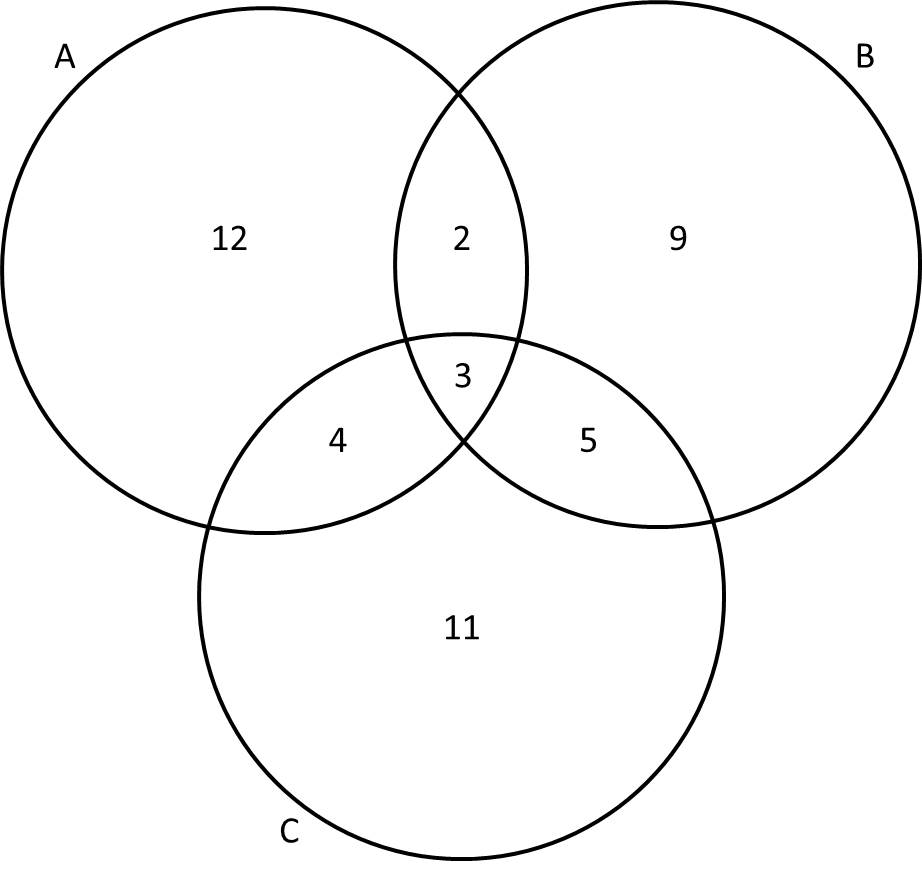
\includegraphics[width=0.25\textwidth]{Venn}
				\caption{Venn diagram}
			\end{figure}
		\end{enumerate}
	\end{description}
	\section{Inclusione, uguaglianza, intersezione e unione di un insieme}
	\begin{definition}{\nmu Inclusione}{inclusione}	
		Siano \textit{A} e \textit{B} due insiemi. Si dice che \textit{A} è incluso in \textit{B} se ogni elemento di \textit{A} è elemento di \textit{B}. L'inclusione si indica con il simbolo:
		\begin{center}
			$A \subseteq B$
		\end{center}
		Se invece non è incluso si indica con:
		\begin{center}
			$A \not \subseteq B$
		\end{center}	
	\end{definition}
	\begin{description}
		\item Alcuni esempi sono:
		\begin{itemize}
			\item \textit{A}: $\{n \in \mathbbm{Z} \mid -1 \leq 5\}$;
			\item \textit{B}: $\{a \in \mathbbm{N} \mid a < 5\}$;
			\item $A \not \subseteq B$ perché $5 \notin B$;
			\item $B \subseteq A$.
		\end{itemize}
	\end{description}
	\begin{note}{}{}
		\begin{center}
		$\mathbbm{N} \subseteq \mathbbm{Z} \subseteq \mathbbm{Q} \subseteq \mathbbm{R}$
	\end{center}
	Si osservi che per ogni insieme \textit{A}, l'insieme vuoto ed \textit{A} stesso risultano essere sottoinsiemi di \textit{A}:
	\begin{center}
		$\emptyset \subseteq A$
		\\$A \subseteq A$
	\end{center}
	
	\end{note}
	\begin{note}{}{}
	Il simbolo appartiene è per gli elementi, il simbolo dell'inclusione è per gli insiemi.	
	\end{note}
	
	\begin{definition}{\nmu Inclusione propria}{inclusione_propria}	
		Sia $A \subseteq B$. Si esiste un elemento di \textit{B} che non è in \textit{A} allora si dice che \textit{A} è incluso propriamente o è sottoinsieme proprio di \textit{B}.
		L'inclusione propria si indica con:
		\[
			A \subsetneq B
		\]
	\end{definition}
	\begin{note}{}{}
	\begin{center}
	$\mathbbm{N} \subsetneq \mathbbm{Z} \subsetneq \mathbbm{Q} \subsetneq \mathbbm{R}$
\end{center}

	\end{note}
	\begin{definition}{\nmu Insiemi uguali}{insiemi_uguali}	
		Sia \textit{A} e \textit{B} insiemi. \textit{A} e \textit{B} sono insiemi uguali se contengono gli stessi elementi, ovvero se:
		\[
		A \subseteq B 
		\]
		\[
		B \subseteq A
		\]
		\[
		A = B		
		\]
		Se non sono uguali:
		\[
			A \neq B
		\]
	\end{definition}
	\noindent
	\\
	\textbf{Ad esempio: }
	\begin{itemize}
		\item \textit{A} = \{$n \in \mathbbm{Z} \mid n \leq 0$\};
		\item \textit{B} = \{$-x \mid x \in \mathbbm{N}$\}
		\item $A = B$.
	\end{itemize}
	\textbf{Notazione: }
	\begin{itemize}
		\item \textbf{Quantificatore universale}: $\forall$, cioè "per ogni";
		\item \textbf{Quantificatore esistenziale}: $\exists$ oppure $\exists!$, cioè "Esiste ed è unico";
		\item $\iff$: Se e solo se.
	\end{itemize}
	\textbf{Proprietà: }
	\begin{itemize}
		\item $\forall$ a,b $\in \mathbbm{N}$ allora a + b $\in \mathbbm{N}$;
		\item $\forall$ a,b $\in \mathbbm{N}$ allora a + b = b + a;
		\item $\forall$ a,b,c $\in \mathbbm{N}$ allora (a + b) + c = a + (b + c);
		\item \textbf{Elemento neutro}: $\exists!$ 0 $\in \mathbbm{N} \mid \forall a \in \mathbbm{N}$ allora a + 0 = 0 + a = a.
	\end{itemize}
	Le prime tre proprietà sono le stesse per la moltiplicazione, la proprietà dell'elemento neutro è sempre uguale ma vale per il numero 1.
	\begin{definition}{\nmu Intersezione}{intersezione}	
		Sia \textit{A} e \textit{B} insiemi. L'insieme intersezione è costituito da tutti gli elementi che appartengono sia ad \textit{A} che a \textit{B} 
		L'intersezione si indica con si indica con:
		\[
		A \cap B = {x \mid x \in A \hspace{0.2cm} e \hspace{0.2cm}x \in B} 
		\]
	\end{definition}
	\noindent
	\textbf{Esempio: }
	\begin{itemize}
		\item \textit{P}: Insieme dei numeri pari = $\{2n \mid n \in \mathbbm{Z}\}$ (0 è PARI);
		\item \textit{D}: Insieme dei numeri dispari = $\{2n + 1 \mid n \in \mathbbm{Z}\}$;
		\item $P \cap D = \emptyset$
	\end{itemize}
	\begin{definition}{\nmu Insiemi disgiunti}{insiemi_disgiunti}	
		Due insiemi \textit{A} e \textit{B} si dicono disgiunti se $A \cap B = \emptyset$
	\end{definition}
	\begin{definition}{\nmu Unione}{unione}	
		Siano \textit{A} e \textit{B} due insiemi. L'insieme unione di \textit{A} e \textit{B} è l'insieme costituito da tutti gli che sono in \textit{A} (inclusivo) o in \textit{B}.
		L'unione di due insiemi si indica con:
		\[
			A \cup B = \{x \mid x \in A \hspace{0.2cm} o \hspace{0.2cm} x \in B\}
		\]
	\end{definition}
	\noindent
	Presi gli insiemi \textit{P} e \textit{D} dell'esempio precedente, segue \textbf{l'esempio}:
	\[P \cup D = \mathbbm{Z}\]
	oppure
	\[\mathbbm{N} \cup \mathbbm{Z} = \mathbbm{Z}\]
	Siano \textit{A}, \textit{B}, \textit{C} insiemi. \textbf{Proprietà.}
	\begin{enumerate}
		\item $A \cup \emptyset = A$;
		\item $A \cap \emptyset = \emptyset$;
		\item $A \cap A = A$;
		\item $A \cup A = A$;
		\item $A \cap B \subseteq  A$ e $A \cap B \subseteq B$;
		\item $A \subseteq A \cup  B$ e $B \subseteq A \cup B$;
		\item Se $A \subseteq B$:
			\begin{enumerate}
				\item $A \cup B = B$;
				\item $A \cap B = A$;
			\end{enumerate}
		\item $A \cup B = B \cup A$;
		\item $A \cap B = B \cap A$;
		\item $(A \cap B) \cap C = A \cap (B \cap C)$;
		\item $(A \cup B) \cup C = A \cup (B \cup C)$;
		\item $(A \cup B) \cap C = (A \cap C) \cup (B \cap C)$
		\item $(A \cap B) \cup C = (A \cup C) \cap (B \cup C)$
	\end{enumerate}
	\section{Complementare, leggi di Demorgan, differenza, insiemi delle parti e prodotto cartesiano}
	\begin{definition}{\nmu Complementare}{complementare}	
		Siano \textit{A} e \textit{B} due insiemi e $B \subseteq A$. Il complementare di \textit{B} in \textit{A} è l'insieme costituito da tutti gli che sono in \textit{A} ma non sono in \textit{B}.
		Il complementare di due insiemi si indica con:
		\[
		C_{A}(B) = \{x \mid x \in A \hspace{0.2cm} e \hspace{0.2cm} x \notin B\}
		\]
	\end{definition}
	\textbf{Esempio: }
	\[
	C_{\mathbbm{Z}}(\mathbbm{N}) = \{x \in \mathbbm{Z} \mid x \notin \mathbbm{N}\} = \{x \in \mathbbm{Z} \mid x < 0\}
	\]
	Siano \textit{A}, \textit{B} e \textit{C} insiemi e $B \subseteq A$ e $C \subseteq A$. \textbf{Proprietà: }
	\begin{enumerate}
		\item $C_{A}(B) \cup B = A$;
		\item $C_{A}(B) \cap B = \emptyset$;
		\item $C_{A}(A) = \emptyset$;
		\item $C_{A}(\emptyset) = A$
		\item $C_{A}(B \cup C) = C_{A}(B) \cap C_{A}(C)$;
		\item $C_{A}(B \cap C) = C_{A}(B) \cup C_{A}(C)$.
	\end{enumerate}
	\textbf{Nota: } Le proprietà 5, 6 prendono il nome di \textbf{leggi di Demorgan.}
	\begin{proof}{Dimostrazione della prima legge di Demorgan: \[C_A(B \cup C) = C_A(B) \cap C_A(C)\]}	\quad \\
		Per dimostrare la prima legge di Demorgan dobbiamo dimostrare due cose:
		\begin{enumerate}
			\item $C_{A}(B \cup C) \subseteq C_{A}(B) \cap C_{A}(C)$
				\begin{enumerate}
					\item Dobbiamo dimostrare che $\forall x \in C_{A}(B \cup C)$ si ha che $x \in C_{A}(B) \cap C_{A}(C)$:
					\item Sia $x \in C_{A}(B \cup C)$ allora $x \in A$ e $x \notin B \cup C$ allora $x \notin B$ e $x \notin C$, quindi: $x \in C_{A}(B)$ e $x \in C_{A}(C)$ allora $x \in C_{A}(B) \cap C_{A}(C)$
					\item $\forall x \in C_{A}(B) \cap C_{A}(C)$ si ha che $x \in C_{A}(B \cup C)$
					\item Sia $x \in C_{A}(B) \cap C_{A}(C)$ allora $x \in C_{A}(B)$ e $x \in C_{A}(C)$ allora $x \in A$ e $x \notin B$ e $x \notin C$ allora $x \in A$ e $x \notin B \cup C$ allora $x \in C_{A}(B \cup C)$
				\end{enumerate}
			\item $C_{A}(B) \cap C_{A}(C) \subseteq C_{A}(B \cup C)$
				\begin{enumerate}
					\item Dobbiamo dimostrare che $\forall x \in C_{A}(B) \cap C_{A}(C)$ si ha che $x \in C_{A}(B \cup C)$
					\item Sia $x \in C_{A}(B) \cap C_{A}(C)$ allora $x \in A, x \notin B, x \notin C$ allora $x \in A, x \notin B \cup C$ pertanto $x \in C_{A}(B \cup C)$
					\item $\forall x \in C_{A}(B \cup C)$ si ha che $x \in C_{A}(B) \cap C_{A}(C)$.
					\item Sia $x \in C_{A}(B \cup C)$ allora $x \in A, x \notin B, x \notin C$ allora $x \in C_{A}(B) \cap C_{A}(C)$
				\end{enumerate}
		\end{enumerate}
	\end{proof}
	\begin{proof}{Dimostrazione della seconda legge di Demorgan: \[
			C_A(B \cap C) = C_A(B) \cup C_A(C)
			\]}	 \quad \\
		Per dimostrare la seconda legge di Demorgan dobbiamo dimostrare due cose:
		\begin{enumerate}
			\item $C_{A}(B \cap C) \subseteq C_{A}(B) \cup C_{A}(C)$
				\begin{enumerate}
					\item Dobbiamo dimostrare che $\forall x \in C_{A}(B \cap C)$ si ha che $x \in C_{A}(B) \cup C_{A}(C)$
					\item Sia $x \in C_{A}(B \cap C)$ dato che $B \subseteq A$ e $C \subseteq A$, $x \in A$, $x \notin B \ o \ x \notin C$, allora $x \in C_{A}(B) \cup C_{A}(C)$ 
				\end{enumerate}
			\item $C_{A}(B) \cup C_{A}(C) \subseteq C_{A}(B \cap C)$
				\begin{enumerate}
					\item Dobbiamo dimostrare che $\forall x \in C_{A}(B) \cup C_{A}(C)$ si ha che $x \in C_{A}(B \cap C)$
					\item Sia $x \in C_{A}(B) \cup C_{A}(C)$ o $x \in C_{A}(B) \ o \ x \in C_{A}(C)$, allora $x \in A, x \notin B \ o \ x \notin C$ e $x \in C_{A}(B \cap C)$
					
				\end{enumerate}
		\end{enumerate}
	
	\end{proof}
	\begin{definition}{\nmu Insieme differenza}{insieme_differenza}	
		Siano \textit{A} e \textit{B} due insiemi. L'insieme differenza tra \textit{A} e \textit{B} è l'insieme di tutti gli elementi che sono in \textit{A} e non sono in \textit{B}.
		L'insieme differenza si indica con:
		\[
			A \backslash B \hspace{0.2cm} oppure \hspace{0.2cm} A - B
		\]
		Questa è una generalizzazione di complementare perché non è richiesto che $B \subseteq A$.
	\end{definition}
	\newpage
	\textbf{Osservazione: }
	\[
		Se B \subseteq A \ allora \ C_{A}(B) = A \backslash B
	\]
	\[
		A \backslash B = C_{A}(A \cap B)
	\]
	\begin{definition}{\nmu Prodotto cartesiano}{prod_cartesiano}	
		Siano \textit{A} e \textit{B} due insiemi. Il prodotto cartesiano di \textit{A} per \textit{B} è l'insieme degli elementi costituito da tutte le coppie ordinate $(a, b)$ con $a$ appartenente ad \textit{A} e $b$ appartenente a \textit{B}.
		Il prodotto cartesiano si indica con:
		\[
		A \times B = \{(a, b) \mid a \in A \ e \ b \in B\}
		\]
	\end{definition}
	\textbf{Esempio: }
	\[
		\mathbbm{R} \times \mathbbm{R} = \{(x, y) \mid x \in \mathbbm{R} \ e \ y \in \mathbbm{R}\}
	\]
	Questo rappresenta le coordinate del diagramma cartesiano.
	\begin{definition}{\nmu Insieme delle parti}{insieme_parti}	
		Siano \textit{A} un insieme. L'insieme delle parti di \textit{A} è l'insieme dei sottoinsiemi di \textit{A}. Gli elementi dell'insieme delle parti di $A$ sono tutti e soli sottoinsiemi di $A$.
		L'insieme delle parti si indica con:
		\[
		\wp(A) = \{x \ insieme \ \mid x \subseteq A\}
		\]
	\end{definition}
	\textbf{Osservazioni: }
	\begin{itemize}
		\item Se $a \in A$ allora $\{a\} \subseteq A \ allora \ \{a\} \in \wp(A)$
		\item $\emptyset \in \wp(A)$
		\item $A \subseteq A \ allora \ A \in \wp(A)$
	\end{itemize}
	\textbf{Esempio:}
	$A = \{a, b, c, d\}$
	\\ $\wp(A)$ = \{$\emptyset$, A = \{a, b, c, d\}, \{a\}, \{b\}, \{c\}, \{d\}, \{a, b\}, \{a, c\}, \{a, d\}, \{b, c\},\{b, d\}, \{d, c\}, \{a, b, c\}, \{a, b, d\}, \{a, c, d\}, \{a, c, d\}, \{b, c, d\}\}
	
	\chapter{Logica}
	\section{Proposizioni, definizione di negazione, congiunzione e disgiunzione, implicazione}
	Una proposizione logica è un'affermazione di cui si può stabilire se è vera o falsa, solo una delle due.
	\\
	\textbf{Esempi: }
	\begin{itemize}
		\item Il cane è un mammifero. Questa proposizione è vera, quindi 1 o V o T.
		\item X è un numero positivo. Questa non è una proposizione perché non si può stabilire se vera o falsa.
	\end{itemize}
	\begin{definition}{\nmu Negazione}{negazione}	
		Sia $P$ una proposizione. La negazione di $P$ è una proposizione che è vera se $P$ è falsa e falsa se $P$ è vera.
		I simboli della negazione sono:
		
		\[
		\overline P \ oppure \ ^\neg P
		\]
	\end{definition}
	\textbf{Esempio: }
	\begin{enumerate}
		\item \textit{P: }Roma è una città del Lazio. V
		\begin{itemize}
			\item $\overline P:$ Non è vero che Roma è una città del Lazio.
		\end{itemize}
		\item $P: \forall y \in \mathbbm{N} \ y $ è $> 3$. Falsa perché non è vero che ogni $y > 3$ infatti $\exists 0 \in \mathbbm{N}$ che non è $> 3$.
		\begin{itemize}
			\item $\overline P:$ Non è vero che $\forall y \in \mathbbm{N}$ $> 3$ oppure $\exists y \in \mathbbm{N} \mid \ y$ non è $> 3$.
			\item La negazione di P del secondo esempio non è $\forall y \notin \mathbbm{N} $ non è $> 3$ perché $\exists 4 \in \mathbbm{N}$.
		\end{itemize}
		\item $R: \forall x \in \mathbbm{N} \ \exists y \in \mathbbm{N} \mid x + y - 3 = 0$.
		\begin{itemize}
			\item $\overline R:$ Non è vero che $\forall x \in \mathbbm{N} \ \exists y \mid x + y - 3 = 0$ perché $\exists x \in \mathbbm{N} \mid \forall y \in \mathbbm{N} \ x + y - 3 \not = 0$
		\end{itemize}
		\item $S: \exists x \in \mathbbm{N} \ e \ \exists y \in \mathbbm{Z} \mid x + y + 4 \not = 0$. $S$ è vera.
		\begin{itemize}
			\item $\overline S: \forall x \in \mathbbm{N} \ e \ \forall y \in \mathbbm{Z} \mid x + y + 4 = 0$
		\end{itemize}
	\end{enumerate}
	\textbf{Tavola di verità}	
	\\
	\\
	\begin{tabular} {c|c}
		$\mathbf{P}$ & $\mathbf{\overline P}$ \\
		\hline
		V & F \\
		F & V \\
	\end{tabular}

	\begin{definition}{\nmu Congiunzione}{congiunzione}	
		Sia $P$ e $Q$ due proposizioni. La proposizione congiunzione di $P$ e $Q$, si legge "P e Q" è una proposizione che è vera solo quando entrambe sono vere ed è falsa solo quando entrambe sono false.
		I simboli della congiunzione sono:
		\[
		P \wedge Q
		\]
	\end{definition}
	\textbf{Tavola di verità}
	\\
	\\
	\begin{tabular}{c|c|c}
		$\mathbf{P}$ & $\mathbf{Q}$ & $\mathbf{P \wedge Q}$ \\
		\hline
		V & V & V\\
		V & F & F\\
		F & V & F\\
		F & F & F\\
	\end{tabular}
	\\
	\\	
	\textbf{Esempio: }
	\begin{enumerate}
		\item $P:$ 6 è un numero pari. V
		\item $Q:$ 6 è multiplo di 4. F
		\begin{itemize}
			\item $P \wedge Q: $ 6 è un numero pari ed è multiplo di 4 è falsa.
		\end{itemize}
	\end{enumerate}
	\begin{definition}{\nmu Disgiunzione}{disgiunzione}	
		Sia $P$ e $Q$ due proposizioni. La proposizione disgiunzione di $P$ e $Q$, che si legge "P o Q", è una proposizione che è falsa solo quando entrambe sono false, altrimenti è vera.
		I simboli della disgiunzione sono:
		\[
		P \vee Q
		\]
	\end{definition}
	\textbf{Tavola di verità:}
	\\
	\\
	\begin{tabular}{c|c|c}
		$\mathbf{P}$ & $\mathbf{Q}$ & $\mathbf{P \vee Q}$ \\
		\hline
		V & V & V \\
		V & F & V \\
		F & V & V \\
		F & F & F \\
	\end{tabular}
	\\
	\\
	\textbf{Esempi: }
	\begin{enumerate}
		\item $P \vee Q$: 6 è un numero pari o 6 è un multiplo di 4. Questa proposizione è vera.
	\end{enumerate}
	\textbf{Esercizio: } Scrivere tavole di verità di $P \wedge \overline P$ e $P \vee \overline P$.
	\\
	\\
	\begin{tabular}{c|c|c}
		$\mathbf{P}$ & $\mathbf{\overline P}$ & $\mathbf{P \wedge \overline P}$ \\
		\hline
		V & F & F\\ 
		F & V & F\\ 
 	\end{tabular}
	\\
	\textbf{Nota: }
	\\
	Proposizione sempre falsa si dice CONTRADDIZIONE.
	\\
	\\
	\begin{tabular}{c|c|c}
	$\mathbf{P}$ & $\mathbf{\overline P}$ & $\mathbf{P \vee \overline P}$ \\
	\hline
	V & F & V\\ 
	F & V & V\\ 
	\end{tabular}
	\\
	\textbf{Nota: }
	\\
	Proposizione sempre vera si chiama TAUTOLOGIA.
	\begin{definition}{\nmu Implicazione}{implicazione}	
		Sia $P$ e $Q$ due proposizioni. La proposizione implicazione di $P$ e $Q$, che si legge "se P allora Q", è una proposizione che è falsa solo se P è vera e Q è falsa ed è vera altrimenti.
		I simboli dell'implicazione sono:
		\[
		P \to Q
		\]
	\end{definition}
	\textbf{Tavola di verità:}
	\\
	\\
	\begin{tabular}{c|c|c}
		$\mathbf{P}$ & $\mathbf{Q}$ & $\mathbf{P \to Q}$ \\
		\hline
		V & V & V \\
		V & F & F \\
		F & V & V \\
		F & F & V \\
	\end{tabular}
	\\
	\\
	\textbf{Esempi:}
	\begin{enumerate}
		\item P: Io vado sulla luna.
		\item Q: Ti regalo una stella.
		\begin{itemize}
			\item $P \to Q$: Se io vado sulla luna allora ti regalo una stella
		\end{itemize}
	\end{enumerate}
	\textbf{Differenza: }
	\\
	IF...THEN di programmazione perchè se in programmazione la condizione dell'if fallisce il programma non esegue più il costrutto mentre in matematica la proposizione rimane comunque vera.
	\newpage
	\begin{definition}{\nmu Doppia implicazione}{doppia_implicazione}	
		Sia $P$ e $Q$ due proposizioni. La doppia implicazione di $P$ e $Q$, che si legge "P se e solo se Q", è una proposizione che è vera quando P e Q sono entrambe vere o entrambe false.
		I simboli dell'implicazione sono:
		\[
		P \leftrightarrow  Q
		\]
	\end{definition}
	\textbf{Tavola di verità:}
	\\
	\\
	\begin{tabular}{c|c|c}
		$\mathbf{P}$ & $\mathbf{Q}$ & $\mathbf{P \leftrightarrow Q}$ \\
		\hline
		V & V & V \\
		V & F & F \\
		F & V & F \\
		F & F & V \\
	\end{tabular}
	\\
	\\
	Quindi la doppia implicazione è vera quando sono vere entrambe le implicazioni $P \to Q$ e $Q \to P$.
	\\
	\textbf{Tavola di verità:}
	\\
	\\
	\begin{tabular}{c|c|c|c|c}
		$\mathbf{P}$ & $\mathbf{Q}$ & $\mathbf{P \to Q}$ & $\mathbf{Q \to P}$ & $\mathbf{P \leftrightarrow Q}$ \\
		\hline
		V & V & V & V & V \\
		V & F & F & V & F \\
		F & V & V & F & F \\
		F & F & V & V & V \\
	\end{tabular}
	\\
	\\
	\textbf{Osservazione: }
	\\
	$P \leftrightarrow Q$ è una proposizione.
	\\
	$P \iff Q$ è un simbolo che ci dice che $P \leftrightarrow Q$ è una proposizione sempre vera, questo si verifica solo e solo se P e Q sono entrambe vere o false.
	\\
	Analogamente il simbolo $P \Rightarrow Q$ indica che la proposizione $P \to Q$ è vera, quindi l'unico caso da escludere è il caso in cui P è vera e Q è falsa.
	Quindi si deve dimostrare che se P è vera anche Q è necessariamente vera.
	\newpage
	\textbf{Esercizio:} Dimostrare che sono equivalenti le seguenti proposizioni.
	\begin{itemize}
		\item $\overline {P \wedge Q} \iff \overline P \vee \overline Q$
	\end{itemize}

	\begin{tabular}{c|c|c|c|c|c|c}
		$\mathbf{P}$ & $\mathbf{Q}$ & $\mathbf{\overline P}$ & $\mathbf{\overline Q}$ & $\mathbf{\overline P \vee \overline Q}$ & $\mathbf{P \wedge Q}$ & $\mathbf{\overline{P \wedge Q}}$ \\
		\hline
		V & V & F & F & F & V & F\\
		V & F & F & V & V & F & V\\
		F & V & V & F & V & F & V\\
		F & F & V & V & V & F & V\\
	\end{tabular}
	\\
	\textbf{Esercizio per casa: }
	Dimostrare: $\overline{P \vee Q} \iff \overline P \wedge \overline Q$
	\\
	\\
	\begin{tabular}{c|c|c|c|c|c|c}
		$\mathbf{P}$ & $\mathbf{Q}$ & $\mathbf{\overline P}$ & $\mathbf{\overline Q}$ & $\mathbf{\overline P \wedge \overline Q}$ & $\mathbf{P \vee Q}$ & $\mathbf{\overline{P \vee Q}}$ \\
		\hline
		V & V & F & F & F & V & F \\
		V & F & F & V & F & V & F \\
		F & V & V & F & F & V & F \\
		F & F & V & V & V & F & V \\
	\end{tabular}
	\\
	\textbf{Esercizio: }
	\\
	Dimostrare $P \to Q \centernot \iff P \to \overline Q$ e $P \to Q \iff \overline Q \to \overline P$
	\\
	\\
	\begin{tabular}{c|c|c|c|c|c|c|c}
		$\mathbf{P}$ & $\mathbf{Q}$ & $\mathbf{\overline P}$ & $\mathbf{\overline Q}$ & $\mathbf{P \to Q}$ & $\mathbf{Q \to P}$ & $\mathbf{P \to \overline Q}$ & $\mathbf{\overline Q \to \overline P}$ \\
		\hline
		V & V & F & F & V & V & F & V\\
		V & F & F & V & F & V & V & F\\
		F & V & V & F & V & F & V & V\\
		F & F & V & V & V & V & V & V\\
	\end{tabular}
	\\
	\textbf{Per casa: } Studiare $Q \to P$ e se è equivalente ad una delle 3 colonne della tabella precedente.
	\\
	No, non è equivalente a nessuna delle ultime 3 colonne della tabella precedente.
	\\
	\textbf{Esercizio: }Dimostrare $(P \wedge Q) \wedge R \iff (P \vee R) \wedge (Q \vee R)$
	\\
	\\
	\begin{tabular}{c|c|c|c|c|c|c|c}
		$\mathbf{P}$ & $\mathbf{Q}$ & $\mathbf{R}$ & $\mathbf{P \wedge Q}$ & $\mathbf{(P \wedge Q) \wedge R}$ & $\mathbf{P \vee R}$ & $\mathbf{Q \vee R}$ & $\mathbf{(P \vee R) \wedge (Q \vee R)}$ \\
		\hline
		V & V & V & V & V & V & V & V\\
		V & V & F & F & F & V & V & V\\
		V & F & V & F & F & V & V & V\\
		V & F & F & F & F & V & V & V\\
		F & V & V & F & F & V & V & V\\
		F & V & F & F & F & V & V & V\\
		F & F & V & F & F & V & V & V\\
		F & F & F & F & F & F & F & F\\ 
	\end{tabular}
	\\
	\\
	$(P \wedge Q) \wedge R \centernot \iff (P \vee R) \wedge (Q \vee R)$.
	\\
	\textbf{Esercizio: }Dimostrare $(P \wedge Q) \vee R \iff (P \vee R) \wedge (Q \vee R)$
	\\
	\\
	

	\newpage
	\textbf{Esercizio:} $\exists s \in \mathbbm{N} \mid \forall b \in \mathbbm{Z} \ \exists q \in \mathbbm{R}$ con $b + s - q = 0$.
	\begin{itemize}
		\item $q = b + s \in \mathbbm{R}$
		\item $\exists s = 0 \in \mathbbm{N} \mid \ \forall b \in \mathbbm{Z} \ \exists q = b \in \mathbbm{R}$
		\item $b + s - q = b + 0 - b = 0$. P è vera		
	\end{itemize}

	$\overline P: \forall s \in \mathbbm{N} \ \exists b \in \mathbbm{Z} \mid \forall q \in \mathbb{R} \ b + s - q \not = 0$.
	\\
	\\
	\textbf{Esercizio:} $Q: \exists s \in \mathbbm{N} \mid \forall b \in \mathbbm{R} \ \exists q \in \mathbbm{Z}$ con $b + s - q = 0$.
	\begin{itemize}
		\item $q = b + s \in \mathbbm{Z} \ ? $. Q  non è vera
	\end{itemize}

	$\overline Q: \forall s \in \mathbbm{N} \ \exists b \in \mathbbm{R} \mid \forall q \in \mathbbm{Z}$ con $b + s - q \not = 0$
	\begin{itemize}
		\item $\forall s \in \mathbbm{N} \ \exists \sqrt{2} \in \mathbbm{R} \mid \forall q \in \mathbbm{Z}$ con $\sqrt{2} + s - q \not = 0$
	\end{itemize}
	\textbf{Esercizio:} $S: \forall x \in \mathbbm{Z} \ \exists t \in \mathbbm{N} \ e \ \exists y \in \mathbbm{N} \mid x = t^2 + y$
	\\
	S è falsa perché $x \in \mathbbm{Z}$ e può essere negativo mentre $t \in \mathbbm{N} \ e \ y \in \mathbbm{N}$ pertanto $t^2 + y \geq 0$.
	\\ 
	$\overline S: \exists x \in \mathbbm{Z} \mid \forall t \in \mathbbm{N} \ e \ \forall y \in \mathbbm{N} \ x \not = t^2 + y$
	\\
	\textbf{Esercizio:} $S: \forall x \in \mathbbm{Z} \ \exists t \in \mathbbm{N} \ e \ \exists y \in \mathbbm{N} \mid x^2 = t^2 + y$
	\\
	$\forall x \in \mathbbm{Z} \ \exists t = 0 \in \mathbbm{N}$ e $\exists y = x^2$
	\\ 
	$\overline S: \exists x \in \mathbbm{Z} \mid \forall t \in \mathbbm{N} \ e \ \forall y \in \mathbbm{N} x \not = t^2 + y$
	\chapter{Funzioni}
	\section{Definizione di funzione, funzioni che coincidono, immagine, controimmagine, grafico}
	\begin{definition}{\nmu Funzione}{funzione}	
		Siano $A$ e $B$ due insiemi non vuoti. Una funzione dall'insieme $A$ all'insieme $B$ è una legge che associa ad ogni elemento di $A$ un unico elemento dell'insieme $B$.
		\\
		Simbolo della funzione:
		\[
		f: A \to B
		\]
		$A$ è l'insieme di partenza detto anche \textit{dominio} di f.
		\\
		$B$ è l'insieme di arrivo di $f$.
	\end{definition}
	$f: A \to B$
	\\
	$a \longmapsto f(a) \in B$
	\\
	$\mathit{f}(a) = b$ ed equivale all'immagine di $A$.
	\\
	$\forall a \in A \ \exists! \ b \in B \mid f(a) = b$
	\\
	\textbf{Esempi:}
	\begin{enumerate}
		\item $f: \mathbbm{N} \to \mathbbm{N}$
			\begin{itemize}
				\item 	$\forall a \in \mathbbm{N} \ f(a) = a - 4$ \\ Non è una funzione perché $\exists a \in \mathbbm{N} \mid a - 4 \notin \mathbbm{N}$
			\end{itemize}
		\item $g: \mathbbm{N} \to \mathbbm{Z}$
			\begin{itemize}
				\item $\forall a \in \mathbbm{N} \ g(a) = a - 4 \in \mathbbm{Z}$ \\ Questa è una funzione.
			\end{itemize}
		\item $h: \mathbbm{Q} \to \mathbbm{R}$
			\begin{itemize}
				\item $\forall x \in \mathbbm{Q} h(x) = \frac{4}{x - 3}$
				\\
				Non è una funzione perché $h(3)$ non è definito.
			\end{itemize}
		\item $f: \mathbbm{Q} \backslash \{3\} \to \mathbbm{R}$
			\begin{itemize}
				\item  $\forall x \in \mathbbm{Q} \backslash \{3\} f(x) = \frac{4}{x - 3}$
				\\
				Questa è una funzione.
			\end{itemize}
	\end{enumerate}

	\begin{definition}{\nmu Funzioni uguali}{funzioni_uguali}	
		Due funzioni si dicono uguali se hanno stesso insieme di partenza, stesso insieme di arrivo e stessa legge.
	\end{definition}
	\textbf{Esempio: }
	\\
	$f: \mathbbm{R} \to \mathbbm{R} \ \forall x \in \mathbbm{R} \ f(x) = 6x + 4$
	\\
	$g: \mathbbm{R} \to \mathbbm{R} \ \forall t \in \mathbbm{R} \ g(t) = 2(3t + 2)$
	\\
	\textbf{Esempio di funzione COSTANTE: }
	\\
	$A \neq \emptyset \ B \neq \emptyset \ e fissiamo \ b_{0} \in B$
	\\
	Allora è definita la funzione costante $b_{0}$ che ad ogni elemento di A associa $b_{0}$.
	\\
	$f: A \to B \ \forall a \in A \ f(a) = b_{0}$.
	\\
	\textbf{Esempio: }
	\\
	$f: \mathbbm{R} \to \mathbbm{R} \ \forall x \in \mathbbm{R} \ f(x) = 4$.
	\\
	$f(-\pi) = 4$.
	\\
	$f(3^5) = 4$.
	\\
	\textbf{Esempio di funzione IDENTICA o IDENTITÀ: }
	\\
	$\forall A \ insieme \ non \ vuoto \ \exists \ la \ funzione \ I_{d_{A}}: A \to A \ \forall a \in A \ I_{d_{A}}(a) = a$, cioè ogni elemento viene mandato in se stesso.
	
	\begin{definition}{\nmu Immagine}{immagine}	
		L'immagine di una funzione $f: A \to B$ si indica con $Im(f)$ o $f(A)$ ed è il sottoinsieme di $B$ costituito da tutte le immagini degli elementi di $A$, ovvero:
		\\
		$f(A) \subseteq B \ f(A) = \{b \in B \mid \exists a \in A \ con \ f(a) = b \}$
		\\
		In generale, dato un sottoinsieme $A' \subseteq A$. Si definisce l'immagine di $A'$ il sottoinsieme $f(A') \subseteq B$ con
		\[
		f(A') = \{b \in B \mid \exists a \in A' \ con \ f(a) = b\} = \{f(a) \mid a \in A'\}
		\]
	\end{definition}
	
	\textbf{Esempio: }
	\\
	$g: \mathbbm{Z} \to \mathbbm{Z} \ \forall s \in \mathbbm{Z} \ g(s) = 4s$
	\\
	Determina $g(\mathbbm{Z})$ e $g(A') \ con \ A' = \{1, -1, -3, 4, 0\}$
	\\
	$g(\mathbbm{Z}) = \{b \in \mathbbm{Z} \mid \exists a \in \mathbbm{Z} \ g(a) = b\} = \{b \in \mathbbm{Z} \mid \exists a \in \mathbbm{Z} \ con \ 4a = b\}$
	\\
	$g(A') = \{b \in \mathbbm{Z} \mid \exists a \in A' \ con \ g(a) = b\} = \{b \in \mathbbm{Z} \mid \exists a \in A' \ con \ 4a = b\}$	
	$g(A') = \{4, -4, -12, 16, 0\}$.
	\\
	\textbf{Esempio: }
	\\
	$f: \mathbbm{N} \to \mathbbm{N} \ \forall n \in \mathbbm{N} \ con \ f(n) = n + 3$
	\\
	$f(\mathbbm{N}) = \mathbbm{N} \backslash \{0, 1, 2\}$
	
	\begin{definition}{\nmu Controimmagine}{controimmagine}	
		Siano $f: A \to B$ una funzione e $Y \subseteq B$. La controimmagine di $Y$ oppure immagine inversa di $Y$, è il sottoinsieme di $A$ costituito da tutti gli elementi la cui immagine è in $Y$.
		\\
		Simbolo della controimmagine:
		\[
		f^{-1}(Y)
		\]
		$f^{-1}(Y) \subseteq A = \{a \in A \mid f(a) \in Y\}$
		\\
		In particolare $f^{-1}(B) = \{a \in A \mid f(a) \in B\} = A$
	\end{definition}	
	\textbf{Proprietà: }
	\\
	Siano $f: A \to B$ funzione. $X, X' \subseteq A \ e \ Y, Y' \subseteq B$. 
	\\
	Allora:
	\begin{enumerate}
		\item $f(X \cap X') \subseteq f(X) \cap f(X')$
		\item $f(X \cup X') = f(X) \cup f(X')$
		\item $f^{-1}(Y \cap Y') = f^{-1}(Y) \cap f^{-1}(Y')$
		\item $f^{-1}(Y \cup Y') = f^{-1}(Y) \cup f^{-1}(Y')$
	\end{enumerate}
	\begin{proof}{Dimostrazione di $f(X \cap X') \subseteq f(X) \cap f(X')$} \quad \\
		Sia $b \in f(X \cap X') \subseteq B \\ \Rightarrow b = f(a) \ con \ a \in X \cap X' \\ \Rightarrow b = f(a) \ con \ a \in X \ e \ a \in X' \\ \Rightarrow b \in f(X) \ e \ b \in f(X') \\ \Rightarrow b \in f(X) \cap f(X')$
	\end{proof}
	\textbf{Esempio: }
	\\
	$f(X) \cap f(X') \not \subseteq f(X \cap X')$
	\\
	Sia $f: \mathbbm{R} \to \mathbbm{R} \ \forall a \in \mathbbm{R} \ f(a) = a^2$
	\\
	$X = \{0, 2\} \ X' = \{0, -2\}$
	\\
	$X \cap X' = \{0\}$
	\\
	$f(X \cap X') = f(\{0\}) = f(0) = \{0\}$
	\\
	$f(\{0, 2\}) = \{b \in \mathbbm{R} \mid \exists q \in \{0, 2\} \ g(a) = b\} = \{g(a) \in \mathbbm{R} \mid a \in \{0,2\}\} = \{g(0), g(2)\} = \{0^2, 2^2\} = \{0, 4\}$.
	\\
	$f(\{0, -2\}) = \{0, 4\}$
	\\
	$f(X) \cap f(X') = \{0, 4\} \not \subseteq f(X \cap X') = \{0\}$
	
	\begin{proof}{Dimostrazion di $f(X \cup X') {=} f(X) \cup f(X')$} \quad \\
		Dobbiamo dimostrare due cose:
		\begin{enumerate}
			\item $f(X \cup X') \subseteq f(X) \cup f(X')$
				\begin{itemize}
					\item Se $b \in f(X \cup X') \Rightarrow b \in f(X) \cup f(X')$
					\begin{itemize}
						\item Sia $b \in f(X \cup X') \\ \Rightarrow b = f(a) \ con \ a \in X \cup X' \\ \Rightarrow b = f(a) \ con \ a \in X \ o \ a \in X' \\ \Rightarrow b \in f(X) \ o \ b \in f(X') \\ \Rightarrow b \in f(X) \cup f(X')$
					\end{itemize}

				\end{itemize}
			\item $f(X) \cup f(X') \subseteq f(X \cup X')$
				\begin{itemize}
					\item Se $b \in f(X) \cup f(X') \Rightarrow b \in f(X \cup X')$
					\begin{itemize}
						\item Sia $b \in f(X) \cup f(X') \\ \Rightarrow b = f(a) \ con \ a \in X \ o \ a \in X' \\ \Rightarrow b = f(a) \ con \ a \in X \cup X' \\ \Rightarrow b \in f(X \cup X')$
					\end{itemize}
				\end{itemize} 
		\end{enumerate}
	\end{proof}
	
	\begin{proof}{Dimostrazione di $f^{-1}(Y \cap Y') {=} f^{-1}(Y) \cap f^{-1}(Y')$}
		Dobbiamo dimostrare due cose:
		\begin{enumerate}
			\item $f^{-1}(Y \cap Y') \subseteq f^{-1}(Y) \cap f^{-1}(Y')$
				\begin{itemize}
					\item Se $a \in f^{-1}(Y \cap Y') \Rightarrow a \in f^{-1}(Y) \cap f^{-1}(Y')$
					\begin{itemize}
						\item Sia $a \in f^{-1}(Y \cap Y') \mid f(a) = b \in Y \cap Y' \\ \Rightarrow a \in f^{-1}(Y \cap Y') \mid f(a) = b \in Y \ e \ b \in Y' \\ \Rightarrow a \in f^{-1}(Y) \cap f^{-1}(Y')$
					\end{itemize}
				\end{itemize}
			\item $f^{-1}(Y) \cap f^{-1}(Y') \subseteq f^{-1}(Y \cap Y')$
				\begin{itemize}
					\item Se $a \in f^{-1}(Y) \cap f^{-1}(Y') \Rightarrow a \in f^{-1}(Y \cap Y')$
					\begin{itemize}
						\item Sia $a \in f^{-1}(Y) \cap f^{-1}(Y') \mid f(a) = b \in Y \ e \ b \in Y' \\ \Rightarrow a \in f^{-1}(Y) \cap f^{-1}(Y') \mid b \in Y \cap Y' \\ \Rightarrow a \in f^{-1}(Y \cap Y')$
					\end{itemize}
				\end{itemize}
		\end{enumerate}
	\end{proof}
	
	\begin{proof}{Dimostrazione di $f^{-1}(Y \cup Y') {=} f^{-1}(Y) \cup f^{-1}(Y')$ } \quad \\
		Dobbiamo dimostrare due cose:
		\begin{enumerate}
			\item $f^{-1}(Y \cup Y') \subseteq f^{-1}(Y) \cup f^{-1}(Y')$
			\begin{itemize}
				\item Se $a \in f^{-1}(Y \cup Y') \Rightarrow a \in f^{-1}(Y) \cup f^{-1}(Y')$
				\begin{itemize}
					\item Sia $a \in f^{-1}(Y \cup Y') \mid f(a) = b \in Y \cup Y' \\ \Rightarrow a \in f^{-1}(Y \cup Y') \mid f(a) = b \in Y \ o \ b \in Y' \\ \Rightarrow a \in f^{-1}(Y) \cup f^{-1}(Y')$
				\end{itemize}
			\end{itemize}
			\item $f^{-1}(Y) \cup f^{-1}(Y') \subseteq f^{-1}(Y \cup Y')$
			\begin{itemize}
				\item Se $a \in f^{-1}(Y) \cup f^{-1}(Y') \Rightarrow a \in f^{-1}(Y \cup Y')$
				\begin{itemize}
					\item Sia $a \in f^{-1}(Y) \cup f^{-1}(Y') \mid f(a) = b \in Y \ o \ b \in Y' \\ \Rightarrow a \in f^{-1}(Y) \cup f^{-1}(Y') \mid b \in Y \cup Y' \\ \Rightarrow a \in f^{-1}(Y \cup Y')$
				\end{itemize}
			\end{itemize}
		\end{enumerate}
	\end{proof}
	
	\begin{definition}{\nmu Grafico}{grafico}
		Il grafico  di una funzione $f: A \to B$ è il sottoinsieme del prodotto cartesiano $A \times B$ costituito dalle coppie ordinate $(a, f(a))$, al variare di $a \in A$.
	\end{definition}	
	Prendendo l'esempio precedente il grafico è $\{(a, a^2) \in \mathbbm{R} \times \mathbbm{R} \mid a \in \mathbbm{R}\}$
	\section{Funzione iniettiva, suriettiva, biunivoca}
	\begin{definition}{\nmu Funzione iniettiva}{func_iniettiva}	
		Sia $f: A \to B$ una funzione $f$ è detta iniettiva se elementi distinti di A hanno immagini distinte in B.
		
		\[
		\forall a, a' \in A \ se \ a' \neq a \Rightarrow f(a) \neq f(a')
		\]
		Questo equivale a dire che se $f(a) = f(a') \Rightarrow a = a'$  
	\end{definition}
	\textbf{Osservazione: }
	\\
	$f$ non è iniettiva se $\exists a, a' \in A \ con \ a \neq a' \ e \ f(a) = f(a')$.
	\\
	\textbf{Esempi: }
	\\
	$f: \mathbbm{Z} \to \mathbbm{Z} \forall a \in \mathbbm{Z} \ f(a) = 3a + 5$
	\\
	F è iniettiva se $\forall a, a' \in \mathbbm{Z} \ f(a) = f(a') \Rightarrow a = a'$.
	\\
	$f(a) = f(a') \\ \Rightarrow 3a + 5 = 3a' + 5 \\ \Rightarrow 3a = 3a' \\ \Rightarrow a = a'$. Questa funzione è iniettiva.
	\\
	\textbf{Secondo esempio: }
	\\
	$g: \mathbbm{Z} \to \mathbbm{Z} \ \forall x \in \mathbbm{Z} \ g(x) = x^2$
	\\
	$\forall a, a' \in \mathbbm{Z} \ g(a) = g(a') \Rightarrow a = a'$
	\\
	$g(a) = g(a') \\ \Rightarrow a^2 = a'^2 \\ \Rightarrow a = a' \ o \ a = -a'$. In questo caso la funzione non è iniettiva.
	\\
	Secondo modo:
	\\
	$\exists \ 2, -2 \in \mathbbm{Z} \mid 2 \neq -2 \ e \ g(2) = 4 = g(-2)$
	\\
	\textbf{Terzo esempio: }
	\\
	$f: \mathbbm{Z} \to \mathbbm{Z} \ \forall x \in \mathbbm{Z} \ f(x) = \mid x \mid$
	\\
	$\mid x \mid$ = 
	$\begin{cases*}
		-x & se $x < 0$ \\
		\phantom{-}x & se $x \geq 0$
	\end{cases*}$
	\\
	$\forall a, a' \in \mathbbm{Z} \ f(a) = f(a') \Rightarrow a = a'$
	\\
	$f(a) = f(a') = \mid a \mid = \mid a' \mid \\ \Rightarrow a = a' \ o \ a = -a'$.
	\\
	Questa funzione non è iniettiva.
	\\
	\textbf{Quarto esempio: }
	\\
	$c,d \in \mathbbm{R}$ fissati
	\\
	$f: \mathbbm{R} \to \mathbbm{R} \ \forall x \in \mathbbm{R} \ f(x) = c * x + d$
	\\
	$\forall a, a' \in \mathbbm{R} \ f(a) = f(a') \Rightarrow a = a'$ ?
	\\
	$f(a) = f(a') \\ \Rightarrow c * a + d = c * a' + d \\ \Rightarrow c * a = c * a' \ se \ c \neq 0 \ a = a'$ e allora è iniettiva.
	\\
	Se $c = 0 \ \forall x \in \mathbbm{R} \ f(x) = d$, cioè otteniamo una funzione costante e non è iniettiva perché tutti gli elementi dell'insieme di partenza hanno stessa immagine.
	\\
	\textbf{Osservazione: }
	\\
	f è iniettiva.
	\\
	$b \in B \ f^{-1}(b)$ può contenere al massimo un elemento.
	\begin{definition}{\nmu Funzione suriettiva}{func_suriettiva}	
		Sia $f: A \to B$ una funzione $f$ è detta suriettiva se $f(A) = B$ cioè se l'immagine di f è tutto B.
		$\forall b \in B \  \exists a \in A \mid b = f(a)$.
		Questo ci dice che la controimmagine $f^{-1}(b)$ è sempre $f^{-1}(b) \neq \emptyset$.   
	\end{definition}
	\textbf{Osservazione: }
	\\
	f non è suriettiva se $\exists b \in B \ \forall a \in A \ b \neq f(a)$.
	\\
	\textbf{Primo esempio: }
	\\
	$f: \mathbbm{Z} \to \mathbbm{Z} \ \forall a \in \mathbbm{Z} \ f(a) = 3a + 5$
	\\
	$\forall b \in \mathbbm{Z} \ \exists a \in \mathbbm{Z} \mid b = f(a)$ ? Se si è suriettiva altrimenti no.
	\\
	$b = f(a) \\ \Rightarrow b = 3a + 5 \\ \Rightarrow 3a = b - 5 \\ \Rightarrow a = \frac{b - 5}{3} \notin \mathbbm{Z} \forall b \in \mathbbm{Z}$.
	\\
	Se $b = 0 \ allora \ a = -\frac{5}{3} \notin \mathbbm{Z}$. Questa funzione non è suriettiva.
	\\
	\textbf{Secondo esempio: }
	\\
	$g: \mathbbm{R} \to \mathbbm{R} \ \forall s \in \mathbbm{R} \ g(s) = 2s^2 - 4$. 
	\\
	g è suriettiva? g è iniettiva?
	\\
	g è in? $\forall a,a' \in \mathbbm{R} \ g(a) = g(a') \Rightarrow a = a'$
	\\
	$g(a) = g(a') \\ \Rightarrow 2a^2 - 4 = 2(a')^2 - 4 \\ \Rightarrow 2a^2 = 2(a')^2 \\ \Rightarrow a^2 = (a')^2 \\ \Rightarrow a = a' \ o \ a = -a'$
	\\
	g è suriettiva?
	\\
	$\forall b  \in \mathbbm{R} \ \exists a \in \mathbbm{R} \mid g(a) = b$
	\\
	$g(a) = b \\ \Rightarrow 2a^2 - 4 = b \\ \Rightarrow 2a^2 = b + 4 \\ \Rightarrow a^2 = \frac{b - 4}{2} \\ \Rightarrow a = \sqrt{\frac{b-4}{2}} \ o \ a = -\sqrt{\frac{b - 4}{2}} \ \forall b \in \mathbbm{R} \ ?$. 
	\\
	No perchè $\sqrt{\frac{-50 + 4}{2}} \notin \mathbbm{R}$, quindi non è suriettiva
	\\
	\textbf{Esempio con funzione costante: }
	\\
	Se B contiene altri elementi oltre $b_0$ non è suriettiva.
	\newpage
	\textbf{Terzo esempio: }
	\\
	$c,d \in \mathbbm{R}$ fissati.
	\\
	$f: \mathbbm{R} \to \mathbbm{R} \ \forall x \in \mathbbm{R} \ f(x) = c * x + d$
	\\
	f è suriettiva? 
	\\ 
	$\forall b \in \mathbbm{R} \ \exists a \in \mathbbm{R} \mid f(a) = b \\ \Rightarrow c * a + d = b \\ \Rightarrow c *a = b - d \\ \Rightarrow \ se \ c \neq 0 \ a = \frac{b - d}{c}$. Quindi con $c \neq 0$ è suriettiva.
	\\
	Se $c = 0 \ f(x) = d \ \forall x \in \mathbbm{R}$ è una funzione costante e non è suriettiva.
	\\
	\textbf{Quarto esempio: }
	\\
	$h: \mathbbm{R} \to \mathbbm{R} \ \forall t \in \mathbbm{R} \ h(t) = 5t^3 + 2$.
	\\
	h è iniettiva? 
	\\ 
	$\forall a, a' \in \mathbbm{R} \ h(a) = h(a') \Rightarrow a = a'$ ?.
	\\
	$h(a) = h(a') \\ \Rightarrow 5a^3 + 2 = 5(a')^3 + 2 \\ \Rightarrow 5a^3 = 5(a')^3 \\ \Rightarrow a^3 = (a')^3 \\ \Rightarrow a = a'$.
	\\
	h è iniettiva.
	\\
	h è suriettiva? 
	\\ 
	$\forall b \in \mathbbm{R} \ \exists a \in \mathbbm{R} \mid b = h(a)$ ?
	\begin{align*}
		h(a) &= b \\
		\Rightarrow 5a^3 + 2 &= b \\
		\Rightarrow 5a^3 &= b - 2 \\
		\Rightarrow a^3 &= \frac{b - 2}{5} \\
		\Rightarrow a &= \sqrt[3]{\frac{b-2}{5}} \in \mathbb{R} \ \forall b \in \mathbb{R}
	\end{align*}
	\begin{definition}{\nmu Funzione biettiva}{func_biettiva}	
		Sia $f: A \to B$ una funzione. $f$ si dice biettiva se è iniettiva e suriettiva.
		
		\[
		\forall b \in B \ \exists! a \in A \mid f(a) = b
		\]
		$\exists$ perchè è suriettiva e deve essere unica, $!$ perchè è iniettiva.
		\\
		Questo ci dice che $\forall b \in B$ la controimmagine $f^{-1}(b)$ contiene un unico elemento.
	\end{definition}
	\textbf{Esempi: }
	\\
	$Id_A \ A \to A \ \forall a \in A \ Id_A(a) = a$ è biettiva
	\\
	\textbf{Secondo esempio:}
	\\
	$c,d \in \mathbbm{R} \ fissati \ f: \mathbbm{R} \to \mathbbm{R} \ \forall x \in \mathbbm{R} \ f(x) = cx + d$ è biettiva se $c \neq 0$.
	\\
	\textbf{Terzo esempio:}
	\\
	$g: \mathbbm{Q} \to \mathbbm{Q} \ \forall t \in \mathbbm{Q} \ g(t) = f^3 + \frac{1}{2}$.
	\\
	g è iniettiva? g è suriettiva? g è biettiva?
	\begin{enumerate}
		\item \textbf{g è iniettiva:} $\forall a, a' \in \mathbbm{Q} g(a) = g(a') \Rightarrow a = a' $ ?
		\\
		$g(a) = g(a') \Rightarrow a^3 + \frac{1}{2} = (a')^3 + \frac{1}{2} \Rightarrow a^3 = (a')^3 \Rightarrow a = a'$. Si è iniettiva
		\item \textbf{g è suriettiva:} $\forall b \in \mathbbm{Q} \exists a \in \mathbbm{Q} \mid g(a) = b$ ?
		\\
		$g(a) = b \Rightarrow a^3 + \frac{1}{2} = b \Rightarrow a = \sqrt[3]{b - \frac{1}{2}} \in \mathbbm{Q} \ \forall b \in \mathbbm{Q}$ ? No e quindi non è suriettiva
		\item \textbf{g è biettiva:} No, perchè la funzione è iniettiva ma non è suriettiva.
	\end{enumerate}

	\textbf{Quarto esempio: }
	\\
	$f: \mathbbm{R} \to \mathbbm{R} \ \forall s \in \mathbbm{R} \ f(s) = \frac{1}{2}s^4 + 3$.
	\\
	f è iniettiva? f è suriettiva? f è biettiva?
	\begin{enumerate}
		\item \textbf{f è iniettiva:} $\forall a, a' \in \mathbbm{R} f(a) = f(a') \Rightarrow a = a'$ ?
		\\
		$f(a) = f(a') \Rightarrow \frac{1}{2}a^4 + 3 = \frac{1}{2}(a')^4 + 3 \Rightarrow a^4 = (a')^4 \Rightarrow a = a' \ o \ a = -a'$. f non è iniettiva
		\item \textbf{f è suriettiva:} 	$\forall b \in \mathbbm{R} \exists a \in \mathbbm{R} \ f(a) = b$ ?
		\\
		$f(a) = b \Rightarrow \frac{1}{2}a^4 + 3 = b \Rightarrow a = \sqrt[4]{2b - 6} \ o \ a = -\sqrt[4]{2b - 6}$. No non è suriettiva perché il radicando $2b - 6$ può essere $< 0$ e non va bene perché l'indice di radice è pari.
		\item \textbf{f è biettiva:} No perchè la funzione non è nè iniettiva nè suriettiva.
	\end{enumerate}
	\section{Composizione di funzioni}
	\begin{definition}{\nmu Composizione di funzione}{comp_func}	
		Siano $f: A \to B \ e \ g: B \to C$ due funzioni. La funzione composizione $g \ composto \ f$ oppure $g \ dopo \ f$ si indica con:
		\[
		g \circ f
		\]
	$g \circ f: A \to C \ \forall a \in A \ (g \circ f)(a) = g(f(a))$.
	\\
	\textbf{Attenzione: }
	\\
	$g \circ f \neq f \circ g$
	\end{definition}
	\textbf{Esempio: }
	\\
	$f: \mathbbm{N} \to \mathbbm{N} \ \forall x \in \mathbbm{N} \ f(x) = x^2$
	\\
	$g: \mathbbm{N} \to \mathbbm{N} \ \forall s \in \mathbbm{N} \ g(s) = s + 2$
	\\
	Determinare $g \circ f \ e \ f \circ g$
	\begin{enumerate}
		\item $\mathbf{\exists g \circ f \ ?}$ \\ $f: \mathbbm{N} \to \mathbbm{N} = g: \mathbbm{N} \to \mathbbm{N} \Rightarrow \exists g \circ f$ perchè l'insieme di arrivo di f è uguale all'insieme di partenza di g.
		\\
		$g \circ f: \mathbbm{N} \to \mathbbm{N} \ \forall a \in \mathbbm{N} \\ (g \circ f)(a) = g(f(a)) = g(a^2) = a^2 + 2$.
		\item $\mathbf{\exists f \circ g \ ?}$ \\ 	$g: \mathbbm{N} \to \mathbbm{N} = f: \mathbbm{N} \to \mathbbm{N} \Rightarrow \exists f \circ g$.
		\\
		$f \circ g : \mathbbm{N} \to \mathbbm{N} \ \forall a \in \mathbbm{N} \\ (f \circ g)(a) = f(g(a)) = f(a + 2) = (a + 2)^2$.
	\end{enumerate}

	\textbf{Secondo esempio: }
	\\
	$h: \mathbbm{N} \to \mathbbm{Q}^* \ \forall x \in \mathbbm{N} \ h(x) = \frac{x}{3} + 1$
	\\
	$f: \mathbbm{Q}^* \to \mathbbm{Q} \ \forall y \in \mathbbm{Q}^* \ f(y) = \frac{1}{y}$.
	\\
	$\exists f \circ h$? $\exists h \circ f$?
	\begin{enumerate}
		\item $\mathbf{\exists f \circ h \ ?}$ \\ $h: \mathbbm{N} \to \mathbbm{Q}^*= f: \mathbbm{Q}^* \to \mathbbm{Q}$, quindi esiste.
		\\
			$f \circ h: \mathbbm{N} \to \mathbbm{Q} \ \forall a \in \mathbbm{N} \\ (f \circ h)(a) = f(h(a)) = f(\frac{a}{3} + 1) = \frac{1}{\frac{a}{3} + 1}$.
		\item $\mathbf{\exists h \circ f \ ?}$ \\ $f: \mathbbm{Q}^* \to \mathbbm{Q} \neq h: \mathbbm{N} \to \mathbbm{Q}^*$, quindi non esiste.
	\end{enumerate}
	\textbf{Proprietà della composizione: }
	\begin{enumerate}
		\item (ASSOCIATIVA): Siano $f: A \to B, g: B \to C \ e \ h: C \to D$. Allora $h \circ (g \circ f) = (h \circ g) \circ f$
		\item In generale NO COMMUTATIVA $g \circ f \neq f \circ g$
		\item $f: A \to B \ Id_A: A \to A \ e \ Id_B: B \to B$. \\ Allora $f \circ Id_A = f$ e $Id_B \circ f = f$
		\item Siano $f: A \to B \ e \ g: B \to C$ funzioni.
			\begin{itemize}
				\item Se f e g sono iniettive allora $g \circ f$ è iniettiva ma non è vero il viceversa.
				\begin{proof}{Dimostrazione della proprietà dell'iniettività}
					f e g sono iniettive $\Rightarrow \\$ f è iniettiva: $\forall a, a' \in A \ f(a) = f(a') \Rightarrow a = a' \\$ g è iniettiva: $\forall b, b' \in B \ g(b) = g(b') \Rightarrow b = b'$ \\ Queste due sono vere.
					\\
					$g \circ f: A \to C$ è iniettiva. \\ 
					$\forall a, a' \in A \ (g \circ f)(a) = (g \circ f)(a') \Rightarrow a = a'$.
					\\
					$(g \circ f)(a) = (g \circ f)(a') \Rightarrow g(f(a)) = g(f(a')) \Rightarrow $ g è iniettiva, quindi $f(a) = f(a') \Rightarrow a = a'$.
				\end{proof}
				\newpage
				\item Se f e g sono suriettive allora $g \circ f$ è suriettiva ma non è vero il viceversa.
				\begin{proof}{Dimostrazione della proprietà della suriettivià}
					f e g sono suriettive $\Rightarrow \\$ f è suriettiva: $\forall b \in B \ \exists a \in A \mid f(a) = b \\$ g è suriettiva: $\forall c \in C \ \exists b \in B \mid g(b) = c$ \\ Queste due sono vere.
					\\
					$g \circ f: A \to C$ è suriettiva. \\ 
					$\forall b \in B \ \exists c \in C \mid (g \circ f)(a) = c$.
					\\
					$(g \circ f)(a) = c \Rightarrow g(f(a)) = c$. \\ 
					Dato che f è suriettiva e quindi $f(a) = b$ e g è suriettiva quindi $g(b) = c$, questo equivale a dire:
					\\
					$g(f(a)) = c \Rightarrow g(b) = c$ e quindi $(g \circ f)(a)$ è suriettiva.
				\end{proof}
				\item Se f e g sono biettiva allora $g \circ f$ è biettiva ma non è vero il viceversa.
			\end{itemize}
	\end{enumerate}
	\textbf{Esempio: }
	\\
	$h: \mathbbm{R} \to \mathbbm{R} \ \forall z \in \mathbbm{R} \ h(z) = \frac{1}{3}z^5 - \frac{2}{7}$
	\\
	$g: \mathbbm{Q} \to \mathbbm{R} \ \forall y \in \mathbbm{Q} \ g(y) = + \sqrt{y^2 + 2}$, cioè determinazione positiva della radice.
	\begin{enumerate}
		\item h è iniettiva? h è suriettiva? h è biettiva?
			\begin{itemize}
				\item \textbf{h è iniettiva:} $\forall a, a' \in \mathbbm{R} \ h(a) = h(a') \Rightarrow a = a' \\ h(a) = h(a') \Rightarrow \frac{1}{3}a^5 - \frac{2}{7} = \frac{1}{3}(a')^5 - \frac{2}{7} \Rightarrow a^5 = (a')^5 \Rightarrow a = a'$, h è iniettiva.
				\item \textbf{h è suriettiva:} $\forall b \in \mathbbm{R} \exists a \in \mathbbm{R} \ h(a) = b \\ h(a) = b \Rightarrow \frac{1}{3}a^5 - \frac{2}{7} = b \Rightarrow a^5 = 3b + \frac{6}{7} \Rightarrow a = \sqrt[5]{3b + \frac{6}{7}} \in \mathbbm{R} \forall b \in \mathbbm{R}$ ? Si, quindi h è suriettiva.
				\item \textbf{h è biettiva:} Si, perchè la funzione è iniettiva e suriettiva
			\end{itemize}
		\item g è iniettiva? g è suriettiva? g è biettiva?
			\begin{itemize}
				\item \textbf{g è iniettiva:} $\forall a, a' \in \mathbbm{Q} \ g(a) = g(a') \Rightarrow a = a' ? \\ g(a) = g(a') \Rightarrow \sqrt{a^2 + 2} = \sqrt{(a')^2 + 2} \Rightarrow a^2 + 2 = (a')^2 + 2 \Rightarrow a = a' \ o \ a = -a'$, g non è iniettiva.
				\item \textbf{g è suriettiva:} $\forall b \in \mathbbm{R} \ \exists a \in \mathbbm{Q} \ g(a) = b ? \\ g(a) = b \Rightarrow \sqrt{a^2 + 2} = b$. Se $b < 0$ è impossibile, oppure $a^2 + 2 = b^2 \Rightarrow a = \pm \sqrt{b^2 - 2} \in \mathbbm{Q} \forall b \in \mathbbm{R} ? $ No, quindi non è suriettiva.
				\item \textbf{g è biettiva:} No perchè la funzione non è nè iniettiva nè suriettiva.
			\end{itemize}
		\item $\exists h \circ g$? $\exists g \circ h$?
			\begin{itemize}
				\item $\mathbf{\exists g \circ h ?}$ $h: \mathbbm{R} \to \mathbbm{R} \neq g: \mathbbm{Q} \to \mathbbm{R}$ 
				\item $\mathbf{\exists h \circ g ?}$ $g: \mathbbm{Q} \to \mathbbm{R} = h: \mathbbm{R} \to \mathbbm{R}$, quindi esiste.
				\\
				$h \circ g: \mathbbm{Q} \to \mathbbm{R} \ \forall a \in \mathbbm{Q} \\ (h \circ g)(a) = h(g(a)) \Rightarrow h(\sqrt{a^2 + 2}) = \frac{1}{3}(\sqrt{a^2 + 2})^5 - \frac{2}{7}$.
			\end{itemize}
	\end{enumerate}
	\section{Funzione inversa}
		\begin{definition}{\nmu Funzione inversa}{func_inversa}
			Sia $f: A \to B$ una funzione. \\
			 La funzione $f$ si dice invertibile se: 
			 \[\exists g: B \to A \mid f \circ g = Id_{B} \ e \ se \ g \circ f = Id_{A}
			 \]
			Se la funzione $f$ è invertibile esiste una unica funzione $g$ con tali proprietà.
			\\
			La denotiamo con:
			\[
				f^{-1}: B \to A
			\]
			Questa funzione la chiamiamo funzione \textbf{inversa}.
		\end{definition}
		\begin{theorem}{}{}
			Sia $f: A \to B$ una funzione. La funzione $f$ è invertibile $\iff$ $f$ è biettiva.
		\end{theorem}
		\textbf{Osservazione: }
		\\
		Se f non è biettiva allora non esiste la funzione inversa.
		\\
		$f: A \to B$ biettiva $\exists! f^{-1}: B \to A \ f^{-1} \circ f = Id_{A} \ e \ f \circ f^{-1} = Id_{B}$
		\\
		\textbf{Proprietà: }
		\begin{enumerate}
			\item $Id_{A}: A \to A$ è biettiva e quindi è invertibile e $(Id_{A})^{-1} = Id_{A}$
			\item Se $f: A \to B$ è invertibile allora esiste $\exists f^{-1}: B \to A$. $(f^{-1})^{-1} = f$
			\item Se $f: A \to B \ e \ g: B \to C$ sono funzioni biettive. \\ $\Rightarrow g \circ f$ è biettiva e quindi è invertibile. \\ $g \circ f: A \to C \ e \ (g \circ f)^{-1}: C \to A = C \to B \to A$. \\ Quindi $(g \circ f)^{-1} = f^{-1} \circ g^{-1}$
		\end{enumerate}
		\subsection{Calcolo funzione inversa}
		$f: A \to B$ è biettiva.
		\\
		$\forall b \in B \ \exists! a \in A \mid f(a) = b$,
		\\
		$f^{-1}: B \to A \\ \forall b \in B \ f^{-1}(b) = a$, ed è l'unico elemento di $A$ in quanto è biettiva.
		\\
		\textbf{Esempi: }
		\\
		Stabilire se è iniettiva, suriettiva e biettiva e se $\exists f^{-1}$
		\begin{enumerate}
			\item $f: \mathbbm{Q} \to \mathbbm{Q} \ \forall x \in \mathbbm{Q} \ f(x) = \frac{2}{3}x - \frac{1}{4}$
			\begin{itemize}
				\item \textbf{Iniettiva}: $\forall a, a' \in \mathbbm{Q} \ f(a) = f(a') \Rightarrow a = a' \\ f(a) = f(a') \Rightarrow \frac{2}{3}a - \frac{1}{4} = \frac{2}{3}a' - \frac{1}{4} \Rightarrow \frac{2}{3}a = \frac{2}{3}a' \Rightarrow a = a'$
				\item \textbf{Suriettiva}: $\forall b \in \mathbbm{Q} \ \exists a \in \mathbbm{Q} \mid f(a) = b \\ f(a) = b \Rightarrow \frac{2}{3}a - \frac{1}{4} = b \Rightarrow \frac{2}{3}a = b + \frac{1}{4} \Rightarrow a = \frac{3}{2}(b + \frac{1}{4}) \in \mathbbm{Q} \ \forall b \in \mathbbm{Q} ?$ Si, quindi f è suriettiva.
				\item \textbf{Biettiva:} Si perchè è iniettiva e suriettiva e quindi $\exists f^{-1}: \mathbbm{Q} \to \mathbbm{Q}$.
				\item \textbf{Inversa:} $\forall b \in \mathbbm{Q} \ f^{-1}(b) = \frac{3}{2}(b + \frac{1}{4})$. Infatti: \\ $(f^{-1} \circ f(a)) = f^{-1}(f(a)) = f^{-1}(\frac{2}{3}a - \frac{1}{4}) = \frac{3}{2}(\frac{2}{3}a - \frac{1}{4} + \frac{1}{4}) = a = Id_{\mathbbm{Q}}$
			\end{itemize}
			\item $h: \mathbbm{Q} \backslash \{1\} \to \mathbbm{Q}^* \ \forall x \in \mathbbm{Q} \backslash {1} \ h(x) = \frac{1}{x - 1}$
			\begin{itemize}
				\item \textbf{Iniettiva}: $\forall a, a' \in \mathbbm{Q} \backslash \{1\} \ h(a) = h(a') \Rightarrow a = a' \\ h(a) = h(a') \Rightarrow \frac{1}{a - 1} = \frac{1}{a' - 1}\Rightarrow a - 1 = a' - 1 \Rightarrow a = a'$
				\item \textbf{Suriettiva}: $\forall b \in \mathbbm{Q}^* \ \exists a \in \mathbbm{Q} \backslash \{1\} \mid h(a) = b \\ h(a) = b \Rightarrow \frac{1}{a - 1} = b \Rightarrow a - 1 = \frac{1}{b} \Rightarrow a = \frac{1}{b} + 1 \in \mathbbm{Q} \backslash \{1\} \ \forall b \in \mathbbm{Q}^*$ ? Si, quindi è suriettiva
				\item \textbf{Biettiva:} Si perchè è iniettiva e suriettiva e quindi $\exists h^{-1}: \mathbbm{Q}^* \to \mathbbm{Q} \backslash \{1\}$.
				\item \textbf{Inversa:} $\forall b \in \mathbbm{Q}^* \ h^{-1}(b) = \frac{1}{b} + 1$
			\end{itemize}
			\item $g: \mathbbm{N} \to \mathbbm{R} \ \forall n \in \mathbbm{N}  \ g(n) = \frac{2n - 1}{n + 4}$
			\begin{itemize}
				\item \textbf{Iniettiva}: $\forall a, a' \in \mathbbm{N} \ g(a) = g(a') \Rightarrow a = a' \\ g(a) = g(a') \Rightarrow \frac{2a - 1}{a + 4} = \frac{2a'- 1}{a' - 4} \Rightarrow (2a - 1)(a' + 4) = (2a' - 1)(a + 4) \Rightarrow 2aa' + 8a - a' - 4 = 2a'a + 8a'-a-4 \Rightarrow 8a - a' = 8a' - a \Rightarrow 9a = 9a' \Rightarrow a = a'$
				\item \textbf{Suriettiva}: $\forall b \in \mathbbm{R} \ \exists a \in \mathbbm{N} \mid g(a) = b \\ g(a) = b \Rightarrow \frac{2a - 1}{a + 4} = b \Rightarrow 2a - 1 = b(a + 4) \Rightarrow 2a - 1 = ba + 4b \Rightarrow 2a - ba = 4b + 1 \Rightarrow a = \frac{4b - 1}{2 - b} \in \mathbbm{N} \forall b \in \mathbbm{R}$ ? No, perchè se b = 2 allora non esiste la funzione 
				\item \textbf{Biettiva:} No perchè è iniettiva ma non è suriettiva e quindi $\nexists g^{-1}: \mathbbm{R} \to \mathbbm{N}$.
				\item Sia $f: \mathbbm{R} \to \mathbbm{R} \ \forall t \in \mathbbm{R} \ f(t) = \frac{2}{5}t^5 + 1$
				\begin{itemize}
					\item $\mathbf{\exists f \circ g}$: $g: \mathbbm{N} \to \mathbbm{R} = f: \mathbbm{R} \to \mathbbm{R}$, quindi $\exists f \circ g$. \\
					$f \circ g: \mathbbm{N} \to \mathbbm{R} \ \forall n \in \mathbbm{N} \\ (f \circ g)(n) = f(g(n)) \\ f(\frac{2n - 1}{n + 4}) = \frac{2}{5}(\frac{2n - 1}{n + 4})^5 + 1$
					\item $\mathbf{\exists g \circ f}$: $f: \mathbbm{R} \to \mathbbm{R} \neq g: \mathbbm{N} \to \mathbbm{R}$, quindi $\nexists g \circ f$
				\end{itemize}
			\end{itemize}
		\end{enumerate}
		\chapter{Contare gli elementi di un insieme}
		\textbf{Esempio: }
		\\
		$A = \{x, a, b\}$ e $B = \{t, s, v, w\}$.
		\\
		$A$ contiene 3 elementi e $B$ ne contiene 4.
		\begin{definition}{\nmu Equipotenza}{equipotenza}
		Due insiemi $A$ e $B$ si dicono \textit{equipotenti} o hanno la stessa cardinalità se esiste una funzione biettiva tra loro. 
		\end{definition}
		\begin{definition}{\nmu $J_n$}{j_N}
			$\forall n \in \mathbbm{N}^* \ J_n = \{1, 2, ..., n\}. \\ J_1 = \{1\}, J_2 = \{1, 2\}$
		\end{definition}
		\begin{definition}{\nmu Insieme finito}
			Un insieme $A \neq \emptyset$ si dice finito se $A$ è equipotente a $J_n$ per $n \in \mathbbm{N}^*$. \\ In tal caso diremo che A ha cardinalità $n$ e scriveremo $\mid A \mid = n$
		\end{definition}
		\textbf{Osservazione: }
		\\
		Se $A = \emptyset$ si dice che è finito con zero elementi. $\mid \emptyset \mid = 0$
		\\
		\textbf{Proprietà caratterizzanti:}
		\begin{enumerate}
			\item Se A è un insieme finito non esistono sottoinsieme propri con la stessa cardinalità;
			\item Se A e B sono finiti $\mid A \mid = \mid B \mid$ allora $f: A \to B$ è iniettiva $\iff$ è suriettiva.
		\end{enumerate}
		\begin{definition}{\nmu Insieme infinito}{insieme_inf}
			Un insieme $A \neq \emptyset$ è infinito se $A$ non è finito $\iff \exists $ un sottoinsieme proprio con stessa cardinalità $\iff \exists $ funzioni $A: \to A$ che sono iniettive ma non suriettive.  
		\end{definition}
		\textbf{Esempio: }
		\\
		$f: \mathbbm{N} \to \mathbbm{N} \forall n \in \mathbbm{N} \ f(n) = 2n$
		\begin{itemize}
			\item \textbf{$f$ iniettiva?:} $\forall a, a' \in \mathbbm{N} \ f(a) = f(a') \Rightarrow a = a' \\ f(a) = f(a') \Rightarrow 2a = 2a' \Rightarrow a = a'$. $f$ \textbf{è iniettiva.}
			\item \textbf{$f$ suriettiva?:} No, non lo è in quanto l'immagine sono solo numeri pari quindi $\mathbbm{N}$ è finito.
		\end{itemize}
		\chapter{Principio di induzione}
		\textbf{\color{red}Problema:}
		\\
		Dato un insieme $A$ finito con cardinalità $\mid A \mid = n$.
		Qual'è la cardinalità di $\wp(A)$? Ovvero se $\mid A \mid = n$, quanto vale $\mid \wp(A) \mid$ = ?
		\\
		Ricordiamo che $\wp(A) = \{x \mid x \subseteq A\}$
		\\
		\textbf{Esempi:}
		\begin{enumerate}
			\item $A = \emptyset$ allora $\wp(A) = \{\emptyset\}$;
			\item $A = \{a\}$ allora $\wp(A) = \{\{\emptyset\}\ , \{a\}\}$;
			\item $A = \{a, b\}$ allora $\wp(A) = \{\{\emptyset\}, \{a\}, \{b\}, \{a, b\}\}$;
			
			\item $A = \{a, b, c\}$ allora $\wp(A) = \{\{\emptyset\}\ , \{a\}, \{b\}, \{a, b\}, \{c\}, \{a, c\}, \{b, c\}, \{a,b,c\}\}$;			
		\end{enumerate}
		\begin{theorem}{\nmu Insieme delle parti}{insieme_parti}
			Se $\mid A \mid = n$ allora $\mid \wp(A) \mid = 2^n \ \forall n \in \mathbbm{N}$.  
		\end{theorem}
		Tuttavia, questo teorema è facile da dimostrare con valori di $n$ non troppo grandi, ma $\mathbbm{N}$ è infinito.
		Per dimostrare questo $\forall n \in \mathbbm{N}$ applichiamo il \textbf{principio di induzione.}
		Il principio di induzione ha \textbf{due forme}.
		\\ Supponiamo di voler dimostrare un'affermazione $\forall n \in \mathbbm{N}. \\P(n)$ è una proposizione che dipende da $n$.
		Vogliamo dimostrare che $P(n)$ è vera $\forall n \in \mathbbm{N}$.
		\section{Principio di Induzione - Prima forma}
		Enunciamo il principio di Induzione di prima forma.
		\begin{itemize}
			\item \textbf{Base induzione:} Dimostrare che $P(0)$ è vera. 
			\item \textbf{Passo induttivo:} Dimostrare che $\forall k \in \mathbbm{N} \ P(k) \ vera \ \Rightarrow P(k + 1) \ vera$
		\end{itemize}
		Allora $P(n)$ vera $\forall n \in \mathbbm{N}$.
		\section{Principio di Induzione - Seconda forma}
		\begin{itemize}
			\item \textbf{Base induzione:} Dimostrare che $P(0)$ è vera. 
			\item \textbf{Passo induttivo:} Dimostrare che $\forall k \in \mathbbm{N} \ P(0), P(1),...,P(k)\ vera \ \Rightarrow P(k + 1) \ vera$
		\end{itemize}
		Allora $P(n)$ vera $\forall n \in \mathbbm{N}$.
		\section{Principio di induzione generalizzato - Prima forma}
		Dimostrare che $P(n)$ vera $\forall n \in \mathbbm{N} \ n \geq n_0$
		\begin{itemize}
			\item \textbf{Base induzione:} Dimostrare che $P(n_0)$ è vera. 
			\item \textbf{Passo induttivo:} Dimostrare che $\forall k \in \mathbbm{N} \ k \geq n_0 \ P(k)\ vera \ \Rightarrow P(k + 1) \ vera$
		\end{itemize}
		Allora $P(n)$ vera $\forall n \in \mathbbm{N} \ n \geq n_0$.
		\section{Principio di induzione generalizzato - Seconda forma}
		\begin{itemize}
			\item \textbf{Base induzione:} Dimostrare che $P(n_0)$ è vera. 
			\item \textbf{Passo induttivo:} Dimostrare che $\forall k \in \mathbbm{N} \ k \geq n_0 \ P(n_0),...,P(k)\ vera \ \Rightarrow P(k + 1) \ vera$
		\end{itemize}
		Allora $P(n)$ vera $\forall n \in \mathbbm{N} \ n \geq n_0$.
		\section{Accortezze nell'applicazione del principio di induzione}
		Durante l'applicazione del principio di induzione devono essere rispettate due "regole":
		\begin{enumerate}
			\item Durante il passo induttivo, non si può usare $P(k + 1)$ perchè quella è una proposizione da dimostrare a differenza di $P(k)$ che viene presa per vera;
			\item Quando si applica il principio di induzione, sia la base di induzione che il passo induttivo devono essere verificate.
		\end{enumerate}
		\section{Esempi e teoremi}
		\textbf{Esempi: }
		\begin{enumerate}
			\item $P(n): 0 + 1 + 2 + ... + n = \frac{n(n + 1)}{2} \ \forall n \in \mathbbm{N}$.\\
			Applichiamo la prima forma del principio di induzione:
			\begin{itemize}
				\item \textbf{Base induzione:} Dimostrare che $P(0)$ è vera.\\
				$P(0): 0 = \frac{0(0 + 1)}{2} \Rightarrow 0 = 0$. Quindi $P(0)$ è vera.
				\item \textbf{Passo induttivo:} Dimostrare che:\\ $\forall k \in \mathbbm{N} \ P(k) \ vera \Rightarrow P(k + 1) \ vera$.\\
				$P(k): 0 + 1 + 2, ... + k = \frac{k(k + 1}{2}$, questa la prendiamo vera.\\
				$P(k + 1): 0 + 1 + 2 + ... + k + (k + 1) = \frac{(k + 1)(k + 1 + 1)}{2}$, questa è da dimostrare.\\
				$0 + 1 + 2 + ... + k$ equivale a $P(k) = \frac{k(k + 1)}{2}$ che è vera. Quindi: \\
				$P(k + 1): \frac{k(k + 1)}{2} + (k + 1) = \frac{k(k + 1) + 2(k + 1)}{2} = \frac{(k + 1)(k + 2)}{2} \Rightarrow P(k + 1)$ è vera.
			\end{itemize}
			Per il principio di induzione $\forall n \in \mathbbm{N} \ P(n)$ è vera.
			\item $P(n) = 2^0 + 2^1 + ... + 2^n = 2^{n + 1} - 1 \ \ \forall n \in \mathbbm{N} \ \ P(n)$ è vera.
			Applichiamo la prima forma del principio di induzione:
			\begin{itemize}
				\item \textbf{Base induzione:} Dimostrare che $P(0)$ è vera.\\
				$P(0): 2^0 = 2^{0 + 1} - 1 \Rightarrow 1 = 1$. Quindi $P(0)$ è vera.
				\item \textbf{Passo induttivo:} Dimostrare che:\\ $\forall k \in \mathbbm{N} \ P(k) \ vera \Rightarrow P(k + 1) \ vera$.\\
				$P(k): 2^0 + 2^1 + ... + 2^k = 2^{k + 1} - 1$, questa la prendiamo vera.\\
				$P(k + 1): 2^0 + 2^1 + ... + 2^{k + 1} = 2^{k + 1 + 1} - 1$, questa è da dimostrare.\\
				$2^0 + 2^1 + ... + 2^{k + 1}$ equivale a $2^0 + 2^1 + ... + 2^k + 2^{k + 1}$ e sappiamo che $2^0 + 2^1 + ... + 2^k = P(k) = 2^{k + 1} - 1$ che è vera. Quindi: \\
				$P(k + 1): 2^{k + 1} - 1 + 2^{k + 1} = 2*2^{k + 1} - 1 = 2^{k + 1 + 1} - 1 \Rightarrow P(k + 1)$ è vera.
			\end{itemize}
			Per il principio di induzione $\forall n \in \mathbbm{N} \ P(n)$ è vera. 	
 		\end{enumerate}
 		\begin{proof}{Dimostrazione del teorema dell'\namerefl{th:insieme_parti}} \quad \\
 			Se $\mid A \mid = n$ allora $\mid \wp(A) \mid = 2^n \ \forall n \in \mathbbm{N}$.  \\
 			Dimostriamolo applicando il principio di induzione. 
 			\begin{itemize}
 				\item \textbf{Base induzione:} Dimostrare che $P(0)$ è vera. \\
 				$P(0)$: $\mid A \mid \ = 0$ allora $\mid \wp(A) \mid \ = 2^0 = 1$ che è vera perchè se $\mid A \mid \ = 0 \Rightarrow A = \emptyset$ e $\wp(A) = \{\emptyset\}$ dove la cardinalità è 1.
 				\item \textbf{Passo induttivo:} Dimostrare che $\forall k \in \mathbbm{N} \ P(k)$ è vera $\Rightarrow P(k + 1)$ è vera. \\
 				$P(k)$: Se $\mid A \mid \ = k$ allora $\mid \wp(A) \mid \ = 2^k$, questa la prendiamo per vera.\\
 				$P(k + 1)$: Se $\mid A \mid \ = k + 1$ allora $\mid \wp(A) \mid \ = 2^{k+1}$, questa è da dimostrare.\\
 				$\mid A \mid \ = k + 1, A = \{a_1, a_2, ..., a_k, a_{k + 1}\}$.\\
 				Prendiamo $X \subseteq A$ e dobbiamo contare quanti sono.
 				\begin{itemize}
 					\item Se $X \subseteq A$ NON contiene $a_{k + 1}$ allora $X \subseteq \{a_1, a_2, ..., a_k\}$ e dato che $P(k)$ è vera abbiamo $2^k$ sottoinsiemi;
 					\item Se $X \subseteq A$ contiene $a_{k + 1}$ allora $X = \{a_{k + 1}\} \ \cup \ C, C = \{a_1, a_2, ..., a_k\}$ e dato che $P(k)$ è vera abbiamo $2^k$ sottoinsiemi.
 				\end{itemize}
 				Allora in tutto ci sono $2^k + 2^k = 2*2^k = 2^{k + 1}$ sottoinsiemi $\Rightarrow \mid \wp(A) \mid \ = 2^{k + 1} \Rightarrow P(k + 1)$ è vera.
 			\end{itemize} 
 			Allora $P(n)$ è vera $\forall n \in \mathbbm{N}$.
 		\end{proof}
 		\chapter{Successioni}
 		Dato un insieme, ci ricordiamo che non importa l’ordine in cui sono disposti gli elementi. Abbiamo visto $\{a, b, c, d\} = \{b, c, a, d\}$.
 		Ora siamo interessati a risolvere un altro problema: vogliamo disporre gli elementi
 		ricordandoci l’ordine, (chi viene prima e chi viene dopo). Quindi etichettiamo gli oggetti
 		con i numeri naturali e questa etichetta ci ricorda l’ordine-la posizione.
 		\subsection{Definizione di successione, definizione di successione ricorsiva e di formula chiusa}
 		\begin{definition}{\nmu Succesione}{successione}
 			Una successione in un insieme $A$ è una funzione $f: \mathbbm{N} \to A$ (più in generale $f$ da un sottoinsieme di $\mathbbm{Z}$ in $A$).
 			Notazione:
 			\[
 			n \in \mathbbm{N} \hspace{0.5cm} f(n) \in A
 			\]
 			\[
 			f(n) = a_n
 			\]
 			$a_n$ si chiama termine n\_esimo della successione.
 			\[
 			\{a_n\}_{n \in \mathbbm{N}}
 			\]
 		\end{definition}
 		\textbf{Esempi:}
 		\begin{enumerate}
 			\item $f: \mathbbm{N} \to \mathbbm{N} \hspace{0.5cm} \forall n \in \mathbbm{N} \hspace{0.5cm} f(n) = 2n$
 			\\
 			$\{a_n\}_{n \in \mathbbm{N}} = \{2n\}_{n \in \mathbbm{N}}$.
 			\\
 			$a_0 = 2 * 0 = 0$ \\
 			$a_5 = 2 * 5 = 10$ che sarebbe il quinto termine della successione. \item $f: \mathbbm{N}^* \to \mathbbm{Q} \hspace{0.5cm} \forall n \in \mathbbm{N}^* \hspace{0.5cm} f(n) = \frac{1}{n}$
 			\\
 			$\{a_n\}_{n \in \mathbbm{N}^*} = \{\frac{1}{n}\}_{n \in \mathbbm{N}^*}$
 			\\
 			$a_1 = \frac{1}{1} = 1 \\ a_{127} = \frac{1}{127}$.
 			\item in $\mathbbm{Q} \ \{a_n\}_{n \in \mathbbm{N}} = \{\frac{2}{n^2 + 3}\}_{n \in \mathbbm{N}}$
 			\item $\{a_n\}_{n \in \mathbbm{N}} = \begin{cases}
 				a_0 = 1 \\
 				a_n = a_{n - 1} + 3 \hspace{0.7cm} n > 0
 			\end{cases}$
 			\\
 			$a_0 = 1 \\ a_1 = a_{1 - 1} + 3 = a_0 + 3 = 1 + 3 = 4 \\ a_2 = a_{2 - 1} + 3 = a_1 + 3 = 4 + 3 = 7$. \\ 
 			Questa è una successione definita per ricorsione.
 		\end{enumerate}
 		\begin{definition}{\nmu Successione ricorsiva}{succ_ricorsiva}
 			Una successione si dice ricorsiva o definita per ricorrenza se si definiscono i valori iniziali e il termine n\_esimo è definito in funzione dei termini precedenti.
 		\end{definition}
 		\textbf{Esempi:}
 		\begin{enumerate}
 			\item $\{a_n\}_{n \in \mathbbm{N}} = \begin{cases}
 				a_0 = 0 \\
 				a_n = a_{n - 1} + n \hspace{0.7cm} n > 0
 			\end{cases}$
 			\\
 			$a_4 = a_3 + 4 = a_2 + 3 + 4 = a_1 + 2 + 3 + 4 = a_0 + 1 + 2 + 3 + 4 = 0 + 1 + 2 + 3 + 4 = 10$
 			\item \textbf{Progressione geometrica:} \\
 			$x,d \in \mathbbm{R}^*$ fissati.
 			\\
 			$\{a_n\}_{n \in \mathbbm{N}} = \begin{cases}
 				a_0 = x \\
 				a_n = d \cdot a_{n - 1} \hspace{0.7cm} n > 0
 			\end{cases}$
 			\item \textbf{Progressione aritmetica:} \\
 			$x,d \in \mathbbm{R}$ fissati.
 			\\
 			$\{a_n\}_{n \in \mathbbm{N}} = \begin{cases}
 				a_0 = x \\
 				a_n = a_{n - 1} + d \hspace{0.7cm} n > 0
 			\end{cases}$
 			\\
 			La \textbf{formula chiusa} di questa successione è: $a_n = x + n \cdot d$
 			\item \textbf{Numeri fattoriali: } \\
 			 $\{a_n\}_{n \in \mathbbm{N}} = \begin{cases}
 				a_0 = 1 \\
 				a_n = a_{n - 1} \cdot n \hspace{0.7cm} n > 0
 			\end{cases}$		
 		\end{enumerate}
 		 \begin{definition}{\nmu Formula chiusa}{formula_chiusa}
 			La formula chiusa di una successione ricorsiva è una formula che esprime il termine n\_esimo in funzione di n e non dei termini precedenti.
 		\end{definition}
 	
 		Data $\{a_n\}_{n \in \mathbbm{N}}$ successione ricorsiva. \\
 		$\{b_n\}_{n \in \mathbbm{N}}$ è la formula chiusa se $\forall n \in \mathbbm{N} \ a_n = b_n$
 		\\
 		\textbf{Esempi: }
 		\begin{enumerate}
 			\item $x,d \in \mathbbm{R}$ fissati. \\
 			$\{a_n\}_{n \in \mathbbm{N}} = \begin{cases}
 				a_0 = x \\
 				a_n = a_{n - 1} + d \hspace{0.7cm} n > 0
 			\end{cases}$
 			\\
 			$\{b_n\}_{n \in \mathbbm{N}} \hspace{0.5cm} b_n = x + n \cdot d$ è la formula chiusa.
 			\\
 			Applichiamo il P.I per dimostrare che $\forall n \in \mathbbm{N} \ \ P(n):a_n = b_n$ è vera. 
 			\begin{itemize}
 				\item \textbf{Base induzione:} Dimostrare che $P(0)$ è vera. \\
 				$P(0): a_0 = b_0 \\ a_0 = x \\ b_0 = x + 0 \cdot d = 0 \\ \Rightarrow a_0 = b_0$ e $P(0)$ è vera.
 				\item \textbf{Passo induttivo:} Dimostrare che $\forall k \in \mathbbm{N} \ \ P(k) \ vera \ = P(k + 1) \ vera$. \\
 				$P(k): a_k = b_k$ vera \\ $P(k+1): a_{k + 1} = b_{k + 1}$ da dimostrare.
 				\\
 				$a_{k + 1} = a_{k + 1 - 1} + d = a_k + d = b_k + d = x + k \cdot d + d = x + (k + 1) \cdot d = b_{k + 1} \\ \Rightarrow P(k + 1)$ vera \\
 				$\Rightarrow P(n)$ vera $\forall n \in \mathbbm{N}$.
 			\end{itemize} 
 			\item $x,d \in \mathbbm{R}^*$ fissati.
 			\\
 			$\{a_n\}_{n \in \mathbbm{N}} = \begin{cases}
 				a_0 = x \\
 				a_n = d \cdot a_{n - 1} \hspace{0.7cm} n > 0
 			\end{cases}$
 			\\
 			$\{b_n\}_{n \in \mathbbm{N}} \hspace{0.5cm} b_n = x \cdot d^n \ \forall n \in \mathbbm{N}$ \\
 			Applichiamo il P.I. per dimostrare che $P(n): a_n = b_n \ \forall n \in \mathbbm{N}$ vera.
 			\begin{itemize}
 				\item \textbf{Base induzione:} Dimostrare che $P(0)$ vera. \\
 				$P(0): a_0 = b_0 \\ a_0 = x \\ b_0 = x \cdot d^0 = x \\ \Rightarrow a_0 = b_0$ quindi $P(0)$ vera.
 				\item \textbf{Passo induttivo:} Dimostrare che $\forall k \in \mathbbm{N} \ \ P(k) \ vera \Rightarrow P(k + 1) \ vera$.
 				\\
 				$P(k): a_k = b_k$ vera\\
 				$P(k + 1): a_{k + 1} = b_{k + 1}$ da dimostrare.
 				\\
 				$a_{k + 1} = d \cdot a_{k + 1 - 1} = d \cdot a_k = d \cdot b_k = d \cdot x \cdot d^k = x \cdot d^{k + 1} = b_{k + 1} \\ \Rightarrow P(k + 1)$ vera.
 				\\
 				$\Rightarrow P(n)$ vera $\forall n \in \mathbbm{N}$ 
 			\end{itemize}
 			\item $\{a_n\}_{n \in \mathbbm{N}} = \begin{cases}
 				a_0 = 1 \\
 				a_n = n \cdot a_{n - 1} \hspace{0.7cm} n > 0
 			\end{cases}$ \\
 			Definiamo $n! = n(n - 1)(n - 2)\cdots2 \cdot 1$ come prodotto dei numeri da $n$ a 1.
 			\\
 			\textbf{Proprietà}: {\color{red} $\mathbf{0! = 1}$}
 			\\
 			$\{b_n\} \hspace{0.5cm} b_n = n!$
 			\\
 			Applichiamo il P.I per dimostrare che $P(n): a_n = b_n$ vera $\forall n \in \mathbbm{N}$.
 			\begin{itemize}
 				\item \textbf{Base induzione:} Dimostrare che $P(0)$ vera. \\
 				$P(0): a_0 = b_0 \\ a_0 = 1 \\ b_0 = 0! = 1 \\ \Rightarrow a_0=b_0$ Quindi $P(0)$ vera.
 				\item \textbf{Passo induttivo:} Dimostrare che $\forall k \in \mathbbm{N} \ \ P(k) \ vera = P(k + 1) \ vera$. \\
 				$P(k): a_k = b_k$ vera. \\
 				$P(k + 1): a_{k + 1} = b_{k + 1}$ da dimostrare.
 				\\
 				$a_{k + 1} = (k + 1) \cdot a_{k + 1 - 1} = (k + 1) \cdot a_k = (k + 1) \cdot b_k = (k + 1)k! = (k + 1)k(k - 1)(k - 2) \cdots 2 \cdot 1 = (k + 1)! = b_{k + 1} \\ \Rightarrow P(k + 1)$ vera. \\
 				$P(n)$ vera $\forall n \in \mathbbm{N}$
 			\end{itemize}
 		\end{enumerate}

 		\textbf{Proprietà:} $(k + 1)k! = (k + 1)!$ questa proprietà la useremo molte volte.
 		\section{Numeri di Fibonacci}
 		I numeri di Fibonacci sono definiti ricorsivamente: \\
 		$\{f_n\}_{n \in \mathbbm{N}} = \begin{cases}
 			f_0 = 0 \\
 			f_1 = 1 \\
 			f_n = f_{n - 1} + f_{n - 2} \hspace{0.7cm} n > 1
 		\end{cases}$ \\
 		Questo modella lo sviluppo di una popolazione di conigli
 		\\
 		Mese 0 nessuna coppia \\
 		Mese 1 una coppia di conigli giovani \\
 		\textbf{Regole:}
 		\begin{enumerate}
 			\item Conigli non muoiono
 			\item Dopo 1 mese la coppia diventa matura e dopo un altro mese generano una nuova coppia
 		\end{enumerate}
 		$f_n = $ numero di coppie al mese n $=$ ?
 		\\
 		Mese 0: nessuna coppia \\
 		Mese 1: coppia di conigli giovane \\
 		Mese 2: la coppia diventa matura \\
 		Mese 3: coppia matura + coppia giovane \\
 		Mese 4: coppia matura + coppia giovane + la coppia giovane precedente diventa matura
 		\\
 		$f_n = f_{n - 1} + f_{n - 2}$ \\
 		\textbf{Formula chiusa:}
 		\\
 		\[
 		\{b_n\}_{n \in \mathbbm{N}} \hspace{0.5cm} b_n = \frac{1}{\sqrt{5}}\Biggr[\Biggl(\frac{1 + \sqrt{5}}{2}\Biggl)^n - \Biggl(\frac{1 - \sqrt{5}}{2}\Biggl)^n\Biggr] \in \mathbbm{N}
 		\].
 		\subsection{Torri di Hanoi}
 		Il gioco delle Torre di Hanoi consiste nel seguente problema. \\ Supponiamo di avere tre aste (A,B,C) e su una di esse
 		(A) siano posti n-dischi di diametro decrescente dal basso verso l’alto (tipo piramide). \\
 		\textbf{Scopo del gioco:} trasferire i dischi su un’altra asta in modo che formino la stessa piramide. \\
 		Regole: \\
 		1) I dischi vanno spostati uno alla volta. \\
 		2) Non pu`o mai accadere che un disco di diametro maggiore sia poggiato su un disco di diametro inferiore. \\
 		Quale è il numero minimo delle mosse con n dischi per raggiungere lo scopo del gioco? \\
 		Se n = 0, allora 0 mosse;\\ 
 		se n = 1 allora 1 mossa, dobbiamo spostare un solo disco. \\
 		Se n = 2 allora 3 mosse: spostiamo il disco piccolo su un asta vuota, poi spostiamo il disco grande su l’altra asta libera, e infine mettiamo il disco piccolo sul disco grande.
 		Indichiamo con $a_n$ = numero delle mosse. \\
 		(Dimostrazione grafica sul quaderno) \\
 		$\{a_n\}_{n \in \mathbbm{N}} = \begin{cases}
 			a_0 = 0 \\
 			a_n = 2_{a_{n - 1}} + 1 \hspace{0.7cm} n > 0
 		\end{cases}$
 		\\
 		$\{b_n\}_{n \in \mathbbm{N}} \hspace{0.5cm} b_n = 2^n - 1 \ \forall n \in \mathbbm{N}$ \\
 		Applichiamo il P.I per dimostrare $P(n): a_n = b_n$ vera $\forall n \in \mathbbm{N}$.
 		\begin{itemize}
 			\item \textbf{Base induzione:} Dimostrare che $P(0)$ vera. \\
 			$P(0): a_0 = b_0 \\ a_0 = 0 \\ b_0 = 2^0 - 1 = 0 \\ \Rightarrow a_0=b_0$ Quindi $P(0)$ vera.
 			\item \textbf{Passo induttivo:} Dimostrare che $\forall k \in \mathbbm{N} \ \ P(k) \ vera = P(k + 1) \ vera$. \\
 			$P(k): a_k = b_k$ vera. \\
 			$P(k + 1): a_{k + 1} = b_{k + 1}$ da dimostrare.
 			\\
 			$a_{k + 1} = 2_{a_{k + 1 - 1}} + 1 = 2_{a_k} + 1 = 2_{b_k} + 1 = 2 \cdot 2^k - 2 + 1 = 2^{k + 1} - 1 = b_{k + 1}\\ \Rightarrow P(k + 1)$ vera. \\
 			$P(n)$ vera $\forall n \in \mathbbm{N}$
 		\end{itemize}
 		\section{Simbolo di sommatoria}
 		 \begin{definition}{\nmu Simbolo di sommatoria}{sommatoria}
 			Sia $\{a_n\}_{n \in \mathbbm{N}}$ una successione.
 			\[
 			\sum_{i=0}^{n}a_i = a_0 + a_1 + a_2 + ... + a_n
 			\]
 			Si legge sommatoria per $i$ che va da $0$ ad $n$ di $a_i$, cioè la somma di $a_i$ per $i = 0$ a $n$.
  		\end{definition}
  		\textbf{Esempi:}
  		\begin{enumerate}
  			\item $\mathlarger{\sum_{i = 0}^{n}i} = 0 + 1 + 2 + ... + n$
  			\item $\mathlarger{\sum_{i = 1}^{4}i^2} = 1^2 + 2^2 + 3^2 + 4^2 = 1 + 4 + 9 + 16 = 30$ 
  		\end{enumerate}
  		\textbf{\color{red}Proprietà:}
  		\begin{enumerate}
  			\item $\mathlarger{\sum_{i=0}^{n}a_i} = \mathlarger{\sum_{j = 0}^{n}a_j} = \mathlarger{\sum_{0 \leq i \leq n}a_i}$
  			\item $\forall q \in \mathbbm{R} \ \mathlarger{\sum_{i = 0}^{n}q} = q + q + q + ... + q = (n + 1)q$
  			\item $\forall q \in \mathbbm{R} \ \mathlarger{\sum_{i = 0}^{n}qa_i} = qa_0 + qa_1 + ... + qa_n = q(a_o + a_1 + ... + a_n)$
  			\item $\mathlarger{\sum_{i = 0}^{n}(a_i + b_i)} = \mathlarger{\sum_{i = 0}^{n}a_i} + \mathlarger{\sum_{i=0}^{n}b_i}$
  			\item \textbf{Proprietà fondamentale:} \\ $\mathlarger{\sum_{i=0}^{n}a_i} = a_0 + a_1 + ... + a_t + a_{t + 1} + ... + a_n = \mathlarger{\sum_{i = 0}^{t}a_i} + \mathlarger{\sum_{i = t + 1}^{n}a_i}$
  			\item $\mathlarger{\sum_{i=0}^{k+1}} = a_0 + a_1 + ... + a_k + a_{k + 1} = \mathlarger{\sum_{i = 0}^{k}a_i} + \mathlarger{\sum_{i=k+1}^{k+1}a_i} = \mathlarger{\sum_{i=0}^{k}} + a_{k+1}$
  		\end{enumerate}
  		\textbf{Esempi:} 
  		\begin{enumerate}
  			\item Dimostrare $\forall n \in \mathbbm{N} \ P(n) = \mathlarger{\sum_{i = 0}^{n}\biggl(\frac{1}{2}\biggl)^i} = 2 - \mathlarger{\frac{1}{2^n}}$. \\
  			Applichiamo il PI.
  			\begin{itemize}
  				\item \textbf{Base induzione:} Dimostrare che $P(0)$ è vera. \\
  				$P(0): \mathlarger{\sum_{i=0}^{0} = \biggl(\frac{1}{2}\biggl)^i} = 2 - \mathlarger{\frac{1}{2^0}}$ \\
  				$\mathlarger{\sum_{i=0}^{0}\biggl(\frac{1}{2}\biggl)^i} = \mathlarger{\biggl(\frac{1}{2}\biggl)^0} = 1$ \\
  				$2 - \mathlarger{\frac{1}{2^0}} = 2 - 1 = 1$ \\
  				Sono uguali quindi $P(0)$ vera.
  				\item \textbf{Passo induttivo:} Dimostrare che $\forall n \in \mathbbm{N} \ P(n)$ vera $\Rightarrow P(k + 1)$ vera. \\
  				$P(k) = \mathlarger{\sum_{i=0}^{k}\biggl(\frac{1}{2}\biggl)^i} = 2 - \mathlarger{\frac{1}{2^k}}$ vera.\\
  				$P(k+1) = \mathlarger{\sum_{i=0}^{k+1}\biggl(\frac{1}{2}\biggl)^i} = 2 - \mathlarger{\frac{1}{2^{k+1}}}$ da dimostrare.\\
  				$\mathlarger{\sum_{i=0}^{k+1}\biggl(\frac{1}{2}\biggl)^i} = \mathlarger{\sum_{i=0}^{k}\biggl(\frac{1}{2}\biggl)^i} + \mathlarger{\biggl(\frac{1}{2}\biggl)^{k + 1}} = 2 - \mathlarger{\frac{1}{2^k}} + \mathlarger{\biggl(\frac{1}{2}\biggl)^{k + 1}} = 2 - \mathlarger{\frac{1}{2^k}} + \mathlarger{\frac{1}{2^{k + 1}}} = 2 - \mathlarger{\frac{1}{2^k}} + \mathlarger{\frac{1}{2 \cdot 2^k}} = 2 + \mathlarger{\frac{1}{2^k}\biggl(-1 + \frac{1}{2}\biggl)} = 2 + \mathlarger{\frac{1}{2^k}\biggl(-\frac{1}{2}\biggl)} = 2 - \mathlarger{\frac{1}{2^{k+1}}}$. \\
  				$\Rightarrow P(k + 1)$ vera. \\
  				$\Rightarrow P(n)$ vera $\forall n \in \mathbbm{N}$. \\
  			\end{itemize}
  			\item  Dimostrare $\forall n \in \mathbbm{N} \ P(n) = \mathlarger{\frac{1}{2}\sum_{i = 0}^{n}3^i = \frac{3^{n + 1} - 1}{4}}$. \\
  			Applichiamo il PI.
  			\begin{itemize}
  				\item \textbf{Base induzione:} Dimostrare che $P(0)$ è vera. \\
  				$P(0): \mathlarger{\frac{1}{2}\sum_{i = 0}^{0}3^i} = \mathlarger{\frac{3^{0 + 1} - 1}{4}}$ \\
  				$\mathlarger{\frac{1}{2}\sum_{i = 0}^{0}3^i = \frac{1}{2} \cdot 3^0 = \frac{1}{2}}$ \\
  				$\mathlarger{\frac{3^{0 + 1} - 1}{4} = \frac{3 - 1}{4} = \frac{1}{2}}$ \\
  				Sono uguali quindi $P(0)$ vera. 
  				\item \textbf{Passo induttivo:} Dimostrare che $\forall n \in \mathbbm{N} \ P(n)$ vera $\Rightarrow P(k + 1)$ vera. \\
  				$P(k) = \mathlarger{\frac{1}{2}\sum_{i = 0}^{k}3^i = \frac{3^{k + 1} - 1}{4}}$ vera\\
  				$P(k+1) = \mathlarger{\frac{1}{2}\sum_{i = 0}^{k+1}3^i = \frac{3^{k + 2} - 1}{4}}$ da dimostrare.\\
  				$\mathlarger{\frac{1}{2}\sum_{i = 0}^{k+1}3^i} = \mathlarger{\frac{1}{2}\sum_{i=0}^{k}3^i + \frac{1}{2}3^{k + 1}} = \mathlarger{\frac{3^{k+1} - 1}{4} + \frac{1}{2}3^{k + 1}} = \mathlarger{\frac{3^{k + 1} - 1 + 2 \cdot 3^{k + 1}}{4}} = \mathlarger{\frac{3 \cdot 3^{k + 1} - 1}{4}} = \mathlarger{\frac{3^{k + 2} - 1}{4}}$. \\ \\
  				$\Rightarrow P(k + 1)$ vera. \\
  				$\Rightarrow P(n)$ vera $\forall n \in \mathbbm{N}$.
  			\end{itemize}
  			\item Dimostrare $\forall n \in \mathbbm{N} \ P(n) = \mathlarger{\sum_{i = -1}^{n}\biggl(\frac{2}{3}\biggl)^i = \frac{9}{2} - 3\biggl(\frac{2}{3}\biggl)^{n+1}}$. \\
  			Applichiamo il PI.
  			\begin{itemize}
  				\item \textbf{Base induzione:} Dimostrare che $P(0)$ è vera. \\
  				$P(0): \mathlarger{\sum_{i = -1}^{0}\biggl(\frac{2}{3}\biggl)^i = \frac{9}{2} - 3\biggl(\frac{2}{3}\biggl)^{0+1}}$ \\
  				$\mathlarger{\sum_{i = -1}^{0}\biggl(\frac{2}{3}\biggl)^i = \biggl(\frac{2}{3}\biggl)^{-1} + \biggl(\frac{2}{3}\biggl)^0 = \frac{3}{2} + 1 = \frac{5}{2}}$ \\
  				$\mathlarger{\frac{9}{2} - 3\biggl(\frac{2}{3}\biggl)^{0+1} = \frac{9}{2} - 2 = \frac{5}{2}}$ \\
  				Sono uguali quindi $P(0)$ vera.
  				\item \textbf{Passo induttivo:} Dimostrare che $\forall n \in \mathbbm{N} \ P(n)$ vera $\Rightarrow P(k + 1)$ vera. \\
  				$P(k) = \mathlarger{\sum_{i = -1}^{k}\biggl(\frac{2}{3}\biggl)^i = \frac{9}{2} - 3\biggl(\frac{2}{3}\biggl)^{k+1}}$ vera\\
  				$P(k+1) = \mathlarger{\sum_{i = -1}^{k+1}\biggl(\frac{2}{3}\biggl)^i = \frac{9}{2} - 3\biggl(\frac{2}{3}\biggl)^{k+2}}$ da dimostrare.\\
  				$\mathlarger{\sum_{i = -1}^{k+1}\biggl(\frac{2}{3}\biggl)^i} = \mathlarger{\sum_{i=-1}^{k}\biggl(\frac{2}{3}\biggl)^i + \biggl(\frac{2}{3}\biggl)^{k + 1}} = \mathlarger{\frac{9}{2} - 3\biggl(\frac{2}{3}\biggl)^{k+1} + \biggl(\frac{2}{3}\biggl)^{k + 1}} = \mathlarger{\frac{9}{2} - 2\biggl(\frac{2}{3}\biggl)^{k+1}}$. \\
  				$\mathlarger{\frac{9}{2} - 3\biggl(\frac{2}{3}\biggl)^{k + 2}} = \mathlarger{\frac{9}{2} - 3\biggl(\frac{2}{3}\biggl)\biggl(\frac{2}{3}\biggl)^{k + 1}} = \mathlarger{\frac{9}{2} - 2\biggl(\frac{2}{3}\biggl)^{k + 1}}$ \\ \\
  				$\Rightarrow P(k + 1)$ vera. \\
  				$\Rightarrow P(n)$ vera $\forall n \in \mathbbm{N}$.
  			\end{itemize}
  		\end{enumerate}
  		
  		\chapter{Combinatoria}
  		\section{Regola della somma}
  		Siano $A$ e $B$ due insiemi finiti, cioè $A \cap B = \emptyset$ \\
  		$A$ ha $n$ elementi e $B$ ha $m$ elementi, quindi $|A| = n$ e $|B| = m$. \\
  		\textbf{Domanda:} $|A \cup B|= $ ?
  		\\
  		\textbf{Regola della somma:} Siano A e B insieme finiti DISGIUNTI, cioè $A \cap B = \emptyset$ allora $|A \cup B| = |A| + |B|$.\\
  		In generale se abbiamo $A_1, A_2, ..., A_n$ insiemi finiti disgiunti tra loro allora $|A_1 \cup A_2 \cup ... \cup A_n|=|A_1|+ ... + |A_n|$. \\
  		\section{Principio di inclusione-esclusione:} Siano A e B sono insiemi finiti. Allora $|A \cup B| = |A| + |B| - |A \cap B|$. \\
  		\textbf{Esempio: }
  		\\
  		Ci sono 200 studenti, 35 sono donne in 40 hanno l'iPhone e 15 donne hanno l'iPhone. \\
  		1.Quanti sono gli studenti maschi senza iPhone?\\
  		2.Quanti sono gli studenti maschi con iPhone? \\
  		3.Quanti sono gli studenti o maschi o con iPhone? \\
  		Maschi = 200 - 35 = 165 \\
  		2. Maschi con iPhone = 40 - 15 = 25 \\
  		1. Maschi senza iPhone = 165 - 25 = 130.\\
  		3. Studenti o maschi o con iPhone = 165 + 40 - 25  = 180
  		Se abbiamo 3 insiemi: \\ $|A \cup B \cup C| = |A| + |B| + |C|-|A \cap B| - |B \cap C| - |A \cap C| + |A \cap B \cap C|$
  		\textbf{Dimostrazione: }
  		\\
  		$|A \cup B \cup C| = |(A \cup B) \cup C| = |A \cup B| + |C| - |(A \cup B)\cap C| = \\ = |A| + |B| - |A \cap B| + |C| - |(A \cap C) \cup (B \cap C)| = \\ = |A| + |B| - |A \cap B| + |C| - (|A \cap C| + |B \cap C| - |A \cap B \cap C|) = \\ = |A| +|B| - |A \cap B| + |C| - |A \cap C| - |B \cap C| + |A \cap B \cap C| = \\ = |A|+|B|+|C|-|A \cap B| - |B \cap C| - |A \cap C| + |A \cap B \cap C|$
  		\section{Regola del prodotto}
  		Siano A e B insiemi finiti $|A| = n$ e $|B| = m$. \\
  		$A \times B =$ prodotto cartesiano = $\{(a, b) | a \in A \ e \ b \in B\}$.
  		\\
  		$|A \times B| = n \cdot m$.
  		\\
  		Scegliere $k$ elementi in un insieme con $n$ elementi, cioè $|A| = n$. \\
  		2 casi
  		\begin{enumerate}
  			\item Scegliere k elementi distinti tra loro. \\
  			In entrambi i casi $k \leq n$ \\
  			Dobbiamo distinguere due sottocasi:
  			\begin{enumerate}
  				\item Scegliere $k$ elementi distinti e ordine importante, questa scelta in matematica si chiama \textbf{Disposizioni semplici di $n$ oggetti di classe $k$}. \\
  				In quanti modi diversi possiamo fare questa scelta? \\
  				Questo numero si indica con: \[D(n, k) = n \cdot (n - 1) \cdot (n - 2) \cdot \; \cdots \; \cdot (n - k + 1)\].
  				\\
  				Perché? \\
  				\begin{center}
  					\begin{tabular}{c c c c c c}
  						$1$ & $2$ & $3$ & $4$ & $\cdots$ & $k$ \\
  						$n$ & $n-1$ & $n-2$ & $n-3$ & $\cdots$ & $n-k+1$
  					\end{tabular}
  				\end{center}
  				Per il primo elementi abbiamo $n$ scelte, per il secondo abbiamo $n - 1$ scelte, per il terzo $n - 2$ scelte, per il k-esimo elemento abbiamo $n - k + 1$ scelte. \\
  				\textbf{Esempi: } \\
  				n qualsiasi $\geq 4$ con k = 4.
  				\\
  				$D(n, 4) = n \cdot (n - 1) \cdot (n- 2) \cdot (n - 3) \cdot (n - 4 + 1)$. \\
  				\textbf{Secondo esempio} \\
  				$A = \{x, y, z\} \ n = 3$. Scegliere k = 2 elementi distinti con ordine importante. \\
  				$D(3, 2) = n \cdot (n - k + 1) = 3 \cdot 2 = 6$.
  				\\
  				\textbf{Terzo esempio:} Ci sono 50 auto in gara.
  				\\
  				In quanti modi possiamo dare primo premio, secondo premio e 3 premio? \\
  				Sappiamo, quindi, che $n = 50$ e $k = 3$. \\
  				$D(n,k) = n \cdot (n - 1) \cdot (n - k + 1) = 50 \cdot 49 \cdot 48$. \\
  				\textbf{Osservazione: }\\
  				$\bm{D(n, 1) = n}$ modi di scegliere un elemento tra $n$ elementi. \\
  				$\bm{D(n, n)} = n \cdot (n - 1) \cdot (n - 2) \cdot \; \cdots \; \cdot 1 = \bm{n!}$. Modi di scegliere $n$ elementi distinti tra $n$ con ordine importante. \\
  				$\bm{D(n, k) = }$ numero di funzioni iniettiva da un insieme con $k$ elementi in un insieme con $n$ elementi. \\
  				\textbf{Caso particolare: } dove $k = n$. \\
  				$\bm{D(n, n) = }$ numero di funzioni iniettive da un insieme con $n$ elementi in un insieme con $n$ elementi = funzioni biettive da un insieme con $n$ elementi in un insieme con $n$ elementi = $\bm{n!}$. 
  				\\
  				\textbf{Esempio:} Scrivere funzioni iniettive tutte da $A = \{2, 3\}$ e $B = \{x, y, z\}$. \\
  				$|A| = 2$ e $|B| = 3$. \\
  				$D(3, 2) = 6$.\\
  				\textbf{Osservazione:} \\
  				\[n! = n \cdot (n - 1) \cdot \; \cdots \; \cdot (n - k + 1) \cdot (n - k) \cdot (n - k - 1) \cdots\]
  				Ovvero è possibile ordinare $n$ elementi in $n!$ modi, quindi:
  				\[D(n, k) = \frac{n!}{(n - k)!} = \frac{n \cdot (n - 1) \cdot (n - 2) \cdot \; \cdots \; \cdot (n - k + 1) \cdot (n - k)!}{(n - k)!}\]
  				Con questa formula spieghiamo l'altro caso.
  				\item Scegliere $k$ elementi distinti con ordine non importante, in questo caso si parla di \textbf{Combinazioni semplici di $n$ oggetti di classe $k$}. \\
  				In quanti modi possiamo fare questa scelta? \\
  				Questo è uguale al numero di sottoinsiemi con $k$ elementi in un insiemi con $n$ elementi. \\
  				Si calcola con il \textbf{\textit{coefficiente binomiale}} e si indica $\mathlarger{\binom{n}{k}}$ e si ha 
  				\[\mathlarger{\binom{n}{k}}= \mathlarger{\frac{n!}{k! \cdot (n - k)!}} =  \mathlarger{\frac{D(n, k)}{k!}}\] 
  				Questo perchè sappiamo che il numero di ordinare $k$ elementi è $k!$, quindi il coefficiente binomiale non è altro che il numero delle coppie ordinate, le $k$-ple, dato da $D(n, k)$ diviso il numero di ordinare le $k$-uple che è $k!$. \\
  				\\
  				\textbf{Esempio:} $\mathlarger{\binom{5}{3} = \frac{5!}{3! \cdot (5 - 3)!} = \frac{5!}{3! \cdot 2!}} = 10$ \\
  				$A = \{a, b, c, d, e\}$ quanti sono i sottoinsiemi con 3 elementi? Questa risposta è data da $\mathlarger{\binom{5}{3}} = 10$.
  				\\
  				\textbf{Proprietà}:
  				\begin{enumerate}
  					\item $\mathlarger{\binom{n}{0} = \frac{n!}{0! \cdot (n)!} = \frac{n!}{n!} = 1}$ unico modo per non scegliere nulla
  					\item $\mathlarger{\binom{n}{1} = \frac{n!}{1! \cdot (n - 1)!} = n}$
  					\item $\mathlarger{\binom{n}{n} = \frac{n!}{n! \cdot 0!} = \frac{n!}{n! \cdot 1} = 1}$ unico modo per scegliere tutto.
  					\item $\mathlarger{\binom{n}{k} = \binom{n}{n - k} = \frac{n!}{(n - k!) \cdot (n - (n - k))!} = \frac{n!}{(n - k)! \cdot k!}}$
  					\item $\mathlarger{\binom{n + 1}{k} = \binom{n}{k} + \binom{n}{k - 1}}$.
  				\end{enumerate}
  				\begin{proof}{Dimostrazione di: \[\binom{n + 1}{k} = \binom{n}{k} + \binom{n}{k - 1}\]} \quad \\	
  					
					$\mathlarger{\binom{n + 1}{k} = \frac{(n + 1)!}{k! \cdot (n + 1 - k)!}}$ \\
					
					$\\ \mathlarger{\binom{n}{k-1} = \frac{n!}{(k - 1)!  (n - k + 1)!}}= \mathlarger{\frac{n!}{(k - 1)! (n-k+1)(n-k)!}} \\$ \\ 
					$\\ \mathlarger{\binom{n}{k} = \frac{n!}{k! \cdot (n-k)!} = \frac{n!}{k(k - 1)! \cdot (n - k)!}} \\$ \\
					$\\ \mathlarger{\binom{n}{k} + \binom{n}{k - 1} = \frac{n!(n-k+1) + n!k}{k(k - 1)!\cdot (n-k+1)(n-k)!}} = \\ \\ \mathlarger{\frac{n!(n + 1)}{k(k - 1)!\cdot (n-k+1)(n-k)!} = \frac{(n+1)!}{k!\cdot (n+1-k)!} = \binom{n + 1}{k}}$
  				\end{proof}
  				Perchè si chiamano coefficienti binomiali?\\
  				Perchè esiste la \textbf{Formula di Newton} che dice: \\
  				$\forall n \in \mathbbm{N} \hspace{0.5cm} (x + y)^n = \mathlarger{\sum_{k=0}^{n}\binom{n}{k}x^ky^{n - k}}$. 
  					\begin{proof}{Dimostrazione del teorema dell'\namerefl{th:insieme_parti} con coefficiente binomiale} \quad \\
  						$\wp(A) = \{x \mid x \subseteq A\}$ \\
  						Se $|A| = n \quad x \subseteq A$ puoi avere $0,1,2 \dots n$ elementi \\
  						Se $|X| = k$ i sottoinsiemi sono $\mathlarger{\binom{n}{k}}$. \\
  						$|\wp(A)| = \mathlarger{\sum_{k=0}^{n}\binom{n}{k}=\sum_{k=0}^{n}\binom{n}{k}1^k\cdot1^{n-k}=(1+1)^n}$ \\
  						Questo corrisponde alla formula di Newton.
  					\end{proof}
  				
  				\textbf{Esercizio:} \\
  				Ci sono 4 amici. In quanti modi possiamo:
  				\begin{itemize}
  					\item Scegliere una coppia:
  						$\mathlarger{\binom{4}{2} = \frac{4!}{2! \cdot 2!} = \frac{4 \cdot 3 \cdot 2!}{2! \cdot 2!} = 6}$
  					\item Regalare bicicletta e cellulare a persone distinte: \\
  						L'ordine è importante e stiamo scegliere 2 persone tra 4, quindi: $D(4, 2) = 4 \cdot 3 = 12$
  					\item Formare quattro gruppi di 1 amico: $\mathlarger{\frac{\binom{4}{1} \cdot \binom{3}{1} \cdot \binom{2}{1} \cdot \binom{1}{2}}{4!} = 1}$
  					\item Formare 2 gruppi di 2 amici: $\mathlarger{\frac{\binom{4}{2} \cdot \binom{2}{2}}{2} = \frac{6 \cdot 1}{2} = 3}$
  				\end{itemize}
  				\textbf{Secondo esercizio:} Ci sono 20 studenti. In quanti modi possiamo:
  				\begin{itemize}
  					\item Formare un comitato di 3 studenti: Dobbiamo scegliere un sottoinsieme con 3 studenti tra 20 persone con ordine non importante: $\mathlarger{\binom{20}{3} = \frac{20!}{3! \cdot 17!}}$
  					\item Assegnare un 24, 22, 26 a studenti distinti: \\ $D(20, 3) = 20 \cdot (20 - 1) \cdot (20 - 3 + 1) = 20 \cdot 19 \cdot 18$ 
 					\item Formare 4 gruppi di 5 studenti: $\mathlarger{\frac{\binom{20}{5} \cdot \binom{15}{5} \cdot \binom{10}{5} \cdot \binom{5}{5}}{4!}}$ dove $4!$ è il numero di modi per ordinare 4 gruppi e lo dividiamo perchè l'ordine non importa.
 					\item Formare 5 gruppi di 4 studenti: $\mathlarger{\frac{\binom{20}{4} \cdot \binom{16}{4} \cdot \binom{12}{4} \cdot \binom{8}{4} \cdot \binom{4}{4}}{5!}}$
   				\end{itemize}
  			\end{enumerate}
  			\item Scegliere $k$ elementi tra $n$ elementi anche con ripetizione, NON serve $k \leq n$.
  			\begin{enumerate}
  				\item Scegliere k elementi tra n elementi anche con ripetizione e l'ordine è importante. Questo si chiama \textbf{Disposizione con ripetizione di $n$ oggetti con classe $k$}. \\
  				In quanti modi possiamo scegliere $k$ elementi tra $n$ anche con ripetizione con ordine importante? \\
  				 \begin{center}
  					\begin{tabular}{c c c c c c}
  						$1$ & $2$ & $3$ & $4$ & $\cdots$ & $k$ \\
  						$n$ & $n$ & $n$ & $n$ & $\cdots$ & $n$
  					\end{tabular}
  				\end{center}
  				Questo corrisponde a $\bm{n^k}$. \\
  				\textbf{Esempio: } \\
  				Quanti sono i PIN a 4 cifre di un cellulare? \\
  				Le cifre sono 10, quindi: $10^4$ scelte.
  				\\
  				\textbf{Secondo esempio:} Quante targhe esistono della forma \[LL\ NNN\ LL\]
  				Le N sono 10, le L le voglio senza "I" e senza "O" appartenente all'alfabeto inglese e quindi 24 lettere disponibili. \\ Quindi:
  				$LL = 24^2 \quad NNN=10^3 \quad LL=24^2 \Rightarrow 24^4\cdot10^3$. \\
  				\textbf{Osservazione:} Il numero $n^k$ è il numero delle funzioni $f: A \to B$ da un insieme con $k$ elementi a un insieme con $n$ elementi \\
  				\textbf{Esempio:} \\
  				$A = \{x, y\} \quad B = \{1,2,3\}$. Scrivere tutte le funzioni possibili che sono $3^2=9$. \\
  				\item Scegliere $k$ elementi tra $n$ elementi anche con ripetizione e l'ordine non è importante. Questo si chiama \textbf{Combinazione con ripetizione di $n$ oggetti di classe $k$}. \\
  				In quanti modi possiamo scegliere $k$ elementi tra $n$ elementi anche con ripetizione e l'ordine non è importante? \\
  				La formula è: 
  				\[
  				\mathlarger{\binom{n+k-1}{k} = \frac{(n+k-1)!}{k!(n+k-1-k)!}}
  				\]
  				\textbf{Esempio:} $A = \{a, b\} \; n = 2$, vogliamo scegliere 5 elementi anche con ripetizione e l'ordine non è importante, quindi n = 2 e k = 5. \\
  				$\mathlarger{\binom{2+5-1}{5} = \binom{6}{5} = \frac{6!}{5! \cdot 1!} = 6}$ \\
  				I possibili modi sono: $aaaaa$, $aaaab$, $aaabb$, $aabbb$, $abbbb$, $bbbbb$. 
  				\\
  				\textbf{Esempio:} In quanti modi posso distribuire 5 caramelle a 2 bambini. \\ 
  				In questo caso l'ordine di come distribuisco le caramelle ai 2 bambini non è importante, l'importante è che la somma delle caramelle date fa 5.
  				\\
  				\textbf{Secondo esempio:} In quanti modi possiamo distribuire 12 caramelle a 2 bambini e in quanti modi possiamo distribuire 12 caramelle a 2 bambini dandone almeno una ad $A$ e due a $B$? \\
  				1. Distribuire 12 caramelle: \\
  				$\mathlarger{\binom{n + k - 1}{k} = \binom{2+12-1}{12} = \binom{13}{12} = \frac{13!}{12! \cdot 1!} = 13}$. \\
  				2. In questo caso dobbiamo togliere il caso in cui $A$ ha 0 caramelle e $B$ che ne 0 e che ne ha 1, quindi in tutto avremo 10 casi. Questo si può fare dando 1 caramella ad $A$ e 2 a $B$, in questo modo ora avremo 9 caramelle, quindi: \\
  				$\mathlarger{\binom{2 + 9 -1}{9} = \binom{10}{9} = \frac{10!}{9! \cdot 1!} = 10}$. 
  				\\
  				\textbf{Esercizio:} Distribuire 35 caramelle a 5 bambini e fare le stesse dandone almeno 1 a testa.
  				\\
  				1. Nel primo caso abbiamo $k=35$ e $n=5$, quindi: \\ $\mathlarger{\binom{5+35-1}{35} = \binom{39}{35} = \frac{39!}{35! \cdot 4!}}$.
  				2. Nel secondo caso ne diamo 1 a testa, quindi le caramelle disponibili sono 30, di conseguenza $k=30$ e $n=5$, quindi: \\
  				$\mathlarger{\binom{30+5-1}{30}=\binom{34}{30} = \frac{34!}{30! \cdot 4!}}$ 
  			\end{enumerate}
  		\end{enumerate}
  		\chapter{Relazione}
  		\begin{definition}{\nmu Relazione}{relazione}
  			Sia $A$ un insieme non vuoto. Una relazione (binaria) sull'insieme è un sottoinsieme del prodotto cartesiano $A \times A$. \\
  			Il simbolo di relazione è:
  			\[
  			\mathscr{R} \subseteq A \times A = \{(a,b) \mid a \in A, b \in B\}
  			\]
  			Se $(a,b) \in \mathscr{R}$ si scrive anche $a\mathscr{R}b$ e si legge "$a$ è in relazione con $b$"
  		\end{definition}
  		\textbf{Esempio:} $A = \mathbbm{Q} \quad \mathscr{R} \subseteq \mathbbm{Q} \times \mathbbm{Q}$ \\
  		$\mathscr{R} = \{(a,b) \in \mathbbm{Q} \times \mathbbm{Q} \mid 2b-6a=4\}$ \\
  		Stessa cosa di dire: $\forall a,b \in \mathbbm{Q} \quad a\mathscr{R}b \iff 2b-6a=4$ \\
  		$(1,5) \in \mathscr{R}$ cioè $1\mathscr{R}5$? \\ 
  		$2 \cdot 5 - 6 \cdot 1 = 10 - 6 = 4$, quindi si $1\mathscr{R}5$. \\
  		Se non è in relazione si scrive $\centernot{\mathscr{R}}$.
  		\\
  		\textbf{Secondo esempio:} $A=\mathbbm{R} \quad \mathscr{R} \subseteq \mathbbm{R} \times \mathbbm{R}$. \\
  		$\mathscr{R} = \{(a,b) \in \mathbbm{R} \times \mathbbm{R} \mid a = b^2+3\}$ che è la stessa cosa di dire: \\
  		$\forall a,b \in \mathbbm{R} \quad a\mathscr{R}b \iff a=b^2+3$. \\
  		$(3,0) \in \mathscr{R}? \quad 3\mathscr{R}0 \iff 3 = 0^2+3$ Si vero, quindi $3\mathscr{R}0$. \\
  		0 è in relazione con qualcosa, ovvero $\exists b\ con\ (0,b)  \in \mathbbm{R} \mid 0\mathscr{R}b$, quindi \\ $0=b^2+3$ ed è impossibile quindi $0\centernot{\mathscr{R}}b\ \ \forall b \in \mathbbm{R}$. \\
  		\textbf{Esempi FORMALI: } \\
  		Se $\mathscr{R}=\emptyset \subseteq A \times A$ si parla di relazione vuota \\
  		Se $\mathscr{R}=A \times A$ si parla di relazione totale, quindi tutti gli elementi sono in relazione tra loro. \\
  		Se $\mathscr{R} = \{(a,a) \mid a \in A\}$ si parla di relazione identica o identità, quindi un elemento è solo in relazione con se stesso. \\
  		\section{Relazioni di ordine parziale}
  		 \begin{definition}{\nmu Relazione di ordine parziale}{rel_ordine_parziale}	
  			Una relazione $\mathscr{R}$ sull'insieme $A \neq \emptyset$ si dice \textit{relazione di ordine parziale o di ordine}, se verifica le seguenti proprietà:
  			\begin{enumerate}
  				\item Proprietà riflessiva: $\forall a \in A$ allora $a\mathscr{R}a$
  				\item Proprietà antisimmetrica: $\forall a,b \in A$ se $a\mathscr{R}b$ e $b\mathscr{R}a \Rightarrow a=b$
  				\item Proprietà transitiva: $\forall a,b,c \in A$ se $a\mathscr{R}b$ e $b\mathscr{R}c \Rightarrow a\mathscr{R}c$
  			\end{enumerate}
  		\end{definition}
  		\textbf{Osservazioni:}
  		\begin{enumerate}
  			\item Per non essere riflessiva basta che $\exists a \in A \mid a \centernot{\mathscr{R}}a$
  			\item Per non essere \textbf{antisimmetrica} basta che $\exists a,b \in A$ con $a\mathscr{R}b$ e $b\mathscr{R}a$ ma $a \neq b$
  			\item Per non essere \textbf{transitiva} $\exists a,b,c \in A$ con $a\mathscr{R}b$ e $b\mathscr{R}c$ ma $a\centernot{\mathscr{R}}c$
  		\end{enumerate} 
  		\textbf{Esempi:}
  		\begin{enumerate}
  			\item $A = \{s, t, r, x, v\} \quad \mathscr{R} \subseteq A \times A$. \\
  			$\mathscr{R} = \{(s,s), (s, t), (t, t), (r, r), (x, t), (t, s), (t, v)\}$ \\
  			$\mathscr{R}$ è relazione di ordine parziale? 
  			\begin{itemize}
  				\item $\mathscr{R}$ è riflessiva?\\ 
  				$\forall a \in A \quad a\mathscr{R}a?$ No perchè $(x,x) \notin \mathscr{R}\ x\centernot{\mathscr{R}}x$. Quindi non è di ordine parziale.
  				\item $\mathscr{R}$ è antisimmetrica? \\
  				$\forall a, b \in A\ a\mathscr{R}b \ e \ b\mathscr{R}a \Rightarrow a = b$ ? $(s, t) \in \mathscr{R} \ e \ (t, s) \in \mathscr{R}$ ma $t \neq s$, quindi non è antisimmetrica.
  				\item $\mathscr{R}$ è transitiva?\\
  				 $\forall a,b,c \in A \ a \mathscr{R}b \ e \ b\mathscr{R}c \Rightarrow a\mathscr{R}c$? $(s, t) \in \mathscr{R} \ e \ (t, v) \in \mathscr{R} \Rightarrow s\centernot{\mathscr{R}}v$ quindi non è transitiva
  			\end{itemize}
  			$\mathscr{R}$ non è di ordine parziale.
  			\item $A = \mathbbm{N}$ e $\mathscr{R}$ la relazione $\leq$ \\
  			$\forall a,b \in \mathbbm{N} \quad a \mathscr{R}b \iff a \leq b \iff \exists x \in \mathbbm{N} \mid b = a + x$ \\
  			$\mathscr{R}$ è di ordine parziale?
  			\begin{itemize}
  				\item $\mathscr{R}$ è riflessiva? \\ 
  				$\forall a \in A \quad a \mathscr{R} a$? $a\mathscr{R}a \iff \exists x \in \mathbbm{N} \mid a = a + x$, quindi se $x = 0 \Rightarrow a=a \ e \ a\mathscr{R}a$ quindi è riflessiva
  				\item $\mathscr{R}$ è antisimmetrica? \\
  				 $\forall a,b \in \mathbbm{N}$ se $a\mathscr{R}b \ e \ b\mathscr{R}a \Rightarrow a=b$ ? \\
  				$a\mathscr{R}b \Rightarrow \exists x \in \mathbbm{N} \mid b = a + x$ vera \\
  				$b\mathscr{R}a \Rightarrow \exists y \in \mathbbm{N} \mid a = b + y$ vera \\
  				$a=b+y=a+x+y$, quindi $x+y=0 \Rightarrow x = y = 0 \in \mathbbm{N} \Rightarrow b = a + x = a + 0 = a \Rightarrow \mathscr{R}$ è antisimmetrica.
  				\item  $\mathscr{R}$ è transitiva? \\
  				$\forall a,b,c \in A \ a \mathscr{R}b \ e \ b\mathscr{R}c \Rightarrow a\mathscr{R}c$? \\
  				$a\mathscr{R}b \Rightarrow \exists x \in \mathbbm{N} \mid b = a + x$ vera \\
  				$b\mathscr{R}c \Rightarrow \exists y \in \mathbbm{N} \mid c = b + y$ vera \\
  				$a\mathscr{R}c$? $\exists z \in \mathbbm{N} \mid c = a + z$ ? \\
  				Sappiamo che $c = b + y$ e $b = a + x$ quindi $c = a + x + y$ e $x+y \in \mathbbm{N}$ quindi $\exists x+y \in \mathbbm{N} \mid c = a + x + y \Rightarrow a\mathscr{R}c \Rightarrow \mathscr{R}$ è transitiva.
  			\end{itemize}
  			$\mathscr{R}$ è di ordine parziale.
  		\end{enumerate}
 
  		 \begin{definition}{\nmu Relazione di POSET}{rel_poset}	
  			Un insieme $A \neq \emptyset$ si dice \textit{parzialmente ordinato} (POSET) se è definita su $A$ una relazione di ordine parziale. \\
  			Notazione:
  			\[
  			(A, \mathscr{R})
  			\]
  			Questo indica un insieme parzialmente ordinato.
  		\end{definition}
  		\textbf{Esempio:} Nel caso di prima $(\mathbbm{N}, \mathscr{R} = \leq) = (\mathbbm{N}, \leq)$ insieme parzialmente ordinato.
  		\begin{definition}{\nmu Relazione totalmente ordinata}{rel_totalmente_ordinata}	
  		Un insieme $A$ si dice \textit{totalmente ordinato} se è parzialmente ordinato e se ogni coppia di elementi è confrontabile, ovvero se $\forall a, b \in A$ è vero che $a\mathscr{R}b$ oppure $b\mathscr{R}a$
  		\end{definition}
  		\textbf{Esempio:} Nell'esercizio di prima $(\mathbbm{N}, \leq) \quad \forall a,b \in \mathbbm{N}$ o $\exists x \in \mathbbm{N} \mid b = a + x$ oppure $\exists y \in \mathbbm{N} \mid a = b + y$, quindi $(\mathbbm{N}, \leq)$ è totalmente ordinato. \\
  		\textbf{Esempio:} \\
  		Sia $A = \mathbbm{Z} \quad \mathscr{R} = \{(x, y) \in \mathbbm{Z} \times \mathbbm{Z} \mid x \cdot y \ dispari\}$ \\ 
  		$\forall x, y \in \mathbbm{Z} \quad x \mathscr{R}y \iff x \cdot y \ dispari$ \\
  		La relazione è di ordine parziale, riflessiva, antisimmetrica, transitiva e di ordine totale?
  		\begin{itemize}
  			\item $\mathscr{R}$ è riflessiva? \\
  			 $\forall x \in \mathbbm{Z} \quad x\mathscr{R}x$? $x\mathscr{R}x \iff x \cdot x$ dispari? \\ 
  			 Falso perchè $\exists x = 2 \in \mathbbm{Z} \mid 2 \cdot 2 = 4$.
  			 \item $\mathscr{R}$ è antisimmetrica? \\ 
  			 $\forall x,y \in \mathbbm{Z}$ se $x\mathscr{R}y \ e \ y\mathscr{R}x \Rightarrow x = y$ ? \\
  			 $x\mathscr{R}y \Rightarrow x \cdot y \ dispari$ \\
  			 $y\mathscr{R}x \Rightarrow y \cdot x \ dispari$ \\
  			 Questo ci dice che $y=x$? \\ 
  			 No, perchè $\exists 3,5 \in \mathbbm{Z}$ con $3\mathscr{R}5 \ e \ 5\mathscr{R}3$ ma $x \neq y \Rightarrow \mathscr{R}$ non è antisimmetrica.
  			 \item $\mathscr{R}$ è transitiva? \\
  			  $\forall x,y,z \in \mathbbm{Z}$ se $x\mathscr{R}y \ e y\mathscr{R}z \Rightarrow x\mathscr{R}z$ ? \\
  			 $x\mathscr{R}y \Rightarrow x \cdot y \ dispari$ \\
  			 $y\mathscr{R}z \Rightarrow y \cdot z \ dispari$ \\
  			 Questo dice che $x \cdot z$ è dispari? \\ 
  			 Dire che $x \cdot y$ dispari vuol dire che $x$ è dispari e $y$ è dispari, stessa cosa per $y \cdot z$, quindi il prodotto tra $x \cdot z$ è dispari quindi $\mathscr{R}$ è transitiva.
  		\end{itemize}
		La relazione non è di ordine parziale e di conseguenza non è di ordine totale.
		\section{Relazioni di equivalenza}
		 \begin{definition}{\nmu Relazioni di equivalenza}{rel_equivalenza}	
			Un relazione $\mathscr{R}$ su un'insieme $A \neq \emptyset$ si dice relazione di equivalenza se valgono le seguenti proprietà:
			\begin{enumerate}
				\item $\mathscr{R}$ è riflessiva: $\forall a \in A \quad a \mathscr{R} a$
				\item $\mathscr{R}$ è simmetrica: $\forall a,b \in A$ se $a \mathscr{R} b$ allora $b \mathscr{R} a$
				\item $\mathscr{R}$ è transitiva: $\forall a,b,c \in A$ se $a \mathscr{R}$ e $b \mathscr{R} c$ allora $a \mathscr{R} c$
			\end{enumerate}
		\end{definition}
		\textbf{Osservazioni:}
		\begin{enumerate}
			\item Per non essere simmetrica: $\exists a,b \in A \mid a \mathscr{R} b$ e $b \centernot{\mathscr{R}} a$
			\item Se $\mathscr{R}$ è di equivalenza e $a \mathscr{R} b$ si legge "$a$ è in relazione con $b$" oppure "$a$ è equivalente a $b$"
		\end{enumerate}
		\textbf{Esempi:}
		\begin{enumerate}
			\item $A = \{s,t,v,x,y\}$ e $\mathscr{R} = \{(s,s), (s,t), (t,t), (r,r), (x, t), (t, s), (t,v)\}$ \\
			$\mathscr{R}$ è simmetrica? $\forall a,b \in A$ se $a \mathscr{R} b$ allora $b \mathscr{R} a$? \\
			No perchè $t \mathscr{R} v$ ma $v \centernot{\mathscr{R}} t$
			\item $A = \mathbbm{N}$ e $\mathscr{R} = \leq$ \\
			$\forall a,b \in \mathbbm{N} \quad a \mathscr{R} b \iff \exists x \in \mathbbm{N} \mid b = a + x$ \\
			$\mathscr{R}$ è simmetrica? $\forall a,b \in \mathbbm{N}$ se $a \mathscr{R} b$ allora $b \mathscr{R} a$ \\
			No, perchè ad esempio $1 \leq 2$ ma $2 \nleq 1$
			\item $\wp(A) \quad \mathscr{R} = \subseteq$ \\
			$\forall X, Y \in \wp(A) \quad X \mathscr{R} Y \iff X \subseteq Y$ \\
			$\mathscr{R}$ è simmetrica? $\forall a,b \in A$ se $a \mathscr{R} b$ allora $b \mathscr{R} a$ \\
			No, perchè $\emptyset \subseteq A$ ma $A \centernot{\subseteq} \emptyset$
			\item  $A = \mathbbm{N} \quad \forall a,b \in \mathbbm{N}\ a \mathscr{R} b \iff \exists x \in \mathbbm{N} \mid b = a \cdot x$ \\
			$\mathscr{R}$ è simmetrica? $\forall a,b \in A$ se $a \mathscr{R} b$ allora $b \mathscr{R} a$ \\
			$a \mathscr{R} b \Rightarrow \exists x \in \mathbbm{N} \mid b = a \cdot x$ vera \\
			$b \mathscr{R} a \Rightarrow \exists y \in \mathbbm{N} \mid a = b \cdot y$ da dimostrare. \\ 
			No, perchè $4 \mathscr{R} 2$ ma $2 \centernot{\mathscr{R}} 4$
			\item Se $A \neq \emptyset $ e $\mathscr{R}$ è la relazione totale \\
			$\mathscr{R}$ è una relazione riflessiva, simmetrica e transitiva $\Rightarrow \mathscr{R}$ è di equivalenza. \\
			\textbf{\color{red} Ogni relazione totale è relazione di equivalenza}
			\item Se $A \neq \emptyset$ e $\mathscr{R}$ è la relazione identità, quindi ogni elemento è in relazione solo con se stesso $\Rightarrow \exists a \mathscr{R} a$ allora $\mathscr{R}$ è una relazione riflessiva e di conseguenza, visto che gli elementi sono in relazione sono con se stessi, la relazione è anche simmetrica e transitiva e quindi è \textbf{di equivalenza}. \\
			\textbf{\color{red} Ogni relazione identità è relazione di equivalenza}
			\item $A = $ insieme delle rette nel piano $\forall  a,b \in A\ a \mathscr{R} b \iff a$ e $b$ sono parallele, $a // b$, quindi hanno stesso coefficiente angolare o stessa distanza tra loro o stessa direzione. \\ 
			$\mathscr{R}$ è riflessiva? $\mathscr{R}$ è simmetrica? $\mathscr{R}$ è antisimmetrica? $\mathscr{R}$ è transitiva? $\mathscr{R}$ è di ordine parziale, di equivalenza e di ordine totale? \\
			\begin{itemize}
				\item $\mathscr{R}$ è riflessiva? $\forall a \in A \quad a \mathscr{R} a$? \\
				$a \mathscr{R} a \iff$ la retta $a$ è parallela a se stessa, quindi $\mathscr{R}$ è riflessiva
				\item $\mathscr{R}$ è simmetrica? $\forall a,b \in A$ se $a \mathscr{R} b$ allora $b \mathscr{R} a$ ? \\
				$a \mathscr{R} b \Rightarrow$ $a$ è parallela a $b$, questo implica che $b$ è parallela ad $a$, quindi $b \mathscr{R} a$ quindi $\mathscr{R}$ è simmetrica.
				\item $\mathscr{R}$ è antisimmetrica? $\forall a,b \in A$ se $a \mathscr{R} b$ e $b \mathscr{R} a \Rightarrow a = b$ \\
				$a \mathscr{R} b \Rightarrow$ $a$ è parallela a $b$ \\
				$b \mathscr{R} a \Rightarrow$ $b$ è parallela a $a$ \\
				Questo però non ci garantisce che le rette siano uguali quindi $a \neq b$ ed $\mathscr{R}$ non è antisimmetrica.
				\item $\mathscr{R}$ è transitiva? $\forall a,b,c \in A$ se $a \mathscr{R} b$ e $b \mathscr{R} c$ allora $a \mathscr{R} c$ ? \\
				$a \mathscr{R} b \Rightarrow$ $a$ parallela a $b$\\
				$b \mathscr{R} c \Rightarrow$ $b$ parallela a $c$\\
				Questo implica che $a$ è parallela a $c$ e quindi $a \mathscr{R} c$ e $\mathscr{R}$ è transitiva 
			\end{itemize}
			$\mathscr{R}$ non è di ordine parziale ma è di equivalenza
		\end{enumerate}
		\textbf{Osservazione:} Sia $\mathscr{R}$ una relazione simmetrica e antisimmetrica \\
		Se $a \mathscr{R} b$ allora, visto che $\mathscr{R}$ è simmetrica, è vero che $b \mathscr{R} a$, quindi $a \mathscr{R} b$ e $b\mathscr{R}a$ allora per antisimmetria è vero che $a = b$. Questo ci dice che le uniche coppie della relazione sono della forma $a \mathscr{R} a$ e quindi questo dice che \textbf{relazione identità è sia simmetrica che antisimmetrica} \\
		\textbf{\color{red} Esempio fondamentale:} Sia $A = \mathbbm{Z}$ e fissiamo un elemento $n \in \mathbbm{N}^*$ \\
		$\forall a, b \in \mathbbm{Z}\ a \mathscr{R}b \iff \exists k \in \mathbbm{Z} \mid a - b = k \cdot n$. \\
		$\mathscr{R}$ è riflessiva? $\mathscr{R}$ è simmetrica? $\mathscr{R}$ è antisimmetrica? $\mathscr{R}$ è transitiva? $\mathscr{R}$ è di ordine parziale, equivalenza e di ordine totale?
		\begin{itemize}
			\item $\mathscr{R}$ è riflessiva? $\forall a \in \mathbbm{Z}\ a \mathscr{R} a$? \\
			$a \mathscr{R} a \iff \exists k \in \mathbbm{Z} \mid a - a = k \cdot n \quad 0 = k \cdot n$. \\ Si, $\exists k = 0 \Rightarrow \mathscr{R}$ è riflessiva.  
			\item $\mathscr{R}$ è simmetrica? $\forall a,b \in \mathbbm{Z}$ se $a \mathscr{R} b$ allora $b \mathscr{R} a$ ? \\
			$a \mathscr{R} b \Rightarrow \exists k \in \mathbbm{Z} \mid a - b = k \cdot n$ vera\\
			$b \mathscr{R} a \Rightarrow \exists z \in \mathbbm{Z} \mid b - a = z \cdot n$ da dimostrare\\
			Si, perchè se invertiamo di segno $-a + b = -k \cdot n$ quindi $b - a = (-k) \cdot n$ e $-k \in \mathbbm{Z}$ quindi $\mathscr{R}$ è simmetrica
			\item $\mathscr{R}$ è antisimmetrica? $\forall a,b \in A$ se $a \mathscr{R} b$ e $b \mathscr{R} a \Rightarrow a = b$? \\
			$a \mathscr{R} b \Rightarrow \exists k \in \mathbbm{Z} \mid a - b = k \cdot n$ vera\\
			$b \mathscr{R} a \Rightarrow \exists z \in \mathbbm{Z} \mid b - a = z \cdot n$ vera \\
			Se le sommiamo si ottiene: $0 = k\cdot n + z \cdot n \centernot{\Rightarrow} a = b$ quindi $\mathscr{R}$ non è antisimmetrica, infatti $\exists 2,4 \in \mathbbm{Z} \mid 2 \mathscr{R} 4$ e $4 \mathscr{R} 2$ ma $2 \neq 4$
			\item $\mathscr{R}$ è transitiva? $\forall a,b,c \in A$ se $a \mathscr{R}$ e $b \mathscr{R} c$ allora $a \mathscr{R} c$ ? \\
			$a \mathscr{R} b \Rightarrow \exists k \in \mathbbm{Z} \mid a - b = k \cdot n$ vera\\
			$b \mathscr{R} c \Rightarrow \exists z \in \mathbbm{Z} \mid b - c = z \cdot n$ vera\\
			$a \mathscr{R} c \Rightarrow \exists t \in \mathbbm{Z} \mid a - c = t \cdot n$ da dimostrare\\
			Se le sommiamo, otteniamo: $a - c = k \cdot n + z \cdot n \Rightarrow a - c = (k + z) \cdot n$ e $t = (k + z) \in \mathbbm{Z}$ quindi $\mathscr{R}$ è transitiva
		\end{itemize}
		$\mathscr{R}$ non è di ordine parziale e quindi non è di ordine totale. $\mathscr{R}$ è di equivalenza.
		\section{Classe di equivalenza e insieme quoziente}
		\begin{definition}{\nmu Classe di equivalenza}{classe_equivalenza}	
			Sia $\mathscr{R}$ una relazione di equivalenza su $A \neq \emptyset$. \\
			Si definisce classe di equivalenza modulo $\mathscr{R}$ di un elemento $a \in A$ l'insieme di tutti gli elementi di $A$ che sono in relazione con $a$. \\
			Notazione:
			\[
			[a]_\mathscr{R} \subseteq A
			\]
			$[a]_\mathscr{R} = \{b \in A \mid b \mathscr{R} a\} = \{b \in A \mid a \mathscr{R} b\}$ sono uguali perchè $\mathscr{R}$ è di equivalenza quindi $\mathscr{R}$ è simmetrica, questo è l'insieme di tutti gli elementi equivalenti ad $a$
		\end{definition}
		\textbf{Esempi:}
		\begin{enumerate}
			\item Relazione totale, cioè $\mathscr{R} = A \times A$ su $A$, cioè ogni elemento è in relazione con ogni elemento, è di equivalenza \\
			$a \in A \quad [a]_\mathscr{R} = \{b \in A \mid a \mathscr{R} b\} = A$
			\item Relazione identità su $A$ è una relazione di equivalenza. \\
			$a \in A \quad [a]_\mathscr{R} = \{b \in A \mid a \mathscr{R} b\} = \{a\}$
			\item $A = \{$ insieme delle rette del piano $\}$ e $\mathscr{R} = //$ relazione di parallelismo tra le rette. \\
			$s$ retta in $A$ $[s]_\mathscr{R} = \{t\ retta \mid s \mathscr{R} t\} = \{$ fascio di rette parallele ad $s\}$, cioè tutte le rette con stesso coefficiente angolare ad $s$.
			\item $A = \mathbbm{Z} \quad n \in \mathbbm{N}^*$ \\ 
			$\forall a, b \in \mathbbm{Z} \quad a \mathscr{R} b \iff \exists k \in \mathbbm{Z} \mid a - b = k \cdot n$ \\
			$a \in \mathbbm{Z} \quad [a]_\mathscr{R} = \{b \in \mathbbm{Z} \mid a \mathscr{R} b\} = \{b \in \mathbbm{Z} \mid \exists k  \in \mathbbm{Z} \mid a - b = k \cdot n\} = \{b \in \mathbbm{Z} \mid \exists k \in \mathbbm{Z} \mid b = a - k \cdot n\}$
		\end{enumerate}
		\textbf{Osservazioni sulle classi di equivalenza:}
		$A \neq \emptyset$ $\mathscr{R}$ è di equivalenza. \\
		$[a]_\mathscr{R} = \{b \in A \mid b \mathscr{R} a\}$
		\begin{enumerate}
			\item $\mathscr{R}$ è riflessiva $\Rightarrow \forall a \in A \Rightarrow [a]_\mathscr{R}$ contiene sempre almeno $a \Rightarrow [a]_\mathscr{R} \neq \emptyset$.
			\item  $x, y \in [a]_\mathscr{R}$ allora $x \mathscr{R} y$. \\
			$x \in [a]_\mathscr{R} \Rightarrow x \mathscr{R} a$ \\
			$y \in [a]_\mathscr{R} \Rightarrow y \mathscr{R} a$ visto che $\mathscr{R}$ è simmetrica $\Rightarrow a \mathscr{R} y$ quindi $\mathscr{R}$ è transitiva. \\
			\textbf{Tutti gli elementi di una classe di equivalenza sono tutti in relazione fra loro}
		\end{enumerate}
		\begin{theorem}{}{}
			Sia $\mathscr{R}$ una relazione di equivalenza su $A \neq \emptyset$ Allora.
			\begin{enumerate}
				\item $\forall a \in A$ si ha che $a \in [a]_\mathscr{R}$
				\item $\forall a,b \in A$ si ha che $a \mathscr{R} b \iff [a]_\mathscr{R} = [b]_\mathscr{R}$, cioè due elementi equivalenti tra loro hanno la stessa classe di equivalenza
				\item $\forall a, b \in A$ si ha che $[a]_\mathscr{R} \neq [b]_\mathscr{R} \iff [a]_\mathscr{R} \cap [b]_\mathscr{R} \neq \emptyset$, cioè se due classi sono diverse, allora sono disgiunte, cioè non hanno elementi in comune
			\end{enumerate}
		\end{theorem}
		\begin{definition}{\nmu Partizione di un insieme}{partizione_insieme}	
			Sia $A \neq \emptyset$. \\
			Una partizione dell'insieme $A$ è una famiglia di sottoinsiemi $\{A_i\}$ tali che :
			\begin{enumerate}
				\item Ogni sottoinsieme $A_i \neq \emptyset$
				\item $\forall i \neq j \quad A_i \cup A_j = \emptyset$
				\item $\cup A_i = A$
			\end{enumerate}
		\end{definition}
		\begin{theorem}{}{}	
			Sia $\mathscr{R}$ una relazione di equivalenza su $A \neq \emptyset$. \\
			Le classi di equivalenza di $\mathscr{R}$ costituiscono una partizione di $A$ e viceversa: ogni partizione definisce una relazione di equivalenza
		\end{theorem}
		\textbf{Esempio:} Sia $A = \mathbbm{Z}$ \\
		$\forall a, b \in \mathbbm{Z} \quad a \mathscr{R} b \iff \exists k \in \mathbbm{Z} \mid 3a + 8b = 11k$ \\
		$\mathscr{R}$ è riflessiva? simmetrica? antisimmetrica? transitiva? di ordine parziale e totale? di equivalenza? $[a]_\mathscr{R}$? 
		 \\
		\begin{itemize}
		\item $\mathscr{R}$ è riflessiva? $\forall a \in \mathbbm{Z}\ a \mathscr{R} a$? \\
			$a \mathscr{R} a \iff \exists k \in \mathbbm{Z} \mid 3a + 8a = 11k$ Si, perchè otteniamo $11a = 11k \Rightarrow \exists k = a \in \mathbbm{Z} \Rightarrow \mathscr{R}$ è riflessiva.  			
			\item $\mathscr{R}$ è simmetrica? $\forall a,b \in \mathbbm{Z}$ se $a \mathscr{R} b$ allora $b \mathscr{R} a$ ? \\
			$a \mathscr{R} b \Rightarrow \exists k \in \mathbbm{Z} \mid 3a + 8b = 11k$ vera\\
			$b \mathscr{R} a \Rightarrow \exists z \in \mathbbm{Z} \mid 3b + 8a = 11z$ da dimostrare\\
			\textbf{Trucco}: $11a + 11b = 11(a + b)$ vera. \\
			Se le sottraggo, otteniamo: $8a + 3b = 11(a + b - k) \Rightarrow \exists z = a + b - k \mid 3b + 8a = 11z \Rightarrow \mathscr{R}$ è simmetrica
			\item $\mathscr{R}$ è antisimmetrica? $\forall a,b \in A$ se $a \mathscr{R} b$ e $b \mathscr{R} a \Rightarrow a = b$? \\
			$a \mathscr{R} b \Rightarrow \exists k \in \mathbbm{Z} \mid 3a + 8b = 11k$ vera\\
			$b \mathscr{R} a \Rightarrow \exists z \in \mathbbm{Z} \mid 3b + 8a = 11z$ vera \\
			Se le sommiamo si ottiene: $11a + 11b = 11k + 11z \Rightarrow a + b = k + z$ Se $k = 0$ e $z = 0$ allora $a + b = 0 \Rightarrow a = -b \Rightarrow a \neq b$ quindi $\mathscr{R}$ non è antisimmetrica, infatti $0 \mathscr{R} 11$ e $11 \mathscr{R} 0$ ma sono diversi fra loro 
		\item $\mathscr{R}$ è transitiva? $\forall a,b,c \in A$ se $a \mathscr{R}$ e $b \mathscr{R} c$ allora $a \mathscr{R} c$ ? \\
			$a \mathscr{R} b \Rightarrow \exists k \in \mathbbm{Z} \mid 3a + 8b = 11k$ vera\\
			$b \mathscr{R} c \Rightarrow \exists z \in \mathbbm{Z} \mid 3b + 8c = 11z$ vera\\
			$a \mathscr{R} c \Rightarrow \exists t \in \mathbbm{Z} \mid 3a + 8c = 11t$ da dimostrare\\
			Se le sommiamo, otteniamo: $3a + 11b + 8c = 11k + 11z \Rightarrow 3a + 8c = 11(k + z - b) \in \mathbbm{Z}$ quindi $\mathscr{R}$ è transitiva.
		\end{itemize}
		$\mathscr{R}$ non è di ordine parziale e quindi non è di ordine totale ma è relazione di equivalenza. \\
		$[a]_\mathscr{R} = \{b \in \mathbbm{Z} \mid a \mathscr{R} b\} = \{b \in \mathbbm{Z} \mid \exists k \in \mathbbm{Z} \mid 3a + 8b = 11k\} = \\ = \{b \in \mathbbm{Z} \mid \exists k \in \mathbbm{Z} \mid b = \dfrac{11k - 3a}{8}\}$
		\begin{definition}{\nmu Insieme quoziente}{insieme_quoziente}	
			Sia $\mathscr{R}$ una relazione di equivalenza su $A \neq \emptyset$. \\
			Si definisce l'insieme quoziente di $A$ rispetto ad $\mathscr{R}$ l'insieme delle classi di equivalenza. \\
			Notazione:
			\[
			\sfrac{A}{\mathscr{R}} = \{\text{classi di equivalenza} \} = \{[a]_\mathscr{R} \mid a \in A\}
			\]
		\end{definition}
		\textbf{Osservazione:} Se $a\mathscr{R}b$ allora $[a]_\mathscr{R} = [b]_\mathscr{R}$ e quindi va considerata una unica volta in $\sfrac{A}{\mathscr{R}}$. Gli elementi equivalenti in $A$ danno lo stesso elemento nel quoziente. \\
		\textbf{Esempio:} $A = \{1,3,4,5,6,7,8,9\}$ \\
		$\forall a,b \in A \quad a\mathscr{R}b \iff a - b\ pari$. \\
		$\mathscr{R}$ è di equivalenza. \\
		Scriviamo tutte le coppie possibili. \\
		$1\mathscr{R}1$, $1\mathscr{R}3$, $1\mathscr{R}5$, $1\mathscr{R}7$, $1\mathscr{R}9$ \\
		$3\mathscr{R}1$, $3\mathscr{R}3$, $3\mathscr{R}5$, $3\mathscr{R}7$, $3\mathscr{R}9$ \\
		$4\mathscr{R}4$, $4\mathscr{R}8$ \\
		$5\mathscr{R}1$, $1\mathscr{R}3$, $5\mathscr{R}5$, $5\mathscr{R}7$, $5\mathscr{R}9$ \\
		$7\mathscr{R}1$, $7\mathscr{R}3$, $7\mathscr{R}5$, $7\mathscr{R}7$, $7\mathscr{R}9$ \\
		$8\mathscr{R}4$, $8\mathscr{R}8$ \\
		$9\mathscr{R}1$, $9\mathscr{R}3$, $9\mathscr{R}5$, $9\mathscr{R}7$, $9\mathscr{R}9$ \\
		Quindi $a - b$ è pari $\iff a$ e $b$ entrambi pari e entrambi dispari. \\
		Se notiamo $\mathscr{R}$ è di equivalenza. \\
		$[1]_\mathscr{R} = \{a \in A \mid 1 \mathscr{R} a\} = \{1,3,5,7,9\}$ \\
		$[3]_\mathscr{R} = \{a \in A \mid 3 \mathscr{R} a\} = \{1,3,5,7,9\}$ \\
		$[1]_\mathscr{R} = [3]_\mathscr{R} = [5]_\mathscr{R} = [7]_\mathscr{R} = [9]_\mathscr{R}$ \\
		$[4]_\mathscr{R} = \{a \in A \mid 4 \mathscr{R} a\} = \{4, 8\} = [8]_\mathscr{R}$ \\
		$\sfrac{A}{\mathscr{R}} = \{[a]_\mathscr{R} \mid a \in A\} = \{[1]_\mathscr{R}, [4]_\mathscr{R}\}\}$. Quindi dobbiamo prendere solo classi diverse fra loro e non uguali sennò avremmo elementi ripetuti. Questo equivale a scrivere anche, infatti: $=\{[3]_\mathscr{R}, [8]_\mathscr{R}\}$ e tutte le varie possibili combinazioni. \\
		\textbf{\color{red}Esempi formali:}
		\begin{enumerate}
			\item $A \neq \emptyset$ e $\mathscr{R}$ relazione totale. \\
			$\forall a,b \in A$ è vero che $a\mathscr{R}b$. \\
			$a \in A \quad [a]_\mathscr{R} = \{b \in A \mid a \mathscr{R} b\} = A$. \\
			$\sfrac{A}{\mathscr{R}} = \{[a]_\mathscr{R}\}$ perchè gli elementi sono tutti equivalenti fra loro quindi le classi di equivalenza sono uguali e basta prenderne solo una. 
			\item $A \neq \emptyset$ e $\mathscr{R}$ relazione identità. \\
			$\forall a,b \in A$ è solo vero che $a\mathscr{R}a$. \\
			$a \in A \quad [a]_\mathscr{R} = \{a \in A \mid a\mathscr{R}a\} = a$. \\
			$\sfrac{A}{\mathscr{R}} = \{[a]_\mathscr{R} \mid a \in A\} = A$ perchè le classi sono distinte e corrispondono a tutti gli elementi di $A$.
			\item Esempio \textbf{importantissimo}: $A = \mathbbm{Z}$ con $n \in \mathbbm{N}^*$ \\
			$\forall a,b \in \mathbbm{Z} \quad a \mathscr{R} b \iff \exists k \in \mathbbm{Z} \mid a - b = k \cdot n$ \\
			Precedentemente abbiamo dimostrato che è di equivalenza. \\
			Con $a = 0$ abbiamo $[0]_\mathscr{R} = \{b \in \mathbbm{Z} \mid 0 \mathscr{R} b\} = \{b \in \mathbbm{Z} \mid \exists k \in \mathbbm{Z}\ \text{t.c}\ -b = k \cdot n\}$ \\
			Il nostro problema è capire l'insieme quoziente e questa è una cosa che affronteremo più tardi. \\
		\end{enumerate}		
		\chapter{Divisione in $\mathbbm{Z}$}
		\begin{definition}{\nmu Divisione in $\mathbbm{Z}$}{divisione_z}	
			Sia $a, b \in \mathbbm{Z}$. \\
			Diremo che $a$ divide $b$ e scriveremo $a|b$ se esiste un numero intero $c \in \mathbbm{Z}$ tale che $b = a \cdot c$ \\
			Se $a$ non divide $b$, scriveremo $a\centernot{|}b$
		\end{definition}
		\textbf{Esempio}: $2|4$ ? $\exists c \in \mathbbm{Z} \mid 4 = 2 \cdot c$ ? Si, $\exists c = 2$ \\
		\textbf{Osservazione:} Se $a|b$ si legge $a$ divide $b$ oppure si può dire $a$ è un divisore di $b$, oppure $b$ è divisibile per $a$, oppure che $b$ è un multiplo di $a$. \\
		Se $a\centernot{|}b$, $b$ non è multiplo, $b$ non è divisibile, $a$ non è un divisore. \\
		\textbf{Esempi:}
		\begin{enumerate}
			\item $3|5$ ? $\exists c \in \mathbbm{Z} \mid 5 = 3 \cdot c$ ? No, perchè $c = \dfrac{5}{3} \notin \mathbbm{Z}$ 
			\item $3|9$ ? Si, perchè $9 = 3 \cdot 3$
		\end{enumerate}
		\textbf{Osservazioni:}
		\begin{enumerate}
			\item $a|b \implies \exists c \in \mathbbm{Z} \mid b = a \cdot c$ se $a \neq 0$ $c = \dfrac{b}{a} \in \mathbbm{Z}$
			\item $\forall a \in \mathbbm{Z}$ è vero che $1|a$ perchè $\exists c=a \in \mathbbm{Z} \quad a = 1 \cdot a$, quindi $a$ è multiplo di 1 e 1 è divisore di ogni numero 
			\item $a|1$? $\exists c \in \mathbbm{Z} \mid 1 = a \cdot c$ ? $a \cdot c = 1$ solo se $a=1$ e $a=-1$, quindi $a|1$ se a=1 oppure a=-1
			\item $\forall a \in \mathbbm{Z}$ e $\forall c \in \mathbbm{Z} \quad a|a \cdot c$, questo ci dice che ogni numero divide i suoi multipli 
			\item $\forall a \in \mathbbm{Z}$ è vero che $a|0$. $\exists c \in \mathbbm{Z} \mid 0 = a \cdot c$ ? Si, $c = 0$. \\
			0 è multiplo di qualsiasi numero.
			\item $0|a$? $\exists c \in \mathbbm{Z} \mid a = 0 \cdot c$, questo ci dice che lo zero divide solo lo zero, $0=0 \cdot c \quad \forall c \in \mathbbm{Z}$ 
			\item Se $a,b \in \mathbbm{Z}^*$ sono tali che $a|b$ e $b|a$. \\
			$a|b \implies \exists c \in \mathbbm{Z} \mid b = a \cdot c$ \\ 
			$b|a \implies \exists h \in \mathbbm{Z} \mid a = b \cdot h$ \\
			$a = b \cdot h = a \cdot c \cdot h \Rightarrow 1 = c \cdot h$ \\
			Quindi $c=h=1$ o $c=h=-1 \implies b = a \cdot c \implies b = a \cdot 1 = a$ oppure $b = a \cdot (-1) = -a \implies$ se $a|b$ e $b|a$ allora $a=\pm b$ si dice che $a$ e $b$ sono associati 
			\item Se $a|b$ allora $\forall t \in \mathbbm{Z} \quad a \cdot t|b \cdot t$ 
		\end{enumerate}
		\begin{theorem}{\nmu Combinazione lineare o T.C.L}{comb_lineare}
				Siano $a,b,c \in \mathbbm{Z}$. Se $c|a$ e $c|b$ allora $\forall x,y \in \mathbbm{Z}$ si ha che $c|ax + by$. \\
			$ax + by$ si chiama combinazione lineare di $a$ e $b$.
		\end{theorem}
		\textbf{Esempio:} Se $2|a$ e $2|b$ allora $2|ax + by$ 
		
		\begin{proof}{Dimostrazione del teorema della \namerefl{th:comb_lineare}} \quad \\		
			$c|a$ e $c|b$ allora: \\
			$c|a \implies \exists h \in \mathbbm{Z} \mid a = ch$ \\
			$c|b \implies \exists t \in \mathbbm{Z} \mid b = ct$ \\
			$\forall x, y \in \mathbbm{Z} \quad ax + by = chx + cty = c \cdot (hx + ty) \implies c | ax + by$ perchè $(hx + ty) \in \mathbbm{Z}$. \\
			Questo è vero perchè $c|ax + by$ significa che $\exists k \in \mathbbm{Z} \mid ax + by = ck$ e $\exists k = (hx + ty) \in \mathbbm{Z}$. 
		\end{proof}
		\textbf{Esercizio}: Dimostrare che $\forall n \in \mathbbm{N} \quad 3|4^n + 2$. \\
		$P(n): 3|4^n + 2 \quad \forall n \in \mathbbm{N}$ dimostrare che è vera. \\
		Applichiamo il principio d'induzione.
		\begin{itemize}
			\item Base induzione: Dimostrare che $P(0)$ vera. \\
			$P(0): 3|4^0 + 2$ \\
			$4^0 + 2 = 1 + 3$ \\
			$3|3?$ Si quindi $P(0)$ vera.
			\item Passo induttivo: Dimostrare che $\forall k \in \mathbbm{N} \quad P(k)$ vera $\implies P(k + 1)$ vera. \\
			$P(k): 3|4^k + 2$ vera. \\
			$3|4^k + 2 \implies \exists c \in \mathbbm{Z} \mid 4^k + 2 = 3c \implies4^k = 3c - 2$ \\
			$P(k + 1): 3|4^{k + 1} + 2$ da dimostrare. \\
			$4^{k + 1} + 2 = 4 \cdot 4^k + 2 = 4 \cdot (3c - 2) + 2 = 4 \cdot 3c - 8 + 2 = 4 \cdot 3c - 6 = 3(4c - 2) \implies 3|4^{k + 1} + 2$ \\
			\textbf{Secondo modo:} \\
			$4^{k+1}+2 = 4 \cdot 4^k + 2 = (3 + 1)4^k + 2 = 3 \cdot 4^k + 4^k + 2$ \\
			$3|3 \cdot 4^k$ vera \\
			$3|4^k + 2$ si perchè è uguale a $P(k)$ \\
			Con il T.C.L, $3|somma$ ovvero $3|3\cdot 4^k + 4^k + 2 = 4^{k + 1} + 2 \implies P(k + 1)$ vera. \\
			$P(n)$ vera $\forall n \in \mathbbm{N}$  
		\end{itemize}
		\begin{theorem}{\nmu Divisione in $\mathbbm{Z}$}{teorema_divisione_Z}	
			Siano $a,b$ numeri interi in $\mathbbm{Z}$ con $b \neq 0$. \\
			Allora esistono e sono univocamente determinati $q,r \in \mathbbm{Z}$ tali che: \[a = b \cdot q + r \qquad \qquad 0 \leq r \leq |b|\]
			Dove $q$ = quoziente e $r$ = resto.
		\end{theorem}
		\textbf{Esempi: }$a \geq 0 \quad b > 0$.
		\begin{enumerate}
			\item Se $a = 0 \quad 0 = b \cdot 0 + 0$
			\item Se $b|a \implies \exists c \in \mathbbm{Z} \mid a = b \cdot c = b \cdot c + r$ dove $c$ è il quoziente e $r$ è il resto
			\item \textbf{Primo caso: } $a \geq 0 \quad b > 0$ \\
			$a = 73 \quad b = 5 \quad 73 = 5 \cdot 14 + 3$
			\item \textbf{Secondo caso: } $a \geq 0 \quad b < 0$ \\
			$a = 111 \quad b = -5 \quad 111 = 5 \cdot 22 + 1 \implies 111 = (-5) \cdot (-22) + 1$ 
			\item \textbf{Terzo caso: } $a \leq 0 \quad b > 0$ \\
			$a = -82 \quad b = 4 \quad 82 = 4 \cdot 20 + 2 \implies -82 = 4 \cdot (-20) - 2$ ma non va bene perchè il resto è negativo, quindi: \\
			$-82 = 4 \cdot (-21) + 2$ e ora va bene.
			\item \textbf{Quarto caso:} $a \leq 0 \quad b < 0$ \\
			$a = -97 \quad b = -6 \quad 97 = 16 \cdot 6 + 1 \implies -97 = -16 \cdot 6 - 1$ ma non va bene perchè il resto è minore di 0, quindi: \\
			$-97 = -16 \cdot 6 -1 + 6 - 6 = 6 \cdot (-16 - 1) -1 + 6 = -17 \cdot 6 + 5 \implies -97 = 17 \cdot (-6) + 5$
		\end{enumerate}
		\section{Massimo comune divisore}
		\begin{definition}{\nmu Massimo comune divisione}{mcm}	
			Siano $a,b \in \mathbbm{Z}$ non entrambi nulli. Un massimo comun divisore tra $a$ e $b$ è un intero $d \in \mathbbm{Z}$ tale che:
			\begin{enumerate}
				\item $d|a$ e $d|b$ quindi divide entrambi
				\item $\forall d' \in \mathbbm{Z}$ tale che $d'|a$ e $d'|b$ allora $d'|d$ allora d è il massimo divisore
			\end{enumerate}
			Simbolo: 
			\[
			MCD(a,b)
			\]
		\end{definition}
		\textbf{Esempio:} $a = 18$ e $b = 12$ \\
		$3|18$ e $3|12$ 3 è il massimo? No. \\
		$6|18$ e $6|12$ 6 soddisfa la prima e la seconda proprietà infatti $3|6$. \\
		$-6|18$ e $-6|12$ e anche -6 soddisfa entrambe le proprietà. \\
		Quindi sia 6 che -6 sono massimi comun divisori. \\
		\textbf{Osservazione:} Se $d$ e $d'$ sono entrambi massimi comun divisori tra $a$ e $b$ si ha che, dalla proprietà 2, $d|d'$ e $d'|d$ e abbiamo dimostrato che $d =d'$ o $d = -d'$\\
		Per convenzione il massimo comun divisore tra $a$ e $b$ è il massimo comun divisore positivo. \\
		\textbf{Proprietà:}
		\begin{enumerate}
			\item $MCD(0,0)$ non esiste, perchè ogni numero li divide
			\item $\forall a \in \mathbbm{Z} \quad 1|a \implies MCD(a,b)$ male che va è 1
			\item Se $a \neq 0 \quad MCD(a, 0) = |a|$ \\
			\item $MCD(a,b) = MCD(a, -b) = MCD(-a, b) = MCD(-a, -b)$ 
			\item Se $b|a \quad MCD(a, b) = |b|$
			\item Se $d = MCD(a,b)$ allora $MCD\Bigl(\dfrac{a}{d}, \dfrac{b}{d}\Bigl ) = 1$
		\end{enumerate} 
		\begin{definition}{\nmu Numeri coprimi}{numeri_coprimi}	
			Siano $a,b \in \mathbbm{Z}$ non entrambi nulli. \\
			$a$ e $b$ si dicono \textit{coprimi} se $MCD(a,b) = 1$, cioè sono primi fra loro 
		\end{definition}
		\section{Minimo comune multiplo}
		\begin{definition}{\nmu Minimo Comune Multiplo}{min_com_mul}	
			Siano $a,b \in \mathbbm{Z}^*$.\\
			Un minimo comune multiplo tra $a$ e $b$ è un numero intero $m \in \mathbbm{Z}$ tale che:
			\begin{enumerate}
				\item $a|m$ e $b|m$
				\item $\forall m' \in \mathbbm{Z}$ tale che $a|m'$ e $b|m'$ si che che $m|m'$, quindi $m$ è minimo
			\end{enumerate}
			Notazione:
			\[
			mcm(a,b)
			\]
		\end{definition}
		\textbf{Esempio:} $a = 12 \quad b = 18$
		$m = 180 \quad 18 | 180$ Si, $180 = 18 \cdot 10$ \\
		$12 |180$ Si, $180 = 12 \cdot 15$ \\
		$m$ è il multiplo comune ma non è il minimo, infatti 36 è un minimo comune multiplo.
		\textbf{Osservazione:} Se $m$ e $m'$ sono due minimi comune multipli allora $m|m'$ e $m'|m \implies m' = m$ o $m' = -m$. \\
		Il minimo comune multiplo è quello positivo. \\
		\section{Identità di Bézout e Algoritmo di Euclide}
		\textbf{Come sono legati $MCD(a,b)$ e $mcm(a,b)$?} \\
		\textbf{Formula:} \[a \cdot b = MCD(a, b) \cdot mcm(a,b)\] \\
		\textbf{Esempio:} $a = 12 \quad b = 18 \quad MCD(12,18) = 6 \quad mcm(12,18) = 36$ quindi secondo la formula: $12 \cdot 18 = 6 \cdot 36$
		\begin{theorem}{\nmu Idendità di Bézout}{Bézout}	
			Per ogni coppia di interi $a,b \in \mathbbm{Z}$ non entrambi nulli esiste il $MCD(a,b)$ e può essere scritto come \textit{combinazione lineare di $a$ e $b$}, ovvero $\exists x,y \in \mathbbm{Z} \mid MCD(a,b) = ax + by$, questa equazione qua si chiama \textbf{\textit{identità di Bézout}}
		\end{theorem} 
		\begin{proof}{Dimostrazione dell'\namerefl{th:Bézout}} \quad \\
			Per dimostrare questa l'identità di Bézout utilizziamo \textit{l'algoritmo di Euclide.} \\
			\textbf{Possibili casi:}
			\begin{enumerate}
				\item $a \neq 0$ e $b = 0$ \\
				$MCD(a,0) = a = a \cdot 1 + b \cdot 0$
				\item $a = b$ \\
				$MCD(a,a) = a = a \cdot 1 + b \cdot 0$
			\end{enumerate}
			Possiamo assumere $a$ e $b$ positivi per le proprietà del Massimo Comun Divisore, quindi $a > b > 0$. \\
			\textbf{Passi dell'algoritmo:} 
			\begin{enumerate}
				\item Dividiamo $a$ per $b$. \\
				$\exists\ q_1, r_1 \in \mathbbm{Z} \mid a = b \cdot q_1 + r_1 \quad 0 \leq r_1 \leq b$ \\
				Se $r_1 = 0$ allora $a = b \cdot q_1$ ovvero $b|a$ e quindi $MCD(a,b) = b = a \cdot 0 + b \cdot 1$ \\
				Se $r1 \neq 0$ si prosegue al passo 2.
				\item Dividiamo $b$ per $r_1$. \\
				$\exists\ q_2, r_2 \in \mathbbm{Z} \mid b = r_1 \cdot q_2 + r_2 \quad 0 \leq r2 \leq r1$ \\
				Se $r_2 \neq 0$ si prosegue al passo 3. 
				\item Divido $r_1$ per $r_2$. \\
				$\exists\ q_3, r_3 \in \mathbbm{Z} \mid r_1 = r_2 \cdot q_3 + r_3 \quad 0 \leq r_3 \leq r_2$
				\item[$n$ - 1.] Dividiamo $r_{n - 3}$ per $r_{n - 2}$. \\
				$\exists\ q_{n - 1}, r_{n - 1} \in \mathbbm{Z} \mid r_{n - 3} = r_{n - 2} \cdot q_{n - 1} + r_{n - 1} \quad 0 \leq r_{n - 1} \leq r_{n - 2}$.
				\item[$n$.] Dividiamo $r_{n - 2}$ per $r_{n - 1}$. \\
				$\exists\ q_n, r_n \in \mathbbm{Z} \mid r_{n - 2} = r_{n - 1} \cdot q_n + r_n \quad 0 \leq r_n \leq r_{n - 1}$
				\item[$n$ + 1]. $\exists q_{n + 1} \in \mathbbm{Z}$ e $r_{n + 1} = 0$ \\
				$r_{n - 1} = r_{n} \cdot q_{n}$
			\end{enumerate}
			L'algoritmo delle divisioni successive termina in un numero finito di passi perchè $b > r_1 > r_2 > r_3 > \cdots > r_n \geq 0$. \\
			L'ultimo resto non nullo $r_n$ è il $MCD(a,b)$. \\
			Dobbiamo dimostrare due cose:
			\begin{enumerate}
				\item $r_n|a$ e $r_n|b$. \\
				Questo lo dimostriamo utilizzando questo algoritmo ma percorrendolo in senso opposto. \\
				Passo $n + 1 \implies r_n | r_{n - 1}$ \\
				Passo $n \implies r_n | r_n $ e $r_{n}|r_{n - 1}$ per T.C.L $\implies r_n | r_{n - 2}$ perchè è combinazione lineare di $r_n$ e $r_{n - 1}$ \\
				Passo $n - 1 \implies r_n | r_{n - 1}$ e $r_n | r_{n - 2}$ per T.C.L $\implies r_n | r_{n - 3}$
				Passo $3 \implies r_n | r_2$ e $r_n | r_3$ per T.C.L $\implies r_n | r_1$ \\
				Passo $2 \implies r_n | r_1$ e $r_n|r_2$ per T.C.L $\implies r_n | b$ \\
				Passo $1 \implies r_n | r_1$ e $r_n | b$ per T.C.L $\implies r_n | a$
				\item $r_n$ è massimo comun divisore. \\
				$\forall d \in \mathbbm{Z}\ d|a$ e $d|b$ allora $d|r_n$ \\
				Questo lo dimostriamo utilizzando questo algoritmo percorrendolo nel senso corretto. \\
				Passo $1: d|a$ e $d|b$ per T.C.L $\implies d|r_1$ perchè utilizzando la formula inversa viene fuori che $r_1 = a - b \cdot q_1$ che è combinazione lineare di $a$ e $b$.  \\
				Passo 2: $d|b$ e $d|r_1$ per T.C.L $\implies d | r_2$ \\
				Passo $n$: $d|r_{n - 1}$ e $d|r_{n - 2}$ per T.C.L $\implies d|r_n$
			\end{enumerate}
			L'identità di Bézout dice che $MCD(a,b) = ax + by$. \\
			Questo lo dimostriamo utilizzando l'algoritmo percorrendolo nel senso corretto. \\
			Passo 1: $r_1$ è la combinazione lineare di $a$ e $b$ e lo sostituisco nel passo 2. \\
			Passo 2: $r_2$ è la combinazione lineare di $a$ e $b$ e sostituisco $r_n$ come combinazione lineare di $a$ e $b$.
		\end{proof}		
		\textbf{Esempi:}
		\begin{enumerate}
			\item $a = 200$ e $b = 16$, trovare MCD e identità di Bézout. \\
			$200 = 16 \cdot 12 + 8 \quad 0 \leq 8 \leq 16$m\\
			$16 = 8 \cdot 2 + 0$ \\
			8 che è l'ultimo resto non nullo è il $MCD(200, 16)$. \\
			$200 = 16 \cdot 12  + 8 \implies a = 12b + 8 \implies 8 = a - 12b$ quindi $x = 1$ e $y = -12$
			\item $a = 420$ e $b = 11$ \\
			$420 = 11  \cdot 38 + 2$ \\
			$11 = 2 \cdot 5 + 1$ \\
			$2 = 1 \cdot 2 + 0$ \\
			1 quindi è il nostro $MCD(420, 11)$. \\
			$420 = 11 \cdot 38 + 2 \implies a = 38b + 2 \implies 2 = a - 38b$ \\
			$11 = 2 \cdot 5 + 1 \implies 1 = b - 2 \cdot 5 \implies 1 = b - 5(a - 38b) = 191b - 5a$ \\
			$1 = -a5 + 191b \quad x = -5$ e $y = 191$
			\item $a = -3110 \quad b = -580$ \\
			Per trovare l'MCD operiamo con i numeri positivi. \\
			$3110 = 580 \cdot 5 + 210$ \\
			$580 = 210 \cdot 2 + 160$ \\
			$210 = 160 \cdot 1 + 50$ \\
			$160 = 50 \cdot 3 + 10$ \\
			$50 = 10 \cdot 5 + 0$ \\
			$10 = MCD(3110, 580)$ \\
			$3110 = 580 \cdot 5 + 210 \implies 210 = a - 5b$ \\
			$580 = 210 \cdot 2 + 160 \implies 160 = b - 2(a - 5b) = 11b - 2a$ \\
			$210 = 160 \cdot 1 + 50 \implies 50 = 210 - 160 = a - 5b -11b + 2a = 3a - 16b$ \\
			$160 = 50 \cdot 3 + 10 \implies 10 = 160 - 3 \cdot 50 = 11b - 2a - 3(3a - 16b) = 59b - 11a$ \\
			$10 = -11a + 59b = 3110(-11) + 580(59)$ ma i nostri numeri sono $-3110$ e $-580$, quindi: \\
			$10 = -3110(11) - 580(-59) \quad x = 11$ e $y = -59$
		\end{enumerate} 
		\chapter{Equazioni diofantee}
			\begin{definition}{\nmu Equazioni diofantee}{eq_diofantee}	
				Una equazione diofantea è una equazione della forma: 
				\[
				ax + by = c \quad \quad a,b,c \in \mathbbm{Z}
				\]
				della quale cerchiamo soluzioni intere, cioè trovare $x_0, y_0  \in \mathbbm{Z}$ tale che $a \cdot x_0 + b \cdot y_0 = c$
			\end{definition} 
			\textbf{Esempi:}
			\begin{enumerate}
				\item $7x + 10y = 0$ \\
				$x_0 = 0 \quad y_0 = 0$ è soluzione \\
				$x_0 = -10 \quad y_0 = 7$ è soluzione \\
				In generale $ax + by = c$ ammette soluzioni $x=0$ e $y=0$ oppure $x=-b$ e $y=a$ oppure $x=b$ e $y=-a$
				\item $3x + 6y = 6$ \\
				$x=0$ e $y=1$ è soluzione. \\
				$x=2$ e $y=0$ è soluzione. \\
				\item $2x + 4y = 3$ \\
				Non ha soluzioni, perchè $2x + 4y$ è sempre pari e non potrà mai dare un numero dispari.
			\end{enumerate}
			\begin{theorem}{\nmu Equazioni diofantee}{teorema_eq_diofantee}
							L'equazione diofantea: 
				\[
				ax + by = c \quad \quad a,b,c \in \mathbbm{Z}
				\]
				ammette soluzione se e solo se il $MCD(a,b) | c$
				\begin{proof}{Dimostrazione del teorema sulle \namerefl{th:teorema_eq_diofantee}}\quad \\
					($\Longrightarrow$) Supponiamo che $ax + by = c$ ammette soluzioni: \\
					$\exists x_0, y_0 \in \mathbbm{Z} \mid ax_0 + by_0 = c$ \\
					Il $MCD(a,b)$ è tale che $MCD(a,b) | a$ e $MCD(a,b) | b$ \\
					Per il T.C.L. $\Rightarrow MCD(a,b) | ax_0 + by_0$ e quindi $MCD(a,b) | c$ \\
					($\Longleftarrow$) Se $MCD(a,b) | c \implies \exists k \in \mathbbm{Z} \mid c = MCD(a,b) \cdot k$ \\
					L'identità di Bézout ci dice che $\Rightarrow \exists \alpha, \beta \in \mathbbm{Z} \mid a\cdot \alpha + b \cdot \beta = MCD(a,b)$\\
					Moltiplichiamo per $k$ e otteniamo $a \cdot \alpha \cdot k + b \cdot \beta \cdot k = MCD(a,b) \cdot k = c$ quindi $a \cdot \alpha \cdot k$ e $b \cdot \beta \cdot k$ è soluzione.
				\end{proof} 
			\end{theorem} 
			\begin{theorem}{}{}	
				Sia: 
				\[
				ax + by = c \quad \quad a,b,c \in \mathbbm{Z}
				\]
				una equazione diofantea e sia $(x_0, y_0)$ una soluzione. Allora tutte e sole le soluzioni intere dell'equazione diofantea sono: 
				\[
				(x,y) = \Bigl(x_0 - \dfrac{b}{MCD(a,b)} \cdot t, y_0 + \dfrac{a}{MCD(a,b)} \cdot t\Bigr) \quad \forall t \in \mathbbm{Z}
				\]
				\textbf{Osservazione:} Se esiste una soluzione allora esistono infinite soluzioni
				\begin{proof} \quad \\
					Verifichiamo che quelle scritte precedentemente sono soluzioni. \\
					$
					ax + by = a\Bigl(x_0 + \dfrac{b}{MCD(a,b)} \cdot t\Bigr) + b\Bigl(y_0 + \dfrac{a}{MCD(a,b)} \cdot t\Bigr)
					\\ = ax_0 - \dfrac{a \cdot b}{MCD(a,b)} \cdot t + by_0 + \dfrac{b \cdot a}{MCD(a,b)} \cdot t \\
					= ax_0 + by_0 = c 
					$
					Questo perchè $(x_0,y_0)$ è soluzione. \\
					\textbf{Osservazione:} $t \in \mathbbm{Z}$ quindi funziona anche la formula: 
					\[
					(x,y) = \Bigl(x_0 + \dfrac{b}{MCD(a,b)} \cdot t, y_0 - \dfrac{a}{MCD(a,b)} \cdot t\Bigr) \quad \forall t \in \mathbbm{Z}
					\]
				\end{proof} 
			\end{theorem} 
			\textbf{Esempi:}
			\begin{enumerate}
				\item $7x + 10y = 0 \quad (x_0, y_0) = (0, 0) \quad MCD(7,10) = 1$ \\
				$(x,y) = (x_0 - \dfrac{b}{MCD(a,b)} \cdot t, y_0 + \dfrac{a}{MCD(a,b)} \cdot t) = (-10t, 7t)$
				\item $3x + 6y = 6 \quad (x_0, y_0) = (0,1) \quad MCD(3, 6) = 3$ \\
				$(x, y) = (0 - \frac{6}{3}t, 1 + \frac{3}{3})t) = (-2t, 1 + t) \quad \forall t \in \mathbbm{Z}$
				\item $585x + 165y = 30 \quad MCD(585, 165) = 15$ \\
				$15|30$? Si, quindi esistono le soluzioni \\
				$585(2) + 165(-7) = 15$, per l'identità di Bézout, se moltiplico per 2, ottengo: \\
				$585(4) + 165(-14) = 30$ quindi $(4,-14)$ è soluzione per il teorema visto prima. \\
				$(x,y) = (4 - \frac{165}{15}t, -14 + \frac{585}{15}t) = (4 - 11t, -14 + 39t) \quad \forall t \in \mathbbm{Z}$
			\end{enumerate} 
			\textbf{Osservazione:} $ax + by = c$ e $d = MCD(a,b) | c$ quindi $d | a$, $d | b$ e $d | c$, possiamo semplificare dividendo per $d$. Prendendo l'esempio di prima: \\
			$585x + 165y = 30 \quad MCD(585, 165) = 15$ \\
			$15|30$ allora divido tutto per 15 e ottengo: $39x + 11y = 2$ \\
			Risolviamo: $a = 39$ e $b = 11$ \\
			$39 = 11 \cdot 3 + 6$ \\
			$11 = 6 + 5$ \\
			$6 = 5 + 1$ \\
			Allora $MCD(39, 11) = 1$ \\
			$39 = 11 \cdot 3 + 6 \Rightarrow 6 = a - 3b$ \\
			$11 = 6 + 5 \Rightarrow 5 = b - a + 3b = 4b - a$ \\
			$6 = 5 + 1 \Rightarrow 1 = a - 3b - 4b + a = 2a - 7b$ \\
			$1 = 2a +b(-7)$ ora moltiplichiamo per 2, in quanto l'equazione era $39d + 11y = 2$ e allora ottengo: $2 = 4a + b(-14)$ \\
			$(x_0, y_0) = (4, -14)$ \\
			$(x,y) = (4 - 11t, -14 + 39t) \forall t \in \mathbbm{Z}$ \\
			\textbf{Osservazione:} In generale data $ax + by = c$ se $\exists n \in \mathbbm{Z}$ che divide $a,b,c$ allora possiamo semplificare l'equazione dividendo per $n$. \\
			\textbf{Esempio:} $396x + 156y = 24$ \\
			Divido per 2: $198x + 78y = 12$, divido ancora per 2: $99x + 39y = 6$, divido per 3: $33x + 13y = 2$
			\\ $MCD(33, 13) = 1 \quad 1|2$ quindi esistono le soluzioni \\
			$33 = 13 \cdot 2 + 7$ \\
			$13 = 7 + 6$ \\
			$7 = 6 + 1$ \\
			$33 = 13 \cdot 2 + 7 \Rightarrow 7 = a - 2b$ \\
			$13 = 7 + 6 \Rightarrow 6 = 13 - 7 = b - a + 2b = 3b - a$ \\
			$7 = 6 + 1 \Rightarrow 1 = 7 - 6 = a - 2b - 3b + a = 2a - 5b$, moltiplico per 2: $2 = 4a - 10b \Rightarrow (4, -10)$ è soluzione \\
			$(x,y) = (4 - 13t, -10 + 33t) \quad \forall t \in \mathbbm{Z}$
		\section{Numeri primi} 
		\begin{definition}{\nmu Numeri primi}{num_primi}
			Un numero $p \in \mathbbm{Z}$ con $p \neq 0,1,-1$ si dice primo se è divisibile solo per $1, -1, -p, +p$ equivalentemente se $\forall a,b \in \mathbbm{Z}$ se $p|a \cdot b$ allora $p|a$ o $p|b$, cioè se $p$ divide un prodotto allora deve dividere uno dei due fattori.
		\end{definition} 
		\textbf{Esempi:} $3|36$ vero $3|4 \cdot 9 \Rightarrow 3|4$ o $3|9$ vero \\
		
		\textbf{Osservazione:} Se $p$ è primo e $p = a \cdot b \quad \forall a,b \in \mathbbm{Z}$ solo se $p = 1 \cdot p$ oppure $(-1) \cdot (-p)$ oppure $p \cdot 1$ oppure $(-p) \cdot (-1)$ quindi $a,b$ sono divisori di $p$.
		\textbf{Osservazione:} Se $n$ non è primo allora $\exists a,b \in \mathbbm{Z}$ con $1 < |a| < n$ e $1 < |b| < n$ e $n = a \cdot b$ \\
		\textbf{Esempio:} $n = 48 \Rightarrow 48 = 6 \cdot 8$ oppure $48 = 4 \cdot 12$ \\
		Inoltre, si può dire di più, se $n$ non è primo ed è positivo $\exists a,b$ con $a \leq \sqrt{n}$ oppure $b \leq \sqrt{n}$ perchè se $a > \sqrt{n}$ e $b > \sqrt{n}$ otterremmo: $n= a \cdot b > \sqrt{n} \cdot \sqrt{n} > n$ \\
		\begin{theorem}{\nmu Teorema fondamentale dell'aritmetica}{fondamentale_aritmetica}
			Ogni numero intero $n \in \mathbbm{Z}$ con $n \neq 0, 1, -1$ può essere scritto come prodotto di un numero finito di numeri primi, ovvero $n = P_1^{h_1} \cdot P_2^{h_2} \cdots P_s^{h_s}$ dove $h > 0$ e i $P_i$ sono tutti numeri primi distinti tra loro. \\
			Inoltre questa scrittura è "unica". Questo è chiamato \textbf{fattorizzazione in potenze di primi distinti}
			\begin{proof}{Dimostrazione del \namerefl{th:fondamentale_aritmetica}} \quad \\
				Dimostrazione dell'esistenza della fattorizzazione. \\
				Vogliamo dimostrare la proposizione: $P(n)$ $n$ ammette fattorizzazione in potenze di primi distinti $\forall n \geq 2$, per i numeri negativi cambiamo segno. \\
				Applichiamo il principio d'induzione generalizzato.
				\begin{itemize}
					\item \textbf{Base induzione:} Dimostrare che $P(2)$ è vera \\
					$P(2):$ 2 ammette fattorizzazione, vero $2 = 2^1$ 
					\item \textbf{Passo induttivo:} Dimostrare che $\forall k \geq 2$ $P(2), P(3), \dots, P(k)$ vera $\implies P(k + 1)$ vera \\
					$P(2), P(3), \dots P(k)$ vera $\implies$ i numeri $2,3, \dots, k$ ammettono fattorizzazione \\
					$P(k + 1)$: il numero $k + 1$ ammette fattorizzazione è da dimostrare \\
					Consideriamo $k + 1$:
					\begin{itemize}
						\item \textbf{Se $k +1$ primo} allora esiste fattorizzazione perchè $k + 1 = (k + 1)^1$ in quanto $k + 1$ primo
						\item \textbf{Se $k + 1$ non è primo} allora $\exists a,b \in \mathbbm{Z}$ con \\$1 < a < k + 1$ e $1 < b < k + 1$ allora $k + 1 = a \cdot b$ \\
						Se $1 < a < k + 1 \implies 2 \leq a \leq k$ e $P(a)$ è vera $\implies a$ ammette fattorizzazione, cioè $a = P_1^{h_1} \cdots P_s^{h_s}$ con $P_i$ primi distinti e $h_i > 0$\\
						Se $1 < b < k + 1 \implies 2 \leq b \leq k$ e $P(b)$ è vera $\implies b$ ammette fattorizzazione, cioè $b = q_1^{k_1} \cdots q_t{k_t}$ con $q_i$ primi distinti e $k_i > 0$ \\
						Quindi $k + 1 = a \cdot b = P_1^{h_1} \cdots P_s^{h_s} \cdot q_1^{t_1} \cdots q_t^{k_t}$ mettendo insieme i primi uguali otteniamo la fattorizzazione di $k + 1 \implies P(k + 1)$ è vera $\implies P(n)$ vera $\forall n \geq 2$
					\end{itemize}
				\end{itemize}
			\end{proof} 
		\end{theorem} 
		\textbf{Esempi:} 
		\begin{itemize}
			\item $n = 3600 = 36 \cdot 100$ \\
			$36 = 6 \cdot 6 = 2 \cdot 3 \cdot 2 \cdot 3 = 2^2 \cdot 3^2$ \\
			$100 = 10 \cdot 10 = 2 \cdot 5 \cdot 2 \cdot 5 = 2^2 \cdot 5^2$ \\
			$3600 = 2^2 \cdot 3^2 \cdot 2^2 \cdot 5^2 = 2^4 \cdot 3^2 \cdot 5^2$
		\end{itemize}
		\textbf{Cosa si può fare con la fattorizzazione di un numero?}
		\begin{enumerate}
			\item Trovare i divisori
			\item Massimo Comun Divisore \\
			Come? 
			\begin{enumerate}
				\item \textbf{Esempio:} $n = 18$ tutti i divisori di $18$ positivi \\
				$c|18 \implies 18 = c \cdot qualcosa$ \\
				$18 = 2 \cdot 9 = 2 \cdot 3^2 = 2^x \cdot 3^y$ con $x=0$ o $x=1$ e $y = 0,1,2$ \\
				Con la varie combinazioni, otteniamo i numeri: $1,3,9,2,6,18$ che sono esattamente i divisori di 18 \\
				Ci sono 6 divisori positivi, in tutto 12 contando i negativi \\
				In generale se $n = P_1^{h_1} \cdots P_s^{h_s}$ i divisori sono della forma $\pm P_1^{j_1} \cdots P_s^{j_s}$ con $0 \leq j_1 \leq h_1$ e $0 \leq j_s \leq h_s$ quindi abbiamo $(h_1 + 1) \cdot (h_2 + 1) \cdots (h_s + 1) \cdot 2$ scelte. \\
				\textbf{Esempio:} $3600 = 2^4 \cdot 3^2 \cdot 5^2$, un divisore possibile è: $2 \cdot 3 \cdot 5$. In questo caso abbiamo $(4 + 1) \cdot (2 + 1) \cdot (2 + 1) \cdot 2 = 90$ divisori positivi e negativi
				\item Trovare $MCD(a,b)$, $a=$fattorizzazione e $b=$fattorizzazione \\
				\textbf{Esempio:} $a=4080 \quad b=225$ \\
				Fattorizzazione $4080 = 408 \cdot 10 = 102 \cdot 4 \cdot 2 \cdot 5  = 51 \cdot 2 \cdot 2^2 \cdot 2 \cdot 5 = 3 \cdot 17 \cdot 2^4 \cdot 5 = 2^4 \cdot 3 \cdot 5 \cdot 17$ \\
				Fattorizzazione: $225 = 45 \cdot 5 = 5 \cdot 9 \cdot 5 = 3^2 \cdot 5^2$ \\
				$MCD(4080, 225) = 3 \cdot 5$, cioè il prodotto dei primo che compaiono in entrambe le fattorizzazioni con l'esponente minore  
			\end{enumerate}
		\end{enumerate}
		\begin{theorem}{}{}
			I numeri primi sono infiniti
			\begin{proof} \quad \\
				Supponiamo, per assurdo, che esistano solo un numero finito di numeri primi che sono: $P_1, P_2, \dots, P_s$. \\
				Consideriamo $n = P_1 \cdot P_2 \cdots P_s + 1$. \\
				Questo numero $n$ non è divisibile per $P_i \forall i = 1, \dots, s$ \\
				Infatti se $P_i | n$ dato che $P_i | P_1 \cdot P_2 \cdots P_s$ perchè è un suo multiplo avremmo che per il T.C.L $\implies P_i | n - P_1 \cdot P_2 \cdots P_s$ ovvero $P_i | 1 \implies Pi= \pm 1$ ed è assurdo perchè $P_i$ è primo $\implies$ nessuno $P_i$ divide $n$. \\
				Per il teorema fondamentale dell'aritmetica, $n$ è primo o prodotto di numeri primi e quindi devono esistere numeri primi che non sono inclusi tra $P_1$ e $P_s$ e questo è assurdo.
			\end{proof} 
		\end{theorem} 
		\textbf{Esempi:} $2$ e $3$ sono primi e $n = 2 \cdot 3 + 1 = 7$ ma 2 e 3 non dividono 7 in quanto 7 è un numero primo che non è nella lista $2,3$ \\
		$3$ e $5$ sono primi e $n = 3 \cdot 5 + 1 = 16$ e 3 e 5 non dividono 16 in quanto $16 = 2^4 \implies \exists 2$ numero primo $\neq 3$ e $\neq 5$. \\
		\section{Crivello di Eratostele}
		\textbf{Osservazione:} Il teorema dei numeri primi infiniti dice che sono infiniti ma non dice quali sono, algoritmo per trovarli, come sono distribuiti. \\
		\textbf{Come trovare i numeri primi?} Per questo utilizziamo un algoritmo, molto poco efficiente, che si basa sul \textbf{crivello di Eratostele}. \\
		\begin{enumerate}
			\item Fissiamo un numero $n$ ad esempio $n = 50$
			\item Scrivere tutti i numeri fino a 50 \\
				\begin{tabular}{c c c c c c c c c c}
					1 & 2 & 3 & 4 & 5 & 6 & 7 & 8 & 9 & 10 \\
					11 & 12 & 13 & 14 & 15 & 16 & 17 & 18 & 19 & 20 \\
					21 & 22 & 23 & 24 & 25 & 26 & 27 & 28 & 29 & 30 \\
					31 & 32 & 33 & 34 & 35 & 36 & 37 & 38 & 39 & 40 \\
					41 & 42 & 43 & 44 & 45 & 46 & 47 & 48 & 49 & 50
				\end{tabular}
			\item Cancello 1, sottolineo 2 e cancello i suoi multipli \\
			\begin{tabular}{c c c c c c c c c c}
				$\centernot{1}$ & $\underline{2}$ & 3 & $\centernot{4}$ & 5 & $\centernot{6}$ & 7 & $\centernot{8}$ & 9 & $\centernot{10}$ \\
				11 & $\centernot{12}$ & 13 & $\centernot{14}$ & 15 & $\centernot{16}$ & 17 & $\centernot{18}$ & 19 & $\centernot{20}$ \\
				21 & $\centernot{22}$ & 23 & $\centernot{24}$ & 25 & $\centernot{26}$ & 27 & $\centernot{28}$ & 29 & $\centernot{30}$ \\
				31 & $\centernot{32}$ & 33 & $\centernot{34}$ & 35 & $\centernot{36}$ & 37 & $\centernot{38}$ & 39 & $\centernot{40}$ \\
				41 & $\centernot{42}$ & 43 & $\centernot{44}$ & 45 & $\centernot{46}$ & 47 & $\centernot{48}$ & 49 & $\centernot{50}$
			\end{tabular}
			\item Sottolineo 3 e cancello i suoi multipli  \\
			\begin{tabular}{c c c c c c c c c c}
				$\centernot{1}$ & $\underline{2}$ & $\underline{3}$ & $\centernot{4}$ & 5 & $\centernot{6}$ & 7 & $\centernot{8}$ & $\centernot{9}$ & $\centernot{10}$ \\
				11 & $\centernot{12}$ & 13 & $\centernot{14}$ & $\centernot{15}$ & $\centernot{16}$ & 17 & $\centernot{18}$ & 19 & $\centernot{20}$ \\
				$\centernot{21}$ & $\centernot{22}$ & 23 & $\centernot{24}$ & 25 & $\centernot{26}$ & $\centernot{27}$ & $\centernot{28}$ & 29 & $\centernot{30}$ \\
				31 & $\centernot{32}$ & $\centernot{33}$ & $\centernot{34}$ & 35 & $\centernot{36}$ & 37 & $\centernot{38}$ & $\centernot{39}$ & $\centernot{40}$ \\
				41 & $\centernot{42}$ & 43 & $\centernot{44}$ & $\centernot{45}$ & $\centernot{46}$ & 47 & $\centernot{48}$ & 49 & $\centernot{50}$
			\end{tabular}
			\item Sottolineo il prossimo numero non eliminato e elimino i suoi multipli \\
			\begin{tabular}{c c c c c c c c c c}
				$\centernot{1}$ & $\underline{2}$ & $\underline{3}$ & $\centernot{4}$ & $\underline{5}$ & $\centernot{6}$ & 7 & $\centernot{8}$ & $\centernot{9}$ & $\centernot{10}$ \\
				11 & $\centernot{12}$ & 13 & $\centernot{14}$ & $\centernot{15}$ & $\centernot{16}$ & 17 & $\centernot{18}$ & 19 & $\centernot{20}$ \\
				$\centernot{21}$ & $\centernot{22}$ & 23 & $\centernot{24}$ & $\centernot{25}$ & $\centernot{26}$ & $\centernot{27}$ & $\centernot{28}$ & 29 & $\centernot{30}$ \\
				31 & $\centernot{32}$ & $\centernot{33}$ & $\centernot{34}$ & $\centernot{35}$ & $\centernot{36}$ & 37 & $\centernot{38}$ & $\centernot{39}$ & $\centernot{40}$ \\
				41 & $\centernot{42}$ & 43 & $\centernot{44}$ & $\centernot{45}$ & $\centernot{46}$ & 47 & $\centernot{48}$ & 49 & $\centernot{50}$
			\end{tabular}
			\item Procedo fino a $\sqrt{n}$ (se $n$ non è primo $n = a \cdot b$ con $a \leq \sqrt{n}$ e $b \leq \sqrt{n}$) \\ 
			\begin{tabular}{c c c c c c c c c c}
				$\centernot{1}$ & $\underline{2}$ & $\underline{3}$ & $\centernot{4}$ & $\underline{5}$ & $\centernot{6}$ & $\underline{7}$ & $\centernot{8}$ & $\centernot{9}$ & $\centernot{10}$ \\
				11 & $\centernot{12}$ & 13 & $\centernot{14}$ & $\centernot{15}$ & $\centernot{16}$ & 17 & $\centernot{18}$ & 19 & $\centernot{20}$ \\
				$\centernot{21}$ & $\centernot{22}$ & 23 & $\centernot{24}$ & $\centernot{25}$ & $\centernot{26}$ & $\centernot{27}$ & $\centernot{28}$ & 29 & $\centernot{30}$ \\
				31 & $\centernot{32}$ & $\centernot{33}$ & $\centernot{34}$ & $\centernot{35}$ & $\centernot{36}$ & 37 & $\centernot{38}$ & $\centernot{39}$ & $\centernot{40}$ \\
				41 & $\centernot{42}$ & 43 & $\centernot{44}$ & $\centernot{45}$ & $\centernot{46}$ & 47 & $\centernot{48}$ & $\centernot{49}$ & $\centernot{50}$
			\end{tabular}
			\item Tutti i numeri non eliminati sono primi
		\end{enumerate}
		\textbf{Osservazione:} Questo metodo aiuta a trovare la fattorizzazione in primi di $n$: se $n$ non è cancellato è primo, in caso contrario, troviamo un numero primo che lo divide \\
		(Cercare per curiosità il metodo di Eratostene)
		\chapter{Congruenze modulo $n$}
		\textbf{Problema in sospeso:} Abbiamo definito su $\mathbbm{Z}$ una relazione: $\forall a,b \in \mathbbm{Z} \quad a\mathscr{R}b \iff \exists k \in \mathbbm{Z} \mid a - b = k \cdot n$, cioè $n|a-b$ e abbiamo visto che questa è una relazione di equivalenza ma non sapevamo descrivere $[a]_\mathscr{R}$ classi di equivalenza e l'insieme quoziente $\sfrac{\mathbbm{Z}}{\mathscr{R}}$. 
		\begin{itemize}
			\item Questa relazione si chiama congruenza modulo $n$ 
			\item Prendiamo $n \geq 2$ perchè se $n = 0$ abbiamo $0|a-b \implies a-b=0 \implies a=b$ cioè $a$ è in relazione solo con se stesso \\
			Se $n = 1$ abbiamo $1|a-b$ ma 1 divide ogni numero quindi questo ci dice che $\forall a,b \in \mathbbm{Z}\ a$ e $b$ sono in relazione, cioè è una relazione totale.
			\item Se $a\mathscr{R}b$ scriveremo $a \equiv b \pmod{n}$ e si legge $a$ è congruente a $b$ modulo $n$
			\item la classe di equivalenza $[a]_\mathscr{R}$ si indica $[a]_n$ e l'insieme quoziente $\sfrac{\mathbbm{Z}}{\mathscr{R}}$ si indica $\mathbbm{Z}_n$ \\
			$[a]_n$ = classe di equivalenza di $a=\{x \in \mathbbm{Z} \mid x \mathscr{R} a\} = \{x \in \mathbbm{Z} \mid x \equiv a \pmod{n}\} =\ ??$ \\
			$\mathbbm{Z}_n$ = insieme delle classi di equivalenza = $\{[a]_n \mid a \in \mathbbm{Z}\} =\ ??$ \\
			\textbf{Osservazioni:} $n \geq 2$ fissato $a \equiv b \pmod{n} \iff n | a - b$ 
			\begin{enumerate}
				\item Sia $a \in \mathbbm{Z}$. Se dividiamo $a$ per $n$ otteniamo $a = n \cdot q + r$ con $0 \leq r < n$ \\
				$a - r = n \cdot q \implies n | a - r \Rightarrow a \equiv r \pmod{n}$ \\
				\textbf{\color{red}Ogni elemento è congruente al suo resto nella divisione per $n$}
				\item Se consideriamo $r,s$ tali che $0 \leq r$ e $s < n$. \\
				Dire $r \equiv s \pmod{n} \implies n | r - s$- Dato che $0 \leq r$ e $s < n$ si ha $0 \leq |r-s| < n$ e questo ci dice $r - s = 0 \implies r = s$ \\
				\textbf{\color{red} Questo ci dice che due resti nella divisione per $n$ sono congruenti se e solo se sono uguali, quindi $r=0,1,2,\dots,n-1$ sono tutti non congruenti fra loro}
				\item Allora $a \equiv b \pmod{n}$ se e solo se hanno stesso resto nella divisione per $n$ \\
				$\Rightarrow [a]_n = \{x \in \mathbbm{Z} \mid x \equiv a \pmod{n}\} = \{ x \in \mathbbm{Z} \mid n | x-a\} = \{x \in \mathbbm{Z} \mid x\ e\ a\ $ hanno stesso resto nella divisione per $n \}$
			\end{enumerate}
		\end{itemize}
		La \textbf{classe di equivalenza} $[a]_n = $ è detta anche classe di congruenza modulo $n$ o classe resto modulo $n$ \\
		$[a]_n = \{x \in \mathbbm{Z} \mid x \equiv a \pmod{n}\} = \{x \in \mathbbm{Z} \mid n|x-a\} = \\ = \{\text{Tutti gli elementi che hanno lo stesso resto di $a$ nelle divisioni per $n$}\} = [r]_n$ dato che è $a \equiv r \pmod{n}$ \\
		\textbf{Quali sono i resti possibili nella divisione per $n$?} \\
		Sono $0, 1, 2, \dots, n - 1$ perchè $0 \leq r < n$ \\
		L'\textbf{insieme quoziente} $\mathbbm{Z}_n = \{[a]_n \mid a \in \mathbbm{Z}\} = \{[0]_n, [1]_n, \dots, [n -1]_n\}$ \\
		$[0]_n = \{x \in \mathbbm{Z} \mid x \equiv 0 \pmod{n}\} = \{x \in \mathbbm{Z} \mid n | x - 0\} = \{\text{multipli di $n$}\}$ \\
		\textbf{Esempi:}
		\begin{enumerate}
			\item $n = 5$, i resti possibili sono 0,1,2,3,4, quindi: \\
			$\mathbbm{Z}_n = \{[0]_5, [1]_5, [2]_5, [3]_5, [4]_5\}$ \\
			$[100]_5 = [0]_5$ perchè $100 = 5\cdot 20 + 0$ \\
			$[17]_5 = [2]_5$ perchè $17 = 5 \cdot 3 + 2$ \\
			$[-11]_5 = [4]_5$ perchè $-11 = 5 \cdot (-3) + 4$
			\item $n = 12 \quad \mathbbm{Z}_n = \{[0]_{12}, \dots, [11]_{12}\}$ \\
			$[100]_{12} = [4]_{12}$ perchè $100 = 12 \cdot 8 + 4$ 
		\end{enumerate} 
		\begin{theorem}{\nmu Congruenza modulo $n$}{congr_modulo_n}
			La relazione di congruenza modulo $n$ è compatibile con la somma e il prodotto in $\mathbbm{Z}$: \\
			Se, $\forall a,b,c,d \in \mathbbm{Z}$, $a \equiv b \pmod{n}$ e $c \equiv d \pmod{n}$ allora: 
			\begin{itemize}
				\item $a + c \equiv b + d \pmod{n}$ 
				\item $a \cdot c \equiv b \cdot d \pmod{n}$
			\end{itemize}
			
		\end{theorem} 
		\textbf{Proprietà}: Sia $a \equiv b \pmod{n}$ allora:
		\begin{enumerate}
			\item $a^m \equiv b^m \pmod{n} \quad \forall m \geq 1$ \\
			\textbf{Esempio:} $12 \equiv 1 \pmod{11} \implies 12^m \equiv 1^m \pmod{11} \quad \forall m \geq1$
			\item Dato che $c \equiv c \pmod{n} \implies a \cdot c = b \cdot c \pmod{n} \quad \forall c \in \mathbbm{Z}$ \\
			\textbf{Esempio:} $12 \equiv 5 \pmod{7} \implies 12 \cdot c \equiv 5 \cdot c \pmod{n} \quad \forall c \in \mathbbm{Z}$
			\item $a - b \equiv 0 \pmod{n}$ come nelle equazioni possiamo spostarlo al primo membro ed equivale a dire $n|a-b$ \\
			\textbf{Esempio:} $14 \equiv 6 \pmod{8} \implies 14 - 6 \equiv 0 \pmod{8}$
			\item $\forall k \in \mathbbm{Z} \quad k \cdot n \equiv 0 \pmod{n}$ ed è vero anche il contrario, cioè $0 \equiv k \cdot n \pmod{n}$ e $a + k \cdot n \equiv b \pmod{n}$ e $a \equiv b + k \cdot n \pmod{n}$ \\
			\textbf{Esempio:} $-32 \equiv ? \pmod{5}$ per capirlo, possiamo sommarlo ad un multiplo di 5, ad esempio: $-32 + 20 = -12 + 15 = 3 \implies -32 \equiv 3 \pmod{5}$ 
		\end{enumerate}
		\begin{theorem}{\nmu Divisione nella congruenza}{div_congr}
			Se $a \cdot c \equiv b \cdot c \pmod{n}$ allora $a \equiv b \pmod{\dfrac{n}{MCD(c, n)}}$ \\
			In particolare se $MCD(c, n) = 1$ allora $a \equiv b \pmod{n}$
		\end{theorem} 
		\textbf{Esempi:} $14 \equiv 6 \pmod{8} \implies 7 \cdot 2 \equiv 3 \cdot 2 \pmod{8} \implies 7 \equiv 3 \pmod{\dfrac{8}{MCD(2, 8)}} \implies 7 \equiv 3 \pmod{4}$ \\
		$6 \equiv 28 \pmod{11} \implies 3 \cdot 2 \equiv 14 \cdot 2 \pmod{\dfrac{11}{MCD(2, 11)}} \implies 3 \equiv 14 \pmod{11}$ perchè il MCD è 1 
		\begin{theorem}{\nmu Piccolo teorema di Fermat}{piccolo_fermat}
			Se $a \in \mathbbm{Z}$ e $p$ è un numero primo allora $a^p \equiv a \pmod{p}$, cioè un numero elevato alla potenza $p$ è congruente a se stesso modulo $p$ \\
			\textbf{Esempio:} $p = 23 \quad 100^{23} = 100 \pmod{23}$ \\
			Si chiama \textit{piccolo} perchè esisto un altro teorema più famoso: l'equazione $x^n + y^n = z^n$ non ammette soluzioni intere non banali per $n \geq 3$, per curiosità informarsi meglio sulla storia.
		\end{theorem} 
		\textbf{Osservazione:} Se $MCD(a,p) = 1 \quad a^p \equiv a \pmod{p} \implies a^{p-1} \cdot a \equiv 1 \cdot a \pmod{p}$, ora dividiamo per $a$ e otteniamo $a^{p-1} \equiv 1 \pmod{\dfrac{p}{MCD(a,p)}} \implies a^{p-1} \equiv 1 \pmod{p}$ ad esempio: $100^{22} \equiv 1 \pmod{23}$
		\begin{definition}{\nmu Funzione di Eulero}{func_eulero}
			La funzione di Eulero è la funzione $\varphi: \mathbbm{N}^* \to \mathbbm{N}$ tale che $\varphi(n)$ è il numero degli interi positivi minori o uguali ad $n$ e coprimi con $n$, ovvero conta quanti sono gli elementi $a \in \mathbbm{N} \quad 1 \leq a \leq n$ e $MCD(a,n) = 1$
		\end{definition}  
		\textbf{Esempi:} $n = 1 \quad \varphi(1) \quad 1 \leq a \leq 1 \quad MCD(a, 1) = 1$, siccome è solo 1 elemento $\varphi(1) = 1$ \\
		Se $n = 2 \quad \varphi(2)? \quad 1 \leq a \leq 2 \quad MCD(a, 2) = 1$, quindi solo l'elemento 1 e $\varphi(2) = 1$ \\
		Se $n = 3$ abbiamo $1,2,3$ e quindi sono solo due elementi tali che $MCD(a, 3) = 1$ e quindi $\varphi(3) = 2$ \\ 
		$\varphi(2^3 \cdot 5^7 \cdot 7^8) =\ ?$ \\ 
		\textbf{Proprietà della funzione di Eulero}: 
		\begin{enumerate}
			\item $\forall$ numero primo $p \quad \varphi(p) = p - 1$
			\item $\forall$ numero primo $p$ e $\forall h \geq 1 \quad \varphi(p^h) = p^h - p^{h - 1}$ 
			\item $\forall a,b$ se $MCD(a,b) = 1 \quad \varphi(a \cdot b) = \varphi(a) \cdot \varphi(b)$
		\end{enumerate}
		\textbf{Esempi:}
		\begin{itemize}
			\item $\varphi(11) = 11 - 1 = 10$
			\item $\varphi(17^4) = 17^4 - 17^3$
			\item $\varphi(3 \cdot 4)$, visto che $MCD(3,4) = 1 \implies \varphi(3 \cdot 4) = \varphi(3) \cdot \varphi(4) = \varphi(3) \cdot \varphi(2^2) = (3 - 1)(2^2 - 2^1) = 2\cdot(4 - 2) = 4$
		\end{itemize}
		Applichiamo le proprietà con $n \neq 0,1$ per il teorema fondamentale dell'aritmetica: $n = p_1^{h_1} \cdots p_s^{h_s}$ con $p_i$ primi distinti fra loro \\
		$\varphi(n) = \varphi( p_1^{h_1} \cdots p_s^{h_s}) = \varphi(p_1^{h_1} \cdots \varphi(p_s^{h_s})) = (p_1^{h_1} \cdot p_1^{h_1 - 1}) \cdots (p_s^{h_s} \cdot p_s^{h_s - 1})$ \\
		\textbf{Esempio:} $\varphi(2^3 \cdot 5^7 \cdot 7^8) = \varphi(2^3) \cdot \varphi(5^7) \varphi(7^8) = (2^3 - 2^2) \cdot (5^7 - 5^6) \cdot (7^8 - 7^7)$ \\
		$\varphi(104) =\ ?$ \\
		$104 = 52 \cdot 2 = 26 \cdot 2 \cdot 2 = 13 \cdot 2 \cdot 2 \cdot 2 = 13 \cdot 2^3$ \\
		$\varphi(104) = \varphi(13 \cdot 2^3) = \varphi(13) \cdot \varphi(2^3) = (13 -1) \cdot (2^3 - 2^2) = 12 \cdot 4 = 48$
		\begin{theorem}{\nmu Teorema di Eulero Fermat}{eulero_fermat}
			Sia $a \in \mathbbm{Z}$ e $MCD(a, n) = 1$ allora $a^{\varphi(n)} \equiv 1 \pmod{n}$ \\
			\textbf{Osservazione:} Se $n$ è primo $\varphi(p) = p - 1 \quad a^{p-1} \equiv 1 \pmod{p}$ e questo è uguale al piccolo teorema di fermat
		\end{theorem}  
		\textbf{Esempi/esercizi:} Stabilire se le seguenti congruenze sono vere:
		\begin{itemize}
			\item $11^{48} \equiv 1 \pmod{104} \quad n = 104 \quad a = 11 \quad \varphi(104) = 48$ \\
			$MCD(11,104) = 1 \implies 11^{48} \equiv 1 \pmod{104}$
			\item $43^{20} \equiv 2 \pmod{44} \quad n = 44 \quad a = 43 \implies MCD(a, n) = 1$ \\
			$44 = 2 \cdot 22 = 2 \cdot 2 \cdot 11 = 2^2 \cdot 11$ \\
			$\varphi(44) = \varphi(2^2 \cdot 11) = \varphi(2^2) \cdot \varphi(11) = (2^2 - 2^1) \cdot (11 - 1) = 2 \cdot 10 = 20$ \\
			Quindi il teorema di Eulero Fermat mi dice che $43^{20} \equiv 1 \pmod{44} \implies 43^{20} \equiv 2 \pmod{44}$ è falsa perchè non è congruente a 1
			\item $16^{25} \equiv 16 \pmod{45} = 16^{24} \cdot 16 \equiv 1 \cdot 16 \pmod{45}$ \\
			Dividiamo per 16: $16^{24} \equiv 1 \pmod{\dfrac{1}{MCD(45,16)}} = 16^{24} \equiv 1 \pmod{45}$ è vera? \\
			$MCD(16, 45) = 1 \quad \varphi(45) =\ ?$ \\
			$45 = 5 \cdot 9 = 3^2 \cdot 5 \quad \varphi(45) = \varphi(3^2 \cdot 5) = \varphi(3^2) \cdot \varphi(5) = (3^2 - 3^1) \cdot (5 - 1) = 24$ per il teorema di Eulero Fermat $16^{24} \equiv 1 \pmod{45}$
			\item $15^{353} \equiv 7 \pmod{8}$ \\
			$MCD(15, 8) = 1$ \\
			$\varphi(8) = \varphi(2^3) = 2^3 - 2^2 = 8-4 = 4 \implies 15^4 \equiv 1 \pmod{8}$ ed è vera per il teorema di Eulero Fermat \\
			Dividiamo 353 per 4: $353 = 4 \cdot 88 + 1$ quindi $15^{353} = 15^{4 \cdot 88 + 1} = (15^4)^{88} \cdot 15 \equiv 1^{88} \cdot 15 \equiv 15 \pmod{8}$, perchè $15^4$ è congruente a 1 e abbiamo ottenuto il risultato tramite le proprietà delle congruenze(quella della potenza) e questo ci dice che: $15^{353} \equiv 15 \pmod{8}$ \\
			$15 \equiv 7 \pmod{8}$ e quindi $15^{353} \equiv 7 \pmod{8}$ è vera.
			\item $49^{33} \equiv 2 \pmod{60}$ \\
			$n = 60 \quad a = 49$ \\
			$\varphi(60) =\ ?$ \\
			$60 = 20 \cdot 3 = 10 \cdot 2 \cdot 3 = 5 \cdot 2 \cdot 2 \cdot 3 = 2^2 \cdot 3 \cdot 5$ \\
			$\varphi(60) = \varphi(2^2 \cdot 3 \cdot 5) = \varphi(2^2) \cdot \varphi(3) \cdot \varphi(5) = (2^2 -2^1) \cdot (3-1) \cdot (5-1) = 16$ \\
			Per il teorema di Eulero Fermat $49^{16} \equiv 1 \pmod{60}$ \\
			$33 = 16 \cdot 2 + 1$ quindi $49^{33} = 49^{16 \cdot 2  + 1} = 49^{16 \cdot 2} \cdot 49 = (49^{16})^2 \cdot 49 \equiv 1^2 \cdot 49 \equiv 49 \pmod{60}$, quindi $49^{33} \equiv 49 \pmod{60}$ ma $49^{33} \equiv 2 \pmod{60}$ è falsa perchè i resti sono diversi 
		\end{itemize}
		\subsection{Criteri di divisibilità}
		Sia $x = 2345 = 2$ migliaia 3 centinaia 4 decine e 5 unità, cioè $2 \cdot 10^3 + 3 \cdot 10^2 + 4 \cdot 10 + 5$
		La sua scrittura in base 10 equivale a:
		\[
		x = r_h \cdot 10^h + r_{h - 1} \cdot 10^{h - 1} + \cdots + r_1 \cdot 10 + r_0 \quad \forall x \geq 0
		\]
		\textbf{Osservazione:}
		\begin{itemize}
			\item $10 \equiv 0 \pmod{2} \Rightarrow 10^m \equiv 0 \pmod{2} \quad \forall m \geq 1$
			\item $10 \equiv 1 \pmod{3} \Rightarrow 10^m \equiv 1 \pmod{3} \quad \forall m \geq 1$
			\item $10 \equiv 0 \pmod{5} \Rightarrow 10^m \equiv 0 \pmod{5} \quad \forall m \geq 1$
			\item $10 \equiv 1 \pmod{9} \Rightarrow 10^m \equiv 1 \pmod{9} \quad \forall m \geq 1$
		\end{itemize}
		\textbf{Criteri di divisiblità:}
		\begin{itemize}
			\item \textbf{Per 2:} $x$ è divisibile per 2 se il resto nella divisione per 2 è zero \\
			$x = r_h \cdot 10^h + r_{h - 1} \cdot 10^{h - 1}+ \cdots + r_1 \cdot 10 + r_0 \equiv r_0 \pmod{2}$ perchè tutte le potenze di 10 sono congruenti a 0
			\item \textbf{Per 5:} $x$ è divisibile per 5 se il resto nella divisione per 5 è 0 ovvero se è congruente a 0 modulo 5 \\
			$x = r_h \cdot 10^h + r_{h - 1} \cdot 10^{h - 1} + \cdots + r_1 \cdot 10 + r_0 \equiv r_0 \pmod{5}$ se $r_0 = 0$ o $r_0 = 5$
			\item \textbf{Per 3:} $x$ è divisibile per 3 se il resto nella divisione per 3 è 0 ovvero se è congruente a 0 modulo 3 \\
			$x = r_h + 10^h + r_{h - 1} \cdot 10^{h - 1} + \cdots + r_1 \cdot 10 + r_0 \equiv r_h + r_{h - 1} + \cdots + r_1 + r_0 \pmod{3}$ in quanto tutte le potenze di 10 ora sono congruenti a 1 e questo ci dice che un numero è divisibile per 3 se la somma delle cifre è divisibile per 3
			\item \textbf{Per 9:} lo stesso per 3, quindi numero divisibile per se la somma delle cifre è divisibile per 9
		\end{itemize}
		\subsection{Congruenze lineari}
		\begin{definition}{\nmu Congruenza lineare}
			Sia $a, b \in \mathbbm{Z}$ e $n \geq 2$. \\
			Una congruenza lineare nell'incognita $x$ è un'espressione della forma: 
			\[
			ax \equiv b \pmod{n}
			\] 
			Una soluzione della congruenza lineare è intero $x_0 \in \mathbbm{Z}$ tale che \[ax_0 \equiv b \pmod{n}\]
		\end{definition} 
		\textbf{Esempi:}
		\begin{enumerate}
			\item $7x \equiv 1 \pmod{3} \quad x_0 = 1$ è soluzione \\
			$7\cdot 1 = 7 \equiv 1 \pmod{3}$
			\item $30x \equiv 1 \pmod{2}$
			\item $18x \equiv 16 \pmod{44}$
			\item $104x \equiv 24 \pmod{600}$ 
		\end{enumerate}
		\textbf{Dobbiamo:}
		\begin{enumerate}
			\item \textbf{Capire se esistono soluzioni}
			\item \textbf{Trovarle tutte}
		\end{enumerate}
		\begin{theorem}{\nmu Teorema di esistenza}{esistenza}
			La congruenza lineare $ax \equiv b \pmod{n}$ ammette soluzione se e solo se $MCD(a,n) | b$
			\begin{proof}\quad \\
				$ax \equiv b \pmod{n} \iff n | ax - b \iff$
				$\exists h \in \mathbbm{Z} \mid ax - b = nh \iff \exists h \in \mathbbm{Z} \mid ax - nh = b$, questa adesso è una equazione diofantea e ammette soluzione $\iff MCD(a,n) | b$
			\end{proof} 
		\end{theorem} 
		\textbf{Esempi:}
		\begin{enumerate}
			\item $7x \equiv 1 \pmod{3} \quad MCD(7,3) = 1 | 1 \implies \exists$ soluzione 
			\item $30x \equiv 1 \pmod{2} \quad MCD(30, 2) = 2 \centernot{|} 1$, non esistono soluzioni 
			\item $18x \equiv 16 \pmod{44} \quad MCd(18, 44) = 2 | 16 \implies \exists$ soluzione
			\item $104x \equiv 24 \pmod{600}$ \\
			$104 = 52 \cdot 2 = 26 \cdot 2 \cdot 2 = 2 \cdot 2 \cdot 2 \cdot 13 = 2^3 \cdot 13$ \\
			$600 = 6 \cdot 100 = 2 \cdot 3 \cdot 10 \cdot 10 = 2 \cdot 3 \cdot 2 \cdot 5 \cdot 2 \cdot 5 = 2^3 \cdot 3 \cdot 5^2$ \\
			$MCD(104, 600) = 2^3 = 8 | 24 \implies \exists$ soluzione 
		\end{enumerate}
		\begin{theorem}{\nmu Teorema sulle soluzioni}{soluzioni}
			Se $x_0$ è soluzione della congruenza lineare $ax \equiv b \pmod{n}$, allora esistono infinite soluzioni e sono:
			\[
			x=x_0 + \dfrac{n}{MCD(a,n)} \cdot t \quad \forall t \in \mathbbm{Z}
			\]
			Sia $d = MCD(a,n)$. \\
			Tra queste soluzioni: $x_0, x_0 + \dfrac{n}{d}, x_0 + 2 \cdot \dfrac{n}{d}, \dots, x_0 + (d - 1) \cdot \dfrac{n}{d}$, queste sono $d$ soluzioni non congruenti fra loro modulo $n$ e tutte le altre soluzioni sono congruenti a queste. \\
			$ax \equiv b \pmod{n}$ ammette $d$ soluzioni distinte modulo $n$. \\
			\textbf{Osservazione importante:} Se $d=MCD(a,n)=1$. Le soluzioni sono $x_0 + nt \quad \forall t \in \mathbbm{Z}$ esiste unica soluzione, $x_0$, modulo $n$ e tutte le altre soluzioni sono congruenti ad $x_0$ modulo $n$ ovvero $x \equiv x_0 \pmod{n}$
		\end{theorem} 
		\textbf{Esempi:} 
		\begin{enumerate}
			\item $7x \equiv 1 \pmod{3} \quad MCD(7,3) = 1 \quad x_0 = 1$ è soluzione. \\
			Tutte le soluzioni sono $1 + 3t \quad \forall t \in \mathbbm{Z}$ ed è uguale a scrivere $x \equiv 1 \pmod{3}$
			\item Risolvere le congruenze indicando tutte le soluzioni: \\
			$18x \equiv 16 \pmod{44} \quad MCD(18,44) = 2 | 16 \implies \exists$ soluzioni e ne esistono 2 non congruenti modulo 44 \\
			$44|18x - 16 \implies \exists h \in \mathbbm{Z} \mid 44h = 18x - 16 \Rightarrow 18x - 44h = 16$ \\
			Dobbiamo risolvere questa equazione diofantea e possiamo dividere per 2: \\
			$9x - 22h = 8$ \\
			$a=9 \quad b=22$ \\
			$22 = 9 \cdot 2 + 4$ \\
			$9 = 4 \cdot 2 + 1$ \\
			$1 = MCD(9, 22)$ \\ 
			Applichiamo l'identità di Bézout: \\
			$4 = 22 - 9 \cdot 2 = b - 2a$ \\
			$1 = 9 - 4\cdot 2 = a - 2b + 4a = 5a - 2b$ \\
			Moltiplichiamo per 8: $8 = 40a + b(-16)$ \\
			$x_0 = 40$ è soluzione \\
			Tutte le soluzioni sono $x=40 + \dfrac{44}{2}t = 40 + 22t \quad \forall t \in \mathbbm{Z}$ \\
			Non congruenti modulo 44 ce ne sono 2. \\
			$40, 40+22=62 \quad x \equiv \pmod{44} \quad x\equiv 62 \pmod{44}$
		\end{enumerate}
		\textbf{Osservazioni:}
		\begin{enumerate}
			\item \textbf{divido per $d$}: $ax \equiv b \pmod{n}$ e $d=MCD(a,n)|b$ \\
			Dividiamo tutto per $d$ \\
			$\dfrac{a}{d}x \equiv \dfrac{b}{d} \pmod{\dfrac{n}{d}}$ ora $MCD\Bigl(\dfrac{a}{d}, \dfrac{n}{d}\Bigl) = 1 | \dfrac{b}{d}$ e ammette unica soluzione modulo $\dfrac{n}{d}$ \\
			\textbf{Esempi precedenti:} 
			\begin{enumerate}
				\item $18x \equiv 16 \pmod{44} \quad MCD(18,44)=2|16$ \\
				Dividiamo per 2:
				$9x \equiv 8 \pmod{22}$ \\
				$22|9x - 8 \quad \exists h \in \mathbbm{Z} 9x - 8 = 22h \implies 9x-22h=8$ e $x_0 = 40$ è soluzione \\
				Ora $9x \equiv 8 \pmod{22}$ ammette unica soluzione modulo 22 che è: $x \equiv 40 \pmod{22}$
				\item $104x \equiv 22 \pmod{600} \quad MCD(104,600) = 8|24$ \\
				Dividiamo per 8:  $8 \cdot 13x \equiv 8 \cdot 3 \pmod{8 \cdot 75}$ \\
				$13x \equiv 3 \pmod{75}$. \\
				Risolviamo questa congruenza: $75|13x-3 \implies \exists h \in \mathbbm{Z} \mid 13x - 3 = 75h \implies 13x - 75h = 3$ \\
				$a=13 \quad b=75$ \\ 
				$75 = 13 \cdot 5 + 10$ \\
				$13 = 10 + 3$ \\
				$10 = 3 \cdot 3 + 1$ \\
				Applichiamo l'identità di Bézout: \\
				$10 = 75 - 13 \cdot 5 \implies b - 5a$ \\
				$3 = 13 - 10 = a - b + 5a = 6a - b$ \\
				$1 = 10 - 3 \cdot 3 \implies b - 5a - 18a + 3b = -23a + 4b$ \\
				Moltiplichiamo per 3: $3 = -69a + 12b \quad x_0 = -69$ è soluzione \\
				$13x \equiv 3 \pmod{75}$ ammette unica soluzione modulo 75 ed è: $x \equiv -69 \pmod{75}$ e questo corrisponde a $x \equiv 6 \pmod{75}$ perchè $-69=75 \cdot (-1) + 6$
			\end{enumerate}
			\item \textbf{prendere i resti:} Supponiamo $ax \equiv b \pmod{n}$ \\
			Dividiamo $a$ per $n \quad a = n\cdot q + r_a \implies ax = nqx + r_ax \equiv r_ax \pmod{n}$ \\
			Questo vale anche per $b$: $b = nq_b + r_b$ quindi $r_ax \equiv r_b \pmod{n}$ quindi stiamo prendendo i resti \\
			\textbf{Esempi:}
			\begin{enumerate}
				\item $11x \equiv 8 \pmod{5}$ consideriamo i resti nella divisione per 5\\
				$11 = 5 \cdot 2 + 1$ \\
				$8 = 5 + 3$ \\
				$x \equiv 3 \pmod{5}$
				\item $14x \equiv 6 \pmod{4}$ consideriamo i resti nella divisione per 4\\
				$14 = 4 \cdot 3 + 2$ \\
				$6 = 4 + 2$ \\ 
				$2x \equiv 2 \pmod{4}$ dividiamo tutto per 2
				$x \equiv 1 \pmod{\dfrac{4}{MCD(2,4)}} \implies x \equiv 1 \pmod{2}$
				\item $19x \equiv 3 \pmod{8}$ \\
				$19 = 8 \cdot 2 + 3$ \\
				$3x \equiv 3 \pmod{8}$ dividiamo per 3 e $MCD(3,8) = 1$, quindi: $x \equiv 1 \pmod{8}$
			\end{enumerate} 
			\item \textbf{Tentativi:} Per $n$ piccolo si può provare a risolvere per tentativi \\
			\textbf{Esempi:} 
			\begin{enumerate}
				\item $3x \equiv 1 \pmod{7} \quad MCD(3,7)=1$ questo mi dice che la congruenza ha unica soluzione modulo 7 e tutte le altre sono congruente a quell'unica soluzione \\
				$x_0$ può essere $0,1,2,3,4,5,6$ e l'unica che da resto 1 è se $x_0 = 5$ quindi: $x \equiv 5 \pmod{7}$
				\item  $3x \equiv 7 \pmod{11} \quad MCD(3,11) = 1|7$ esiste unica soluzione \\
				$x_0$ soluzione è compreso tra $0,1,2,3,4,5,6,7,8,9,10$ ed è solo 1 valore tra questi e l'unica corretta è: 6 in quanto $3 \cdot 6 = 11 + 7$ quindi $x \equiv 6 \pmod{11}$
				\item  $13x \equiv 3 \pmod{200} \quad MCD(13, 200) = 1$ ma in questo caso andare a tentativi non conviene \\
				$200|13x-3 \implies \exists h \in \mathbbm{Z} \mid 200h = 13x - 3 \implies 3 = 13x - 200h$ \\
				$a=13 \quad b=200$ \\
				$200 = 13 \cdot 15 + 5 \Rightarrow 5 = 200 - 13\cdot15 = b - 15a$ \\
				$13 = 5 \cdot 2 + 3 \Rightarrow 3 = a - 2(b - 15a) = a -2b + 30a = 31a -2b$ \\
				$5 = 3 + 2$ \\
				$3 = 2 + 1$ \\
				$x_0 = 31$ è soluzione e $x \equiv 31 \pmod{200x}$
			\end{enumerate}
		\end{enumerate}
		\subsection{Sistemi di congruenze lineari}
		\begin{definition}{\nmu Sistemi di congruenze lineari}{sistemi_congr}
			Un sistema di congruenze lineari è dato da: 
			\[
			\begin{cases}
				a_1x \equiv b_1 \pmod{n_1} \\
				a_2x \equiv b_2 \pmod{n_2} \\
				\vdots  \\
				a_rx \equiv b_r \pmod{n_r}
			\end{cases}
			\]
			Una soluzione di un sistema è $x_0 \in \mathbbm{Z}$ che risolve tutte le congruenze 
		\end{definition}
		\textbf{Osservazione:} Ogni congruenze del sistema deve ammettere soluzione, altrimenti non esistono soluzioni del sistema. Inoltre, serve una compatibilità. Esempio: $\begin{cases}
			x \equiv 1 \pmod{10}  \\
			x \equiv 2 \pmod{8}
		\end{cases}$ \\
		Questo ci dice che nella prima congruenza la $x$ sarà dispari mentre nella seconda sarà pari e quindi non ci sono soluzioni perchè non c'è compatibilità.
		\begin{theorem}{}{}
						Dato un sistema: 
			$\begin{cases}
				a_1x \equiv b_1 \pmod{n_1} \\
				a_2x \equiv b_2 \pmod{n_2} \\
				\vdots \\
				a_rx \equiv b_r \pmod{n_r}
			\end{cases}$ \\
			tale che ogni congruenza ammette soluzione allora il sistema è equivalente, ovvero ha le stesse soluzioni, ad un sistema: $\begin{cases}
				x \equiv c_1 \pmod{n'_1} \\
				x \equiv c_2 \pmod{n'_2} \\
				\vdots \\
				x \equiv c_r \pmod{n'_r}
			\end{cases}$ \\
			Quindi sono spariti i coefficienti davanti alle $x$. 
			\begin{proof} \quad \\
				Ogni congruenza del sistema ammette soluzioni, $\forall i = 1, \dots, r \quad a_ix \equiv b_i \pmod{n_i} \quad MCD(a_i, n_i) | b_i$.\\
				Sia $d_i = MCD(a_i, n_i)$. \\ 
				Dividiamo per $d_i: \dfrac{a_i}{d_i}x \equiv \dfrac{b_i}{d_i} \pmod{\dfrac{n_i}{d_i}}$, adesso questa congruenza ammette una sola soluzione, $c_i$, modulo $\dfrac{n_i}{d_i}$, perchè l'MCD ora vale 1. 
			\end{proof}
		\end{theorem} 
		\textbf{Esempi:}
		\begin{enumerate}
			\item $\begin{cases}
				4x \equiv 3 \pmod{10} \\
				3x \equiv 3 \pmod{9}
			\end{cases}$ \\
			$4x \equiv 3 \pmod{10} \quad MCD(4,10)=2 \centernot{|} 3 \implies \nexists$ soluzioni
			\item $\begin{cases}
				4x \equiv 8 \pmod{10} \\
				3x \equiv 3 \pmod{9}
			\end{cases}$ \\
			$4x \equiv 8 \pmod{10} \quad MCD(4, 10) = 2 | 8 \implies \exists$ soluzioni. \\
			Dividiamo per 2: $2x \equiv 4 \pmod{5} \quad x=2$ è soluzione quindi: $x \equiv 2 \pmod{5} $ \\
			$3x \equiv 3 \pmod{9} \quad MCD(3,9) = 3 | 3 \implies \exists$ soluzioni. \\
			Dividiamo per 3: $x \equiv 1 \pmod{3}$ \\
			Quindi il nostro sistema si è trasformato in: \\
			$\begin{cases}
				x \equiv 2 \pmod{5} \\
				x \equiv 1 \pmod{3}
			\end{cases}$
		\end{enumerate}
		\begin{theorem}{\nmu Teorema cinese dei resti}{cinese_resti}
			Sia: \\
			$\begin{cases}
				x \equiv c_1 \pmod{n_1} \\
				x \equiv c_2 \pmod{n_2} \\
				\vdots \\
				x \equiv c_r \pmod{n_r}
			\end{cases}$ \\
			un sistema di congruenze lineari tale che $MCD(n_i, n_j) = 1 \quad \forall i \neq j$. Allora il sistema ammette una unica soluzione modulo $n_1 \cdot n_2 \cdots n_r$. Se $MCD(n_i, n_j) \neq 1$, questo teorema non ci dice che non esistono soluzioni, ma per risolvere dobbiamo applicare metodi più complicati che noi non affronteremo. 
				\begin{tcolorbox}[colframe=green!75!black, colback=white!5!white, title=DIM del teorema cinese di resti, fonttitle=\bfseries]
				Sia $N = n_1 \cdot n_2 \cdots n_r$ il prodotto tra tutti gli $n$. \\
				Sia $N_i = \dfrac{n_1 \cdot n_2 \cdots n_r}{n_i}$ il prodotto tra tutti tranne $n_i$ \\
				$\forall i = 1, \dots, r$ risolviamo $N_ix \equiv c_i \pmod{n_i}$ e $MCD(N_i, n_i) = 1$ perchè $N_i$ è il prodotto tra tutti gli $n$ tranne $n_i$, quindi $\exists$ soluzione ed è unica modulo $n_i$ che chiamiamo $x_i$. \\
				Allora $x_0 = N_1 \cdot x_1 + N_2 \cdot x_2 + \cdots + N_r \cdot x_r$ è soluzione del sistema infatti: \\ 
				$x_0 = N_1 \cdot x_1 + N_2 \cdot x_2 + N_i \cdot x_i + \cdots + N_r \cdot x_r \equiv N_i \cdot x_i \equiv c_i \pmod{n_i}$. \\ 
				Tutte le soluzioni sono $x \equiv N_i \cdot x_1 + N_2 \cdot x_2 + \cdots + N_r \cdot x_r \pmod{N}$
			\end{tcolorbox} 
		\end{theorem}
		\textbf{Esempi:}
		\begin{enumerate}
			\item $\begin{cases}
				x \equiv 2 \pmod{5} \\
				x \equiv 1 \pmod{3}
			\end{cases}$ \\
			$N = 5 \cdot 3 = 15$ \\
			$N_1 = \dfrac{5 \cdot 3}{5} = 3$ \\
			$N_2 = \dfrac{5 \cdot 3}{3} = 5$ \\
			Le due congruenze da risolvere saranno: 
			\begin{itemize}
				\item $N_1x\equiv 2 \pmod{5}$ \\
				$3x \equiv 2 \pmod{5}$ \\
				$x_1 = 4$ è soluzione
				\item $N_2x \equiv 1 \pmod{3}$ \\
				$5x \equiv 1 \pmod{3}$ \\
				$x_2 = 2$ è soluzione
			\end{itemize}
			$x = N_1\cdot x_1 + N_2 \cdot x_2 = 3 \cdot 4 + 5 \cdot 2 = 12 + 10 = 22$ è soluzione e $x \equiv 22 \pmod{15}$ che è uguale a scrivere $x \equiv 7 \pmod{22}$ e sono tutte le soluzioni e 7 è congruente a 2 modulo 5 ed è congruente ad 1 modulo 3
			\item $\begin{cases}
				11x \equiv 9 \pmod{8} \\
				71x \equiv 142 \pmod{7} \\
				88x \equiv 2 \pmod{5} 
			\end{cases}$ \\
			$MCD(11, 8) = 1$ \\
			$MCD(71,7) = 1$ \\
			$MCD(5, 88) = 1$ quindi $\exists$ soluzioni. \\
			$11x \equiv 9 \pmod{8}$ \\
			Prendiamo i resti: \\
			$11 = 8 + 3$ e $9 = 8 + 1$ \\
			$3x \equiv 1 \pmod{8}$ e $x_0 = 3$ è soluzione quindi $x \equiv 3 \pmod{8}$ \\
			$71x \equiv 142\pmod{7}$ \\
			Prendiamo i resti: \\
			$71 = 7 \cdot 10 + 1$ \\
			$142 = 7 \cdot 20 + 2$ \\
			$x \equiv 2 \pmod{7}$ \\
			$88x \equiv 3 \pmod{5}$ \\
			Prendiamo i resti: \\
			$88 = 85 + 3$ \\
			$3x \equiv 3 \pmod{5}$ quindi $x \equiv 1 \pmod{5}$. \\
			Il sistema diventa quindi: $\begin{cases}
				x \equiv 3 \pmod{8} \\
				x \equiv 2 \pmod{7} \\
				x \equiv 1 \pmod{5}
			\end{cases}$ \\
			Applichiamo il teorema cinese dei resti: \\
			$N = 8 \cdot 7 \cdot 5 = 280$ \\
			$N_1 = \dfrac{8 \cdot 7 \cdot 5}{8} = 35$ \\
			$N_2 = \dfrac{8 \cdot 7 \cdot 5}{7} = 40$ \\
			$N_3 = \dfrac{8 \cdot 7 \cdot 5}{5} = 56$ \\
			Le nostre congruenze da risolvere quindi sono: 
			\begin{itemize}
				\item $N_1x \equiv 3 \pmod{8}$\\
				$35x \equiv 3 \pmod{8}$ \\
				$35 = 4 \cdot 8 + 3$ \\
				$3x \equiv 3 \pmod{8}$ \\
				$x_1 = 1$
				\item $N_2x \equiv 2 \pmod{7}$ \\ 
				$40x \equiv 2 \pmod{7}$ \\
				$40 = 7 \cdot 5 + 5$ \\
				$5x \equiv 2 \pmod{7}$ \\
				$x_2 = 6$ è soluzione
				\item $N_3x \equiv 1 \pmod{5}$ 
				$56x \equiv 1 \pmod{5}$ \\
				$56 = 55 + 1$ \\
				$x \equiv 1 \pmod{5}$ \\
				$x_3 = 1$
 			\end{itemize} 
 			
 			Allora $x = N_1 \cdot x_1 + N_2 \cdot x_2 + N_3 \cdot x_3$ \\
 			$x = 35 \cdot 1 + 40 \cdot 6 + 56 \cdot 1 = 35 + 240 + 56$ \\
 			$x = 35 + 240 + 56 \pmod{280}$ che è uguale a dire $x \equiv 51 \pmod{280}$
 			\item $\begin{cases}
 				24x \equiv 6 \pmod{21} \\
 				21x \equiv 3 \pmod{18} \\
 				22x \equiv 6 \pmod{5}
 			\end{cases}$ \\
 			\textbf{Risolverlo per casa}
 		\end{enumerate}
		\chapter{Strutture algebriche}
		\begin{definition}{\nmu Operazione o legge di composizione}{operazione_composizione}
			Sia $A$ un insieme non vuoto. Un'operazione su $A$ è una funzione \[*: A \times A \to A \quad \forall a,b \in A \quad *(a,b) = a*b \in A\]
			La coppia $(A, *)$ è detta \textbf{struttura algebrica}. 
		\end{definition} 
		\textbf{Esempi:}
		\begin{enumerate}
			\item $A = \mathbbm{N} \quad *=+ \quad *:\mathbbm{N} \times \mathbbm{N} \to \mathbbm{N}$ \\
			$\forall a,b \in \mathbbm{N} \quad *(a, b) = a*b = a+b \in \mathbbm{N}$ \\
			$5*11=5+11=16 \in \mathbbm{N}$\\
			$(\mathbbm{N}, +)$ è una \textbf{struttura algebrica}. \\
			Lo stesso $(\mathbbm{Z}, +), (\mathbbm{Q}, +), (\mathbbm{R}, +)$ sono strutture algebriche.
			\item $A = \mathbbm{N} \quad *=- \quad *:\mathbbm{N} \times \mathbbm{N} \to \mathbbm{N}$ \\
			$\forall a,b \in \mathbbm{N} \quad *(a, b) = a*b = a-b \notin \mathbbm{N}$ \\
			Se $a=2 \quad b=5 \quad 2*5 = 2-5=-3 \notin \mathbbm{N}$ \\
			$*=-$ NON è un'operazione su $\mathbbm{N}$ quindi $(\mathbbm{N}, -)$ non è una struttura algebrica. \\
			$(\mathbbm{Z}, -), (\mathbbm{Q}, -), (\mathbbm{R}, -)$ sono strutture algebriche
			\item $A = \mathbbm{N} \quad *=\cdot \quad *:\mathbbm{N} \times \mathbbm{N} \to \mathbbm{N}$ \\
			$\forall a,b \in \mathbbm{N} \quad *(a, b) = a*b = a\cdot b \in \mathbbm{N}$ \\
			$(\mathbbm{N}, \cdot)$ è una struttura algebrica. \\
			$(\mathbbm{Z}, \cdot), (\mathbbm{Q}, \cdot), (\mathbbm{R}, \cdot)$ sono strutture algebriche
			\item $A = \mathbbm\{Q\}\backslash\{0\} \quad *=\cdot \quad *:\mathbbm\{Q\}\backslash\{0\} \times \mathbbm{Q}\backslash\{0\} \to \mathbbm{Q} \backslash \{0\}$ \\
			$\forall a,b \in \mathbbm{Q}\backslash\{0\} \quad *(a, b) = a*b = a\cdot b \in \mathbbm{Q} \backslash \{0\}$ \\
			$(\mathbbm{Q} \backslash \{0\}, \cdot)$  è una struttura algebrica. \\
			$(\mathbbm{R} \backslash \{0\}, -)$ è struttura algebriche
			\item $A = \mathbbm{Q} \quad *:\mathbbm{Q} \times \mathbbm{Q} \to \mathbbm{Q}$ \\
			$\forall a,b \in \mathbbm{Q} \quad *(a, b) = a*b = a^2-5b^3 \in \mathbbm{N}$ \\
			$2*1 = 2^2 - 5(1^3) = 4 - 5 = -1$ \\
			$-1*-3 = (-1)^2 - 5(-3)^3 = 1 + 135 = 136$ \\
			$1*2 = 1^2 - 5(2^3) = 1-40 = -39$
			\item $A = \mathbbm{Z} \times \mathbbm{Z}  \quad *:\mathbbm{Z} \times \mathbbm{Z} \to \mathbbm{Z}$ \\
			$\forall (a,b), (c,d) \in \mathbbm{A} = \mathbbm{Z} \times \mathbbm{Z} \quad (a, b)*(c,d) = (a+c, 2b\cdot d) \in \mathbbm{A}$ \\
			$(1,2)*(3,4) = (1 + 3, 2(2 \cdot 4)) = (4, 16)$ \\
			$(-1, -3) * (0, 5) = (-1 + 0, 2( -3 \cdot 5)) = (-1, -30)$
		\end{enumerate}
		\section{Proprietà delle strutture algebriche}
		\subsection{Associativa}
		\begin{definition}{\nmu Struttura algebrica associativa}{struct_alg_associativa}
			Sia $(A, *)$ una struttura algebrica. L'operazione $*: A \times A\to A$ è detta associativa se $\forall a,b,c \in A \quad (a * b) * c = a * (b * c)$
		\end{definition} 
		\textbf{Esempi:}
		\begin{enumerate}
			\item $+ \quad (a+b) + c = a + (b + c)$ \\
			Stessa cosa per la moltiplicazione quindi le operazioni $+, \cdot$ sono strutture algebriche associative
			\item $(\mathbbm{Z}, -)$ è associativa? \\
			$\forall a,b,c \in \mathbbm{Z} \quad (a-b) -c = a - (b-c)$ ma $a-b-c \neq a-b+c \quad \forall a,b,c \in \mathbbm{Z}$
			\item $A = \mathbbm{Z} \quad *: \mathbbm{Z} \times \mathbbm{Z} \to \mathbbm{Z}$ \\
			$\forall a,b \in \mathbbm{Z} \quad a*b = 2ab + a + b$ \\
			Questa operazione è associativa? \\
			$\forall a,b,c \in \mathbbm{Z} \quad (a*b)*c = a*(b*c)$ ? \\
			$(a*b)*c = (2ab + a + b)*c = 2(2ab+a+b)\cdot c + (2ab+a+b)+c = 4abc + 2ac+ 2bc+2ab+a+b+c$ \\
			$a*(b*c) = a*(2bc + b + c) = 2(2bc+b+c) \cdot a + (2bc+b+c)+a = 4bca + 2ba + 2ca + 2bc+b+c+a$ \\
			I risultati sono uguali perchè possiamo scambiare addendi. 
			\item $A=\mathbbm{Q} \quad *:\mathbbm{Q} \times \mathbbm{Q} \to \mathbbm{Q}$ \\
			$\forall x,y \in \mathbbm{Q} \quad x \cdot y = x \cdot y + x$ \\
			L'operazione è associativa? \\
			$\forall a,b,c \in \mathbbm{Q} \quad (a*b)*c = a*(b*c)$ \\
			$(a*b)*c = (a \cdot b + a)*c = (a \cdot b + a)\cdot c + a \cdot b + a = abc + ac + ab + a$  \\
			$a*(b*c) = a*(b \cdot c + b) = (b \cdot c + b) \cdot a + b \cdot c + b = bca + ba + bc + b$ \\
			Questi non sono uguali e quindi $*$ non è associativa. 
		\end{enumerate}
		\subsection{Commutativa}
		\begin{definition}{\nmu Struttura algebrica commutativa}{struct_alg_comm}
			Sia $(A, *)$ una struttura algebrica. L'operazione $*: A \times A\to A$ è detta commutativa se $\forall a,b \in A \quad (a * b) = (b * a)$ \\
			In tal caso $(A, *)$ è detta struttura algebrica commutativa
		\end{definition} 
		\textbf{Esempi:}
		\begin{enumerate}
			\item $a+b = b +a$ \\
			$a\cdot b = b \cdot a$ \\
			$(\mathbbm{N}, +), (\mathbbm{Z}, +), (\mathbbm{Q}, +), (\mathbbm{R}, +), (\mathbbm{N}, \cdot), (\mathbbm{Z}, \cdot), (\mathbbm{Q}, \cdot), (\mathbbm{R}, \cdot)$ sono strutture algebriche commutative
			\item $(\mathbbm{Z}, -)$ è una struttura algebrica commutativa? \\
			$\forall a,b \in \mathbbm{Z} \quad a*b = b*a$ ? \\
			$a-b =b-a$ \\
			$5-2 \neq 2-5$ \\
			$(\mathbbm{Z}, -)$ non è una struttura algebrica commutativa
			\item $B$ insieme finito non vuoto \\
			$A=\{f:B \to B\}=$ insieme delle funzioni da $B$ a $B$ \\
			Definiamo $*=\circ=$ composizioni \\
			$\forall f,g \in \mathbbm{A} \quad f*g=f\circ g$  \\
			Abbiamo detto che $(f \circ g) \circ h = f \circ (g \circ h)$ è associativa ma in generale $f \circ g \neq g \circ f$ in generale non è commutativa.
			\item $A=\mathbbm{Z} \quad \forall a,b \in \mathbbm{Z} \quad a*b = 2ab + a +b$ questa è commutativa? \\
			$\forall a,b \in \mathbbm{Z} \quad a*b=b*a$? \\
			$a*b = 2ab + a + b$ \\
			$b*a = 2ba + b + a$ \\
			Questa è commutativa perchè $(\mathbbm{Z}, +)$ e $(\mathbbm{Z}, \cdot)$ sono strutture algebriche commutative.
			\item $A=\mathbbm{Q} \quad \forall x,y \in \mathbbm{Q} \quad x*y = x\cdot y + x$ questa è commutativa? \\
			$\forall a,b \in \mathbbm{Q} \quad a*b=b*a$? \\
			$a*b = a\cdot b + a$ \\
			$b*a = b \cdot a + b$ \\
			Questi in generale se $a \neq b$ non sono uguali quindi l'operazione non è commutativa.
			\item $A = \mathbbm{Z} \times \mathbbm{Z} \quad \forall (a,b), (c,d) \in \mathbbm{A}$ \\
			$(a,b) * (c,d) = (a + c, 2bd)$ è commutativa ed è associativa? \\
			\begin{itemize}
				\item L'operazione è commutativa? \\
				$\forall (a,b), (c,d) \in \mathbbm{Z} \times \mathbbm{Z} \quad (a,b)*(c,d) = (c,d)*(a,b)$ \\
				$(a,b)*(c,d)=(a+c, 2bd)$ \\
				$(c,d)*(a,b) = (c+a, 2db)$ \\
				Sono uguali perchè le operazioni $+, \cdot$ sono commutative in $\mathbbm{Z}$
				\item L'operazione è associativa? \\
				$\forall (a,b), (c,d), (e,f) \in \mathbbm{Z} \times \mathbbm{Z}$ \\
				$((a,b) * (c,d))* (e,f) = (a,b)*((c,d) * (e, f))$ \\
				$((a,b) * (c,d))* (e,f) = (a+c, 2bd)*(e,f) = (a+c+e, 2 \cdot 2bd \cdot f)$ \\
				$(a,b)*((c,d) * (e, f)) = (a,b)*(c+e, 2df) =(a+c+e, 2b \cdot 2df) = (a+c+e, 2 \cdot 2 \cdot bdf)$ \\
				Adesso sono uguali, quindi l'operazione è associativa
			\end{itemize}		
		\end{enumerate}
		\subsection{Elemento neutro}
		\begin{definition}{\nmu Elemento neutro}{el_neutro}
			Una struttura algebrica, $(A, *)$, ammette l'elemento neutro se $\exists e \in A$ tale che $\forall a \in A \quad a*e = e*a=a$
		\end{definition}
		\section{Monoide}
		\begin{definition}{\nmu Monoide}{monoide}
		Sia $(A, *)$ una struttura algebrica associativa che ammette elemento neutro è detta monoide. \\
		Se la struttura è commutativa si dice monoide commutativo,
		\end{definition}
		\textbf{Esempi:}
		\begin{enumerate}
			\item $\mathbbm{N} \quad *=+ \quad \exists e \in \mathbbm{N}$ tale che $\forall a \in \mathbbm{N} \quad a+e=e+a=a$? \\
			Si, $e=0$, quindi $(\mathbbm{N}, +), (\mathbbm{Z}, +), (\mathbbm{Q}, +), (\mathbbm{R}, +)$ ammettono $e=0$ come elemento neutro.
			\item $\mathbbm{N} \quad *=\cdot \quad \exists e \in \mathbbm{N}$ tale che $\forall a \in \mathbbm{N} \quad a\cdot e = e \cdot a = a$ \\
			Si, $\exists e=1 \in \mathbbm{N}$ quindi $(\mathbbm{N}, \cdot), (\mathbbm{Z}, \cdot), (\mathbbm{Q}, \cdot), (\mathbbm{R}, \cdot)$ ammettono $e=1$ come elemento neutro. 
			\item $\mathbbm{Z} \quad *=- \quad \exists e \in \mathbbm{Z}$ tale che $\forall a \in \mathbbm{Z} \quad a-e=e-a=a$ ?\\
			Non esiste elemento neutro. 
			\item $A = \{f: B \to B\} \quad *=\circ \quad \exists e \in \mathbbm{A} $ tale che $\forall f \in A \quad f \circ e = e \circ f = f$ ? \\
			Si, $e=Id_B$, cioè la funzione identità che è $Id_B: B \to B$ quindi manda ogni elemento in se stesso.
		\end{enumerate}
		\textbf{Osservazione:} Se l'elemento neutro esiste in $(A, *)$ questo è unico. Se ci fossero 2 elementi neutri $e_1$ ed $e_d \in \mathbbm{A} \quad e_1 = e_1 * e_2 = e_2$ \\
		\textbf{Esempi:} 
		\begin{enumerate}
			\item $\mathbbm{Z} \forall a,b \in \mathbbm{Z} \quad a*b = 2ab + a +b$ \\
			$\exists e \in \mathbbm{Z} \mid \forall a \in \mathbbm{Z} \quad a*e=e*a=a$ ? \\
			Visto che questa operazione abbiamo detto essere commutativa, basta studiare solo una tra $a*e$ o$e*a$. \\
			$e*a = 2ea + e + a = a \implies 2ea + e = 0 \implies e(2a + 1)$ \\
			$e=0$ è elemento neutro. 
			\item $\mathbbm{Q} \quad \forall x,y \in \mathbbm{Q} \quad x*y=x\cdot y + x$ \\
			$\exists e \in \mathbbm{Q} \mid \forall a \in \mathbbm{Q} \quad a*e=e*a=a$ \\
			$a*e = a \implies ae + a = a \implies ae = 0 \implies e=0$  \\
			$e*a = a \implies ea + e = a$, se $e=0$, $0=a$ ma non è vero $\forall a \in \mathbbm{Q} \implies \nexists$ elemento neutro. \\
			$ea+e=a \implies e(a+1)=a \implies e = \dfrac{a}{a+1}$ questo dipende da $a$ ma è impossibile quindi questa operazione non ha elemento neutro.
			\item $A = \mathbbm{Z} \times \mathbbm{Z} \quad \forall (a,b), (c,d) \in A$ \\
			$(a,b), (c,d) = (a+c, 2bd)$ \\
			$\exists (e_1, e_2)\in A \mid \forall (a,b) \in A \quad (a,b)*(e_1, e_2)=(e_1, e_2) * (a,b)=(a,b)$ \\
			Questa operazione abbiamo dimostrato che è commutativa quindi basta studiarne una. \\
			$(a,b)*(e_1, e_2) = (a+e_1, 2be_2)$ \\
			$\begin{cases}
				a+e_1 = a \implies e_1 = 0 \\
				2be_2 = b \implies 2e_2 = 1 \implies e_2 = \dfrac{1}{2} 
			\end{cases}$ \\
			$\Bigl(0, \dfrac{1}{2} \Bigl) \notin \mathbbm{Z} \times \mathbbm{Z} \implies \nexists$ elemento neutro, se fossimo in $\mathbbm{Q} \times \mathbbm{Q}$ funzionerebbe.
			\item \textbf{Monoide delle parole in informatica} \\
			Fissiamo $L=$ insieme finito non vuoto detto alfabeto, gli elementi di $L$ sono dette lettere dell'alfabeto. \\
			Una parola, $w$, è una sequenza finita di lettere dell'alfabeto, $\emptyset$ è una parola vuota, cioè una sequenza vuota di lettere. \\
			Sia $A = $ insieme di tutte le parole nell'alfabeto $L$ e questo è un insieme infinito.\\
			Definiamo una operazione $*$ su $A \quad *:A \times A \to A$ \\
			$\forall w_1, w_2 \in A \quad w_1*w_2 = w_1w_2$ = parole scritte una dopo l'altra. \\
			Se $w_1 = a_1a_2\dots a_n$ e $w_2 = b_1b_2\dots b_n \quad w_1*w_2=w_1w_1=a_1a_2\dots a_nb_1b_2 \dots b_n$ \\
			La parola vuota $\emptyset$ è l'elemento neutro. \\
			$\forall w \in A \quad w * \emptyset = \emptyset * w = w$ \\
			Inoltre l'operazione è associativa. \\
			$\forall w_1, w_2, w_3 \in A \quad (w_1 * w_2) * w_3 = w_1 * (w_2 * w_3)$ \\
			$(A, *)$ è un monoide.  
		\end{enumerate} 
		\section{Elemento invertibile}
		\begin{definition}{\nmu Elemento invertibile}{el_invertibile}
			Sia $(A, *)$ una struttura algebrica con elemento neutro. \\
			Un elemento neutro $a$ si dice invertibile se $\exists a' \in A \mid a*a'=a'*a=e$
		\end{definition}
		\textbf{Osservazione:} Se non c'è elemento neutro non esistono elementi invertibili. 
		\textbf{Esempi:} 
		\begin{enumerate}
			\item $(N, +) \quad a \in \mathbbm{N}$ è invertibile? \\
			$\exists a' \in N \mid a+a'=a'+a=0 \quad a'=-a \in \mathbbm{N}$ solo se $a=0$ \\
			L'unico elemento invertibile in $\mathbbm{N}$ è lo zero quindi anche $(Z, +), (Q, +), (R, +)$ hanno elemento invertibile
		\end{enumerate}
		\textbf{Osservazione:} L'elemento neutro è sempre invertibile perchè $e*e=e$ \\
		\section{Elemento invertibile inverso di $a$}
		\begin{theorem}{\nmu Elemento inverso di $a$}{el_inverso_a}
			Sia $(A, *)$ un monoide, ovvero l'operazione è associativa ed esiste elemento neutro. \\
			Se $a \in A$ è invertibile, ovvero $\exists a' \in A \mid a * a' = a'*a = e$, allora $a'$ è unico e si chiama INVERSO di $a$. \\
			\begin{proof} \quad \\
				Supponiamo che $a$ è invertibile ed esistono due elementi, $b,c \in A$, tali che $a * b = b * a = e$ e $a * c = c * a = e$. \\
				Vogliamo dimostrare che $b=c$. Allora: \\
				$b=b*e$ \\
				Sappiamo che $a*c=e$ quindi $b=b*e=b*(a*c) = (b*a)*c$ perchè è associativa. Ora $b*a=e$ quindi $b=(b*a)*c = e*c = c$ quindi abbiamo dimostrato che $b=c$ \\
				\textbf{Osservazioni:} L'elemento neutro $e$ è sempre invertibile e si ha che $e*e=e$ quindi l'inverso di $e$ è $e$. 
				\begin{itemize}
					\item Se $*=+ \quad e=0$ e l'elemento inverso di $a$ si chiama \textit{opposto} e si indica con $-a$
					\item Se $*=\cdot \quad e=1$ e l'elemento inverso di $a$ si denota con $a^{-1}$.
				\end{itemize}
			\end{proof}
		\end{theorem}
		\textbf{Esempi:} 
		\begin{enumerate}
			\item $(\mathbbm{N}, +)$ unico elemento invertibile è $e=0$ 
			\item $(\mathbbm{Z}, +) \quad a \in \mathbbm{Z} \quad \exists a' \in \mathbbm{Z} \mid a + a' = a' + a = 0 \quad a'=-a$ \\
			Tutti gli elementi sono invertibili, lo stesso vale per $(\mathbbm{Q}, +)$ e $(\mathbbm{R}, +)$ ogni elemento $a$ è invertibile e l'inverso è $-a$.
			\item $(\mathbbm{N}, \cdot)$ l'elemento neutro è 1, $a$ è invertibile? \\
			$\exists a' \in \mathbbm{N} \mid a \cdot a' = a' \cdot a = 1 \implies a' = \dfrac{1}{a} \in A \iff a=1$ è invertibile e l'inverso è sempre 1 
			\item $(\mathbbm{Z}, \cdot)$, $a$ è invertibile? \\
			$\exists a' \in \mathbbm{Z} \mid a \cdot a' = a' \cdot a = 1 \implies a' = \dfrac{1}{a} \in \mathbbm{Z} \iff a=1$ e l'inverso è 1 o $a=-1$ e l'inverso è -1.
			\item $(\mathbbm{Q}, \cdot)$, $a$ è invertibile? \\
			$\exists a' \in \mathbbm{Q} \mid  a \cdot a' = a' \cdot a = e \implies a' = \dfrac{1}{a} \in \mathbbm{Q} \iff a \neq 0 \implies$ Ogni elemento $a \in \mathbbm{Q}$ con $a \neq 0$ è invertibile e l'inverso è $\dfrac{1}{a}$. \\
			Stessa cosa per $(\mathbbm{R}, \cdot)$.
			\item $(\mathbbm{Q})^*, \cdot), (\mathbbm{R}^*, \cdot)$ ogni elemento è invertibile.
		\end{enumerate}
		\textbf{Proprietà dell'inverso:}
		\begin{enumerate}
			\item Se $a$ è invertibile $\exists a^{-1} \in A \mid a * a^{-1} = a^{-1} * a = e$ \\
			$(a^{-1})^{-1} = a$
			\item Se $a$ e $b$ sono invertibili $\exists a^{-1}, b^{-1} \in A$ \\
			$(a*b)^{-1} = b^{-1} * a^{-1}$, cioè l'inverso di $a*b$ è dato tra l'operazione $*$ tra gli inversi con ordine scambiato. \\
			\textbf{Esempio:} $(A = \{f: B \to B\}, \circ)$ gli elementi invertibili sono tutte le funzioni biettive. \\
		\end{enumerate}
					\textbf{Esercizio:} $*: \mathbbm{Q} \times \mathbbm{Q} \to \mathbbm{Q} \quad \forall x,y \in \mathbbm{Q} \quad  x * y = -xy + \dfrac{1}{2}x + \dfrac{1}{2}y$ \\
		Studiare se associativa, commutativa, se esiste elemento neutro ed esiste l'elemento invertibile. \\
		\begin{itemize}
			\item \textbf{Associativa}: \\
			$\forall a,b,c \in A \quad a*(b*c) = (a*b)*c$ \\
			$a*(b*c) = a * \Bigl(-bc +  \dfrac{1}{2}b + \dfrac{1}{2}c\Bigl) = -a\Bigl(-bc + \dfrac{1}{2}b + \dfrac{1}{2}c\Bigl) + \dfrac{1}{2}a + \dfrac{1}{2}\Bigl(-bc + \dfrac{1}{2}b + \dfrac{1}{2}c\Bigl) = abc -\dfrac{1}{2}ab - \dfrac{1}{2}ac + \dfrac{1}{2}a -\dfrac{1}{2}bc + \dfrac{1}{4}b +\dfrac{1}{4}c$ \\
			$(a*b)*c = \Bigl(-ab + \dfrac{1}{2}a + \dfrac{1}{2}b\Bigl) *c = -\Bigl(-ab+\dfrac{1}{2}a+\dfrac{1}{2}b\Bigl)c + \dfrac{1}{2}\Bigl(-ab+\dfrac{1}{2}a + \dfrac{1}{2}b\Bigl) + \dfrac{1}{2}c = abc-\dfrac{1}{2}ac-\dfrac{1}{2}bc -\dfrac{1}{2}ab + \dfrac{1}{4}a + \dfrac{1}{4}b + \dfrac{1}{2}c$ \\
			I due risultati sono diversi quindi non è associativa. 
			\item \textbf{Commutativa:} \\
			$\forall a,b \in \mathbbm{Q} \quad a*b=b*a$ \\
			$a*b = -ab + \dfrac{1}{2}a + \dfrac{1}{2}b$ \\
			$b*a=-ba + \dfrac{1}{2}b + \dfrac{1}{2}a$ \\
			Sono uguali perchè $(\mathbbm{Q}, +)$ e $(\mathbbm{Q}, \cdot)$ sono commutative quindi l'operazione è commutativa. 
			\item \textbf{Elemento neutro:} \\
			$\exists e \in \mathbbm{Q} \mid \forall a \in \mathbbm{Q} \quad a*e=e*a=a$ \\
			$a*e=-ae+\dfrac{1}{2}a +\dfrac{1}{2}e=a \implies e\Bigl(-a + \dfrac{1}{2}\Bigl) = a - \dfrac{1}{2}a \implies e\Bigl(-a + \dfrac{1}{2}\Bigl) = \dfrac{1}{2}a \implies e = \Bigl(\dfrac{1}{2}a\Bigl)\backslash\Bigl(-a + \dfrac{1}{2}\Bigl)$ ed è impossibile perchè $e$ dipende da $a$ questo ci dice che non esiste elemento neutro, di conseguenza non esiste neanche l'elemento invertibile. 
		\end{itemize}
	\chapter{Gruppi}
		\begin{definition}{\nmu Gruppo}{gruppo}
			Una struttura algebrica, $(A,*)$, si dice gruppo se è un monoide in cui ogni elemento è invertibile, ovvero è una struttura algebrica tale che è associativa, esiste elemento neutro ed ogni elemento è invertibile.
			Notazione:
			\[(G, *)\]
			Usiamo la $G$ per indicare il gruppo. \\
			Se $(G, *)$ è un gruppo e $*$ è commutativa allora si dice \textbf{gruppo commutativo} o \textbf{gruppo Abeliano} in onore del matematico Abel.
		\end{definition}
		\textbf{Esempi:}
		\begin{enumerate}
			\item $(\mathbbm{N}, +)$ non è un gruppo perchè solo lo zero è invertibile, mentre $(\mathbbm{Z}, +), (\mathbbm{Q}, +). (\mathbbm{R}, +)$ sono gruppi
			\item $(\mathbbm{N}, \cdot)$ non è gruppo perchè solo -1 è invertibile, così come $(\mathbbm{Z},\cdot), (\mathbbm{Q}, \cdot), (\mathbbm{R}, \cdot)$ non sono gruppi perchè lo 0 non è invertibile. 
			\item $(\mathbbm{Q}^*,\cdot)$ e $(\mathbbm{R}^*, \cdot)$ sono gruppi 
			\item $(A = {f: B \to B \mid \text{biettive}}, \circ)$ sappiamo che $\circ$ è associativa, $Id_B$ è biettiva, composizione di biettiva è biettiva.  
		\end{enumerate}
		\textbf{Esercizio:} $A = \mathbbm{Q} \times \mathbbm{Q} \quad *: A \times A \to A$ \\
		$\forall (s,t), (x,y) \in A \quad (s,t)*(x,y) = (3xs, t + 5+ y)$ \\
		Studiare se associativa, se commutativa, se esiste elemento neutro, se $(1,1)$ è invertibile, chi sono gli invertibili e se è un gruppo. \\
		\begin{itemize}
			\item \textbf{Associativa}: \\
			$\forall (a,b),(c,d), (e,f) \in A \quad ((a,b) * (c,d)) * (e,f) = (a,b) * ((c,d) * (e,f))$ \\
			$((a,b) * (c,d)) * (e,f) = (3ca, b + 5 + d) * (e,f) = (3e3ca, b + 5 + d + 5 + f)$ \\
			$(a,b) * ((c,d) * (e,f)) = (a,b)*(3ec, d + 5 + f) = (3 \cdot 3eca, b + 5 + d + 5 f) = (3e3ca, b + 5 + d + 5 +f)$ \\
			Sono uguali quindi l'operazione è associativa 
			\item \textbf{Commutativa} \\
			$\forall (a,b), (c,d) \quad (a,b)*(c,d) = (c,d)*(a,b)$ \\
			$(a,b)*(c,d) = (3ca, b + 5 +d)$ \\
			$(c,d) * (a,b) = (3ac, d + 5 + f)$ \\
			Sono uguali perchè $\cdot, +$ in $\mathbbm{Q}$ sono commutativi.
			\item \textbf{Elemento neutro} \\
			$\exists (e_1, e_2) \in A \mid \forall (a,b) \in A \quad (a,b)*(e_1,e_2)=(e_1, e_2) * (a,b) = (a,b)$ \\
			$(a,b)*(e_1,e_2) = (3e_1a, b+ 5 + e_2) = (a,b)$ \\
			$\begin{cases}
				3e_1a=a \implies 3e_1 = 1 \implies e_1 = \dfrac{1}{3} \in \mathbbm{Q}\\
				b+5+e_2=b \implies 5 + e_2=0 \implies e_2=-5 \in \mathbbm{Q}
			\end{cases}$ \\
			Quindi esiste elemento neutro. $\Bigl(\dfrac{1}{3}, -5\Bigl) \in \mathbbm{Q} \times \mathbbm{Q}$. 
			\item \textbf{(1,1) è invertibile?} \\
			$\exists (a,b) \in A \mid (1,1)*(a,b) = (a,b) * (1,1) = \Bigl(\dfrac{1}{3}, -5\Bigl)$ \\
			$(a,b) * (1,1) = (3a, b +5 +1) = \Bigl(\dfrac{1}{3}, -5\Bigl)$ \\
			$\begin{cases}
				3a = \dfrac{1}{3} \implies a = \dfrac{1}{9} \\
				b + 6 = -5 \implies b = -11
			\end{cases}$ \\
			Quindi l'inverso di (1,1) è $(\dfrac{1}{9}, -11)$ \\
			\item \textbf{Elementi invertibili} \\
			$\exists (a', b') \in A \mid (a,b) * (a', b') = (a', b') * (a,b) = (e_1, e_2)$ \\
			$(a,b) * (a',b') = (3a'a, b + 5 + b') = \Bigl(\dfrac{1}{3}, -5\Bigl)$ \\
			$\begin{cases}
				3a'a = \dfrac{1}{3} \implies a' = \dfrac{1}{9a} \implies a \neq 0 \\
				b + 5 + b' = -5 \implies b' = -10 - b
			\end{cases}$ \\
			Se $a \neq 0$ l'inverso di $(a, b)$ è $\Bigl(\dfrac{1}{9a}, -10 - b\Bigl)$. \\
			Gli elementi invertibili sono le coppie $(a,b)$ con $a \neq 0$ e quindi questi ci dice che non è un gruppo.
		\end{itemize}
		\begin{definition}{\nmu Cardinalità o ordine}{card_ordine}
			Sia $(G, *)$ un gruppo. Si dice cardinalità del gruppo $G$ o ordine del gruppo $G$, la cardinalità dell'insieme $G$ e la indichiamo $|G|$. \\
			Il gruppo si dice infinito se $|G| = \infty$. \\
			Il gruppo di dice finito di ordine o cardinalità $n$ se $|G|=n$
		\end{definition}
		\textbf{Esempi:}
		\begin{enumerate}
			\item $(Z, +), (Q, +), (R, +)$ sono gruppi abeliani infiniti.
			\item $(Q^*, \cdot), (R^*, \cdot)$ sono gruppi abeliani infiniti
			\item $(A={f:B \to B |\text{biettiva}}, \circ)$ Se $B$ è finito e $|B| = n$, allora l'insieme delle funzioni biettiva $B \to B$ contiene $n!$ per la combinatoria. 
		\end{enumerate}
		\section{Operazioni compatibili con relazioni di equivalenza}
		\begin{definition}{\nmu Relazione compatibile}{rel_compatibile}
			Sia $(A, *)$ una struttura algebrica e supponiamo che $\mathscr{R}$ sia una relazione di equivalenza su $A$. \\
			Allora $\mathscr{R}$ si dice compatibile con $*$ se $\forall a,b,c,d \in A$ se $a\mathscr{R}b$ e $c\mathscr{R}d$ allora $a*c\mathscr{R}b*d$
		\end{definition}
		\begin{theorem}{}{}
			Sia $(A, *)$ una struttura algebrica e $\mathscr{R}$ una relazione d'equivalenza compatibile. Allora sull'insieme $\sfrac{A}{\mathscr{R}} = \{[a]_\mathscr{R} \mid a \in A\}$ è ben definita l'operazione: \\
			$*:\sfrac{A}{\mathscr{R}}  \times \sfrac{A}{\mathscr{R}} \to \sfrac{A}{\mathscr{R}}$ \\
			$\forall [a]_\mathbb{R}, [b]_\mathscr{R} \in \sfrac{A}{\mathscr{R}} \quad [a]_\mathscr{R} * [b]_\mathscr{R} = [a * b]_\mathscr{R}$ \\
			Se $(A, *)$ è un monoide con elemento neutro $e$ allora $(\sfrac{A}{\mathscr{R}}, *)$ è un monoide con elemento neutro $[e]_\mathscr{R}$ \\
			Se $(A, *)$ è un gruppo commutativo allora $(\sfrac{A}{\mathscr{R}}, *)$ è un gruppo commutativo
		\end{theorem}
		\textbf{Esempi:}
		\begin{enumerate}
			\item $(A, *) = (\mathbbm{Z}, +)$. Si verifica che $\mathscr{R}$ la relazione di congruenza modulo $n$ è compatibile con $+$ \\
			$\forall a,b,c,d \in A$ se $a\mathscr{R}b \quad a \equiv b \pmod{n}$ e $c\mathscr{R}d \quad c \equiv d \pmod{n}$ allora $a+c \equiv b+d \pmod{n}$ \\
			$\sfrac{A}{\mathscr{R}} = \sfrac{\mathbbm{Z}}{\text{congruenza modulo n}} = \mathbbm{Z}_n = \{[0]_n, [1]_n, \dots, [n-1]_n\}$ ci sono $n$ elementi  \\
			$+:\mathbbm{Z}_n \times \mathbbm{Z}_n \to \mathbbm{Z}_n \quad \forall [a]_n, [b]_n \in \mathbbm{Z}_n \quad [a]_n + [b]_n = [a + b]_n$ \\
			Dato che $(\mathbbm{Z}, +)$ è un gruppo abeliano, cioè commutativo, allora $(\mathbbm{Z}_n, +)$ è un gruppo commutativo $\forall n \geq 2$ 
			\begin{enumerate}
				\item $n=4 \quad \mathbbm{Z}_4 = \{[0]_4, [1]_4, [2]_4, [3]_4\}$ \\
				$[3]_4 + [3]_4 = [3 + 3]_4 = [6]_4 = [2]_4$ perchè 6 nella divisione 4 ha resto 2 e quindi 6 e 2 hanno stesso resto nella divisione per 4, quindi $6 \equiv 2 \pmod{4}$ \\
				$[3]_4 + [1]_4 = [4]_4 = [0]_4$ \\
				$[0]_4$ è l'elemento neutro
			\end{enumerate}
			In $(\mathbbm{Z}_n, +)$, $[0]_n$ è elemento neutro e $[-a]_n$ è l'inverso di $[a]_n$
			\item $(A, *) = (\mathbbm{Z}, \cdot)$. Si verifica che $\mathscr{R}$ la relazione di congruenza modulo $n$ è compatibile con il prodotto. \\
			$\forall a,b,c,d \in A$ se $a\mathscr{R}b \quad a \equiv b \pmod{n}$ e $c\mathscr{R}d \quad c \equiv d \pmod{n}$ allora $a\cdot c \equiv b\cdot d \pmod{n}$ \\
			Quindi è possibile definire $*: \mathbbm{Z}_n \times \mathbbm{Z}_n \to \mathbbm{Z}_n$ \\
			$\forall [a]_n, [b]_n \in \mathbbm{Z}_n \quad [a]_n \cdot [b]_n = [a \cdot b]_n$ \\
			Dato che $(\mathbbm{Z}, \cdot)$ è associativa, commutativa ed $\exists e = 1$, cioè un monoide commutativo, allora $(\mathbbm{Z}_n, \cdot)$ è associativo, commutativo e $\exists [1]_n$ elemento neutro. \\
			\textbf{Esempio:} $n =8 \quad \mathbbm{Z}_8 = \{[0]_8, [1]_8, \dots, [7]_8\}$, ci sono 8 elementi. \\
			$[3]_8 \cdot [1]_8 = [3]_8$ \\
			$[2]_8 \cdot [4]_8 = [8]_8 = [0]_8$ e questa è una cosa strana perchè il prodotto tra due elementi diversi da 0 da 0\\
			$[5]_8 \cdot [5]_8 = [25]_8 = [1]_8$, quindi $[5]_8$ è invertibile. \\
			In $(\mathbbm{Z}_n, \cdot)$ come capiamo se un elemento è invertibile? \\
			$[a]_n \in \mathbbm{Z}_n$ è invertibile se $\exists [x]_n \in \mathbbm{Z}_n$ tale che $[a]_n \cdot [x]_n = [x]_n \cdot [a]_n = \textbf{elemento neutro} = [1]_n$ \\
			Questa è commutativa quindi basta risolvere: \\
			$[a]_n \cdot [x]_n = [a \cdot x]_n = [1]_n \implies ax \equiv 1 \pmod{n}$ e la soluzione esiste solo se $MCD(a,b) | 1$
			\begin{theorem}{}{}
				Un elemento $[a]_n$ in $(\mathbbm{Z}_n, \cdot)$ è invertibile se e solo se $MCD(a,n) = 1$
				\begin{proof} \quad \\
					Un elemento $[a]_n$ in $(\mathbbm{Z}_n, \cdot)$ è invertibile se $\exists [x]_n \in \mathbbm{Z}_n$ tale che $[a]_n \cdot [x]_n = [x]_n \cdot [a]_n = \textbf{elemento neutro} = [1]_n$ \\
					Visto che è commutativa basta studiare $[a]_n \cdot [x]_n = [1]_n$ \\
					$[a \cdot x] = [1]_n \implies ax \equiv 1 \pmod{n} $ \\
					La soluzione esiste se e solo se $MCD(a,n) = 1$
				\end{proof}
			\end{theorem}
			\textbf{Esempio:} $(\mathbbm{Z}_4, \cdot) \quad [2]_4$ è invertibile? \\
			$MCD(2,4) = 2 \implies$ non invertibile \\
			$[3]_4$ è invertibile? $MCD(3,4) = 1 \implies$ è invertibile \\
			$3x \equiv 1 \pmod{4}$ la soluzione è $x=3 \implies [3]_4$ è invertibile e l'inverso $[x]_4 = [3]_4$
		\end{enumerate}
		\section{Sottogruppi}
		\begin{definition}{\nmu Sottogruppo}{sottogruppo}
			Un sottogruppo di un gruppo, $(G, *)$, è un sottoinsieme $H$ non vuoto che è un gruppo rispetto alla stessa operazione: 
			\begin{itemize}
				\item $\forall a,b \in H \quad a*b \in H$
				\item $\text{elemento neutro $e$ di $G$}, e \in H$
				\item $\forall a \in H\ \text{l'inverso è in $H$}$
			\end{itemize}
			Notazione:
			\[
			H \leq G
			\]
			Il sottoinsieme è indicato col simbolo di $\leq$. \\
			\textbf{Osservazione:} Per ogni gruppo esistono sempre due sottogruppi:
			\begin{enumerate}
				\item $G \leq G$
				\item $\{e\} \leq G$, cioè l'insieme costituito dal solo elemento neutro
			\end{enumerate}
		\end{definition}
		\begin{theorem}{}{}
			Sia $(G, *)$ un gruppo e sia $g \in G$ un elemento. \\
			Allora il sottoinsieme $\langle g\rangle = \{g^t \mid t \in \mathbbm{Z}\}$ è sottogruppo di $G$ e si chiama \textbf{sottogruppo generato da $g$}. \\
			$g^t$ sono le potenze di $g$:
			\begin{itemize}
				\item $g^0$ è l'elemento neutro;
				\item $g^t$ è $g * g * g * \cdots * g \quad t$ volte se $t > 0$;
				\item $g^{-n} = g^{-1} * g^{-1} * \cdots * g^{-1} \quad n$ volte dove $g^{-1}$ è l'inverso di $g$
			\end{itemize} 
		\end{theorem}
		\textbf{Esempi:}
		\begin{enumerate}
			\item $g = 2 \quad \langle2\rangle = \{2^t \mid t \in \mathbbm{Z}\} = \{2^0 = e, 2^1, 2^2, 2^{-1}, 2^{-2}, \dots \}$
			\item $(G, *) \quad e$ elemento neutro $\langle e \rangle = \{e^t \mid t \in \mathbbm{Z}\} = \{e\}$
		\end{enumerate}	  
		\textbf{Osservazione:} In ogni gruppo $(G, *)$, il sottogruppo generato dall'elemento neutro, $e$, contiene solo $e$, quindi $\langle e \rangle = \{e\}$
		\begin{definition}{\nmu Ordine o periodo di un elemento}{ordine_periodo_el}
			Sia $(G, *)$ un gruppo e sia $g \in G$ un elemento. \\
			L'ordine o periodo dell'elemento $g$ si indica con $o(g)$ ed è l'ordine del sottogruppo generato da $g$. \\
			\[o(g) = |\langle g \rangle|\]
			ed è l'ordine o cardinalità del sottogruppo generato da $g$. \\
			Se l'ordine è uguale ad $n$ e diremo che l'ordine di $g$ è finito e uguale a $n$. \\
			Se l'ordine è infinito diremo che $g$ ha ordine infinito.
		\end{definition}
		\textbf{Esempio:} Nel caso di prima $\langle2\rangle = \{2^t \mid t \in \mathbbm{Z}\} \quad o(2) = \infty$ \\
		$\langle e \rangle = \{e^t \mid t \in \mathbbm{Z}\} = \{e\} \quad o(e) = |\langle e \rangle| = 1$
		\begin{theorem}{}{}
			Sia $(G, *)$ un gruppo e sia $g \in G$ un elemento. 
			\begin{enumerate}
				\item se $o(g)$ è infinito allora tutte le potenze di $g$ sono distinte tra loro: $g^t \neq g^s \quad t \neq s$
				\item se $o(g) = n$ Allora $n$ è il più piccolo naturale positivo tale che:
				\begin{itemize}
					\item $g^n = e$ 
					\item esistono solo $n$ potenze distinte $g^0, g^1, g^2, \dots, g^{n - 1}$
					\item $g^t = g^s \iff t \equiv s \pmod{n}$
				\end{itemize}
				$\langle g \rangle = \{g^0 = e, g^1, g^2, \dots, g^{n-1}\}$ e contiene $n$ elementi.
			\end{enumerate}
		\end{theorem}
		\textbf{Esempio:}
		\begin{enumerate}
			\item $(\mathbbm{Z}^*_7, \cdot) \quad [2]_7 \quad \langle [2]_7 \rangle = \{[2]_7^t \mid t \in \mathbbm{Z}\}$ 
			\begin{itemize}
				\item $[2]_7^0 = [2^0]_7 =[1]_7 = [2]^1_7 = [2]_7$ quindi $[1]_7 = e$ 
				\item $[2]_7^1 = [2]_7$
				\item $[2]^2_7 = [2]_7 \cdot [2]_7 = [2 \cdot 2]_7 = [4]_7$ 
				\item $[2]^3_7 = [2]_7^2 \cdot [2]_7 = [8]_7 = [1]_7 = e$ 
			\end{itemize}
			Quindi $\langle 2 \rangle = \{[2]^0_7 = [1]_7, [2]_7, [2]^2_7 = [4]_7\}$ \\
			$o(2) = |\langle 2 \rangle| = 3$
			\item $[3]_7$ 
			\begin{itemize}
				\item $[3]^0_7 = [1]_7 = e$ 
				\item $[3]^1_7 = [3]_7$
				\item $[3]^2_7 = [9]_7 = [2]_7$
				\item $[3]^3_7 = [3]^2_7 \cdot [3]_7 = [27]_7 = [6]_7$
				\item $[3]^4_7 = [3]^3_7 \cdot [3]_7 = [6]_7 \cdot [3]_7 = [18]_7 = [4]_7$
				\item $[3]^5_7 = [3]^4_7 \cdot [3]_7 = [4]_7 \cdot [3]_7 = [12]_7 = [5]_7$
				\item $[3]^6_7 = [3]^5_7 \cdot [3]_7 = [5]_7 \cdot [3]_7 = [15]_7 = [1]_7$
			\end{itemize}
			$\langle [3]_7 \rangle = \{[3]^0_7 = [1]_7, [3]_7, [2]_7, [6]_7, [4]_7, [5]_7\}$ \\
			$o(3) = |\langle [3]_7 \rangle| = 6$
		\end{enumerate}
		\section{Gruppo ciclico}
		\begin{definition}{\nmu Gruppo ciclico}{gruppo_ciclico}
			Un gruppo, $(G, *)$, si dice ciclico se $\exists g \in G \mid \langle g \rangle = G$, cioè il sottogruppo generato dall'elemento $g$ è tutto $G$. \\
			In tal caso $g$ è detto generatore del gruppo. In particolare, è un gruppo abeliano.
		\end{definition}
		Sia $B$ un insieme con $n$ elementi possiamo scrivere: \\
		$B = \{1, 2, 3, \dots, n\}$ \\
		Studiare il gruppo $(A = \{f: B\to B \mid biettiva\}, \circ)$ 
		\section{Gruppo simmetrico}
		\begin{definition}{\nmu Gruppo simmetrico o di permutazione}{gruppo_simmetrico}
			Il gruppo delle funzioni biettive su un insieme con $n$ elementi è detto \textit{gruppo simmetrico su $n$ elementi o gruppo di permutazioni di $n$ elementi} si indica con $S_n$ e $|S_n| = n!$
		\end{definition}
		\textbf{Esempi:}
		\begin{enumerate}
			\item $n = 8 \quad S_8$ un elemento $f \in S_8$ è una funzione biettiva $\{1, \dots, 8\} \to \{1, \dots, 8\}$ \\
			$1 \to 8$ \\
			$2 \to 7$ \\
			$3 \to 6$ \\
			$4 \to 5$ \\
			$5 \to 4$ \\
			$6 \to 3$ \\
			$7 \to 2$ \\
			$8 \to 1$ \\
		\end{enumerate}
		\textbf{\color{red} Notazione per gli elementi di $S_n$}: $f \in S_n$ si indica con: \\
		\[
		\begin{pmatrix}
			1 & 2 & 3 & \dots & n \\
			f(1) & f(2) & f(3) & \dots & f(n)
		\end{pmatrix}
		\]
		In questa scrittura, nella seconda riga ci sono tutti i numeri da 1 a $n$ senza ripetizioni e sono le immagini della funzione. \\
		Chi è l'identità? $Id_n \in S_n$ \\
		$\begin{pmatrix}
			1 & 2 & \dots & n \\
			1 & 2 & \dots & n
		\end{pmatrix}$ \\
		Cioè vengono riscritti nello stesso ordine. \\
		\textbf{Esempio:} $n = 3 \quad |S_3| = 3! = 6 \quad \{1,2,3\} \to \{1,2,3\}$ \\
		\begin{enumerate}
			\item $Id_3 = \begin{pmatrix}
				1 & 2 & 3 \\
				1 & 2 & 3
			\end{pmatrix}$
			\item $\begin{pmatrix}
				1 & 2 & 3 \\
				2 & 3 & 1
			\end{pmatrix}$
			\item $\begin{pmatrix}
				1 & 2 & 3 \\
				2 & 1 & 3
			\end{pmatrix}$
			\item $\begin{pmatrix}
				1 & 2 & 3 \\
				3 & 2 & 1
			\end{pmatrix}$
			\item $\begin{pmatrix}
				1 & 2 & 3 \\
				3 & 1 & 2
			\end{pmatrix}$
			\item $\begin{pmatrix}
				1 & 2 & 3 \\
				1 & 3 & 2
			\end{pmatrix}$ 
		\end{enumerate}
		\begin{definition}{\nmu Composizione di gruppi}{gruppo_composizione}
			Siano $f,g \in S_n$. \\
			$f \circ g: \{1, \dots, n\} \to \{1, \dots, n\}$ \\
			$(f \circ g)(i) = f(g(i)) = \forall i = i, \dots, n$\\
			Ovvero: $f \circ g= \begin{pmatrix}
				1 & \dots &  n \\
				f(1) & \dots & f(n)
			\end{pmatrix} \circ \begin{pmatrix}
			1 & i & n \\
			f(1) & f(i) & f(n)
			\end{pmatrix}$
 		\end{definition}
 		\textbf{Esempio:} \\
 		$n = 3 \quad f=\begin{pmatrix}
 			1 & 2 & 3 \\
 			1 & 3 & 2
 		\end{pmatrix} \quad g = \begin{pmatrix}
 			1 & 2 & 3 \\
 			2 & 1 & 3
 		\end{pmatrix}$ \\
 		$f \circ g =\begin{pmatrix}
 			1 & 2 & 3 \\
 			1 & 3 & 2
 		\end{pmatrix} \circ   \begin{pmatrix}
 		1 & 2 & 3 \\
 		2 & 1 & 3
 		\end{pmatrix} = \begin{pmatrix}
 			1 & 2 & 3 \\
 			3 & 1 & 2
 		\end{pmatrix}$ \\
 		$g \circ f = \begin{pmatrix}
 			1 & 2 & 3 \\
 			2 & 1 & 3
 		\end{pmatrix} \circ \begin{pmatrix}
 		1 & 2 & 3 \\
 		1 & 3 & 2
 		\end{pmatrix} = \begin{pmatrix}
 		1 & 2 & 3 \\
 		2 & 3 & 1
 		\end{pmatrix}$\\
 		\textbf{Secondo esempio:} \\ 
 		$n = 8 \quad f = \begin{pmatrix}
 			1 & 2 & 3 & 4 & 5 & 6 & 7 & 8 \\
 			8 & 7 & 6 & 5 & 4 & 3 & 2 & 1
 		\end{pmatrix} \quad g = \begin{pmatrix}
 		1 & 2 & 3 & 4 & 5 & 6 & 7 & 8 \\
 		2 & 6 & 7 & 5 & 8 & 1 & 3 & 4
 		\end{pmatrix}$ \\
 		$f \circ g = \begin{pmatrix}
 			1 & 2 & 3 & 4 & 5 & 6 & 7 & 8 \\
 			8 & 7 & 6 & 5 & 4 & 3 & 2 & 1
 		\end{pmatrix} \circ \begin{pmatrix}
 		1 & 2 & 3 & 4 & 5 & 6 & 7 & 8 \\
 		2 & 6 & 7 & 5 & 8 & 1 & 3 & 4
 		\end{pmatrix} = \begin{pmatrix}
 		1 & 2 & 3 & 4 & 5 & 6 & 7 & 8 \\
 		7 & 3 & 2 & 4 & 1 & 8 & 6 & 5
 		\end{pmatrix}$ \\
 		$g \circ f =\begin{pmatrix}
 			1 & 2 & 3 & 4 & 5 & 6 & 7 & 8 \\
 			2 & 6 & 7 & 5 & 8 & 1 & 3 & 4
 		\end{pmatrix} \circ \begin{pmatrix}
 		1 & 2 & 3 & 4 & 5 & 6 & 7 & 8 \\
 		8 & 7 & 6 & 5 & 4 & 3 & 2 & 1
 		\end{pmatrix} = \begin{pmatrix}
 		1 & 2 & 3 & 4 & 5 & 6 & 7 & 8 \\
 		4 & 3 & 1 & 8 & 5 & 7 & 6 & 2
 		\end{pmatrix} $
 		\begin{definition}{\nmu Gruppo inverso}{gruppo_inverso}
 			Siano $f \in S_n$ allora $f^{-1} \in S_n$. \\
 			$f^{-1} = \begin{pmatrix}
 				f(1) & f(2) & \dots & f(n) \\
 				1 & 2 & \dots & n
 			\end{pmatrix} = \begin{pmatrix}
 				1 & 2 & \dots & n \\
 				f^{-1}(1) & f^{-1}(2) & \dots & f^{-1}(n)
 			\end{pmatrix}$
 			Quindi riordino le colonne per avere $1 \dots n$
 		\end{definition}
 		\textbf{Esempio:}  \\
 		$n = 3 \quad f = \begin{pmatrix}
 			1 & 2 & 3 \\
 			3 & 1 & 2
 		\end{pmatrix}$ \\
 		$f^{-1} = \begin{pmatrix}
 			3 & 1 & 2 \\
 			2 & 3 & 1
 		\end{pmatrix}$ \\
 		\textbf{Secondo esempio: }\\ 
 		$n = 8 \\ f =\begin{pmatrix}
 			1 & 2 & 3 & 4 & 5 & 6 & 7 & 8 \\
 			8 & 7 & 6 & 5 & 4 & 3 & 2 & 1
 		\end{pmatrix}$ \\
 		$f^{-1} = \begin{pmatrix}
 			8 & 7 & 6 & 5 & 4 & 3 & 2 & 1 \\
 			1 & 2 & 3 & 4 & 5 & 6 & 7 & 8
 		\end{pmatrix} = \begin{pmatrix}
 		1 & 2 & 3 & 4 & 5 & 6 & 7 & 8 \\
 		8 & 7 & 6 & 5 & 4 & 3 & 2 & 1
 		\end{pmatrix}$ 
 		 \begin{definition}{\nmu Ciclo}{ciclo}
 		 	Consideriamo $S_n$ e $1 \leq k \leq n$
 			Un ciclo di lunghezza $f$ in $S_n$ si indica con: 
 			\[
 			(a_1\ a_2\ \dots\ a_k)\ \text{dove $a_i \in \{1, \dots, n\}$}
 			\]
 			sono distinti tra loro e corrisponde alla permutazione:
 			\[
			f(a_1) =a_2 \quad f(a_2) = a_3 \quad \dots \quad f(a_k) = a_i
 			\]
 			\[
 			f(b) = b \quad \forall b\ \text{non contenuto nel ciclo}
 			\]
 			i cicli di lunghezza 2 si chiamano \textbf{scambi o trasposizioni}
 		\end{definition}
 		\textbf{Esempio:} $S_8 \quad k = 4 \quad (2\ 4\ 8\ 1)$ \\
 		$f(2) = 4 \quad f(4) = 8 \\ f(8) = 1 \quad f(1) = 2$ \\
 		$\begin{pmatrix}
 			1 & 2 & 3 & 4 & 5 & 6 & 7 & 8 \\
 			2 & 4 & 3 & 8 & 5 & 6 & 7 & 1
 		\end{pmatrix}$ \\
 		Quindi: $f(3) = 3 \quad f(5) = 5 \quad f(6) = 6 \quad f(7) = 7$, cioè tutto quello che non compare nel ciclo. \\
 		\textbf{Osservazioni:}
 		\begin{enumerate}
 			\item Alcuni libri mettono le virgole $(a_1, a_2, a_3, \dots)$
 			\item $(a_1\ a_2\ \dots\ a_k)$ si può scrivere anche come: $(a_2\ a_3\ \dots\ a_k\ a_1)$, cioè posso riscriverli ciclicamente ma \textbf{senza cambiare l'ordine fra loro}, ad esempio: $(2\ 4\ 8\ 1)=(4\ 8\ 1\ 2)\neq(4\ 2\ 8\ 8\ 1)$
 			\item Ciclo di lunghezza 1 $(a)$ significa $a$ va in se stesso.
 		\end{enumerate}
 		 \begin{theorem}{}{}
 		 	Ogni elemento di $S_n$ è un ciclo o può essere scritto come prodotto di cicli disgiunti. \\
 		 	Cicli disgiunti vuol dire che contengono elementi diversi e il prodotto tra cicli è uguale al prodotto delle permutazioni corrispondenti. \\
 		 	I cicli di lunghezza 1 si possono omettere.
 		\end{theorem}
 		\textbf{Esempi:} $f= \begin{pmatrix}
 			1 & 2 & 3 & 4 & 5 & 6 & 7 & 8 \\
 			8 & 7 & 6 & 5 & 4 & 3 & 2 & 1
 		\end{pmatrix} = (1\ 8)(2\ 7)(3\ 6)(4\ 5)$ \\
 		$g = \begin{pmatrix}
 			1 & 2 & 3 & 4 & 5 & 6 & 7 & 8 \\
 			2 & 6 & 7 & 5 & 8 & 1 & 3 & 4
 		\end{pmatrix} = (1\ 2\ 6)(3\ 7)(4\ 5\ 8)$ 
 		 \begin{theorem}{}{}
 			\begin{enumerate}
 				\item un ciclo di lunghezza $k$ ha ordine $k$;
 				\item l'ordine di una qualsiasi permutazione il minimo comune multiplo tra le lunghezze dei cicli disgiunti nella scrittura come prodotto di cicli
 			\end{enumerate}
 		\end{theorem}
 		\textbf{Esempi:} $g$ abbiamo detto essere $(1\ 2\ 6)(3\ 7)(4\ 5\ 8)$, cioè rispettivamente lunghezza 3,2,3 e quindi l'ordine di $g$ è $o(g) = mcm(3,2,3) = 6$ \\
 		\textbf{Osservazione:} $o(f) = 2 \quad f^2=Id \quad |\langle 2 \rangle|=o(f)=2$ \\
 		$\langle f \rangle =\{Id, f\} \quad f \circ f = Id$ \\
 		\textbf{Esempio:} $g = \begin{pmatrix}
 			1 & 2 & 3 & 4 & 5 & 6 & 7 & 8 \\
 			2 & 6 & 7 & 5 & 8 & 1 & 3 & 4
 		\end{pmatrix} = (1\ 2\ 6)(3\ 7)(4\ 5\ 8)$ \\
 		$o(g) = mcm(3,2,3) = 6$ \\
 		$g^6 = Id$ \\
 		Il sottogruppo generato da $g \quad \langle g \rangle = \{g^0=Id, g, g^2, g^3, g^4, g^5\}$ \\
 		$g^6 = g \circ g^5 = Id$ \\
 		Scriviamo esplicitamente $g^2, g^3, g^4, g^5$ \\
 		$g^2 = g \circ g = \begin{pmatrix}
 			1 & 2 & 3 & 4 & 5 & 6 & 7 & 8 \\
 			2 & 6 & 7 & 5 & 8 & 1 & 3 & 4
 		\end{pmatrix} \circ \begin{pmatrix}
 			1 & 2 & 3 & 4 & 5 & 6 & 7 & 8 \\
 		2 & 6 & 7 & 5 & 8 & 1 & 3 & 4
 		\end{pmatrix} = \begin{pmatrix}
 		1 & 2 & 3 & 4 & 5 & 6 & 7 & 8 \\
 		6 & 1 & 3 & 8 & 4 & 2 & 7 & 5
 		\end{pmatrix}$ \\
 		$g^3 = g^2 \circ g = \begin{pmatrix}
 			1 & 2 & 3 & 4 & 5 & 6 & 7 & 8 \\
 			6 & 1 & 3 & 8 & 4 & 2 & 7 & 5
 		\end{pmatrix} \circ \begin{pmatrix}
 			1 & 2 & 3 & 4 & 5 & 6 & 7 & 8 \\
 			2 & 6 & 7 & 5 & 8 & 1 & 3 & 4
 		\end{pmatrix} = \begin{pmatrix}
 			1 & 2 & 3 & 4 & 5 & 6 & 7 & 8 \\
 			1 & 2 & 7 & 4 & 5 & 6 & 3 & 8
 		\end{pmatrix}$ \\
 		$g^4 = g^3 \circ g = \begin{pmatrix}
 			1 & 2 & 3 & 4 & 5 & 6 & 7 & 8 \\
 			1 & 2 & 7 & 4 & 5 & 6 & 3 & 8
 		\end{pmatrix} \circ \begin{pmatrix}
 		1 & 2 & 3 & 4 & 5 & 6 & 7 & 8 \\
 		2 & 6 & 7 & 5 & 8 & 1 & 3 & 4
 		\end{pmatrix} = \begin{pmatrix}
 		1 & 2 & 3 & 4 & 5 & 6 & 7 & 8 \\
 		2 & 6 & 3 & 5 & 8 & 1 & 7 & 4
 		\end{pmatrix}$ \\
 		$g^5 = g^4 \circ g = \begin{pmatrix}
 			1 & 2 & 3 & 4 & 5 & 6 & 7 & 8 \\
 			2 & 6 & 3 & 5 & 8 & 1 & 7 & 4
 		\end{pmatrix} \circ \begin{pmatrix}
 		1 & 2 & 3 & 4 & 5 & 6 & 7 & 8 \\
 		2 & 6 & 7 & 5 & 8 & 1 & 3 & 4
 		\end{pmatrix} = \begin{pmatrix}
 		1 & 2 & 3 & 4 & 5 & 6 & 7 & 8 \\
 		6 & 1 & 7 & 8 & 4 & 2 & 3 & 5
 		\end{pmatrix}$ \\
 		\textbf{Verifica:} \\
 		$g^6 = g^5 \circ g = \begin{pmatrix}
 			1 & 2 & 3 & 4 & 5 & 6 & 7 & 8 \\
 			6 & 1 & 7 & 8 & 4 & 2 & 3 & 5
 		\end{pmatrix} \circ \begin{pmatrix}
 		1 & 2 & 3 & 4 & 5 & 6 & 7 & 8 \\
 		2 & 6 & 7 & 5 & 8 & 1 & 3 & 4
 		\end{pmatrix} = \begin{pmatrix}
 		1 & 2 & 3 & 4 & 5 & 6 & 7 & 8 \\
 		1 & 2 & 3 & 4 & 5 & 6 & 7 & 8
 		\end{pmatrix}$ \\
 		Quindi questa corrisponde a $Id$ quindi abbiamo verificato che è corretto. \\
 		\begin{theorem}{}{}
 		Ogni ciclo di lunghezza $k > 1$ può essere scritto come prodotto di trasposizioni che sono cicli di lunghezza 2. \\
 		Formula:
 		\[
 		(a_1\ a_2\ \dots\ a_k) = (a_1\ a_k)(a_1\ a_{k-1})\dots(a_1\ a_3)(a_1\ a_2)
 		\]
 		\end{theorem}
 		\textbf{Esempio:} $(2\ 3\ 4\ 5\ 8\ 6\ 7) = (2\ 7)(2\ 6)(2\ 8)(2\ 5)(2\ 4)(2\ 3)$ ed è sbagliato scrivere $(2\ 3)(2\ 4)(2\ 5)(2\ 6)(2\ 7)$ \\
 		\textbf{Conseguenza:} Dato che ogni permutazione può essere scritta come prodotto di cicli e ogni ciclo come prodotto di trasposizioni, allora ogni permutazione può essere scritta come prodotto di trasposizioni e si dice \textbf{pari} se le trasposizioni sono in numero pari e \textbf{dispari} se le trasposizioni sono in numero dispari. \\
 		\textbf{Esempio:} $g =\begin{pmatrix}
 			1 & 2 & 3 & 4 & 5 & 6 & 7 & 8 \\
 			3 & 1 & 4 & 7 & 5 & 6 & 2 & 8
 		\end{pmatrix} = (1\ 3\ 4\ 7\ 2)(5)(6)(8)$ \\
 		$o(g)= mcm(5,1,1,1) = 5$ \\
 		$(1\ 3\ 4\ 7\ 2) = (1\ 2)(1\ 7)(1\ 4)(1\ 3)$ e visto che sono 4 trasposizioni le permutazione è \textbf{pari}. \\
 		\textbf{Secondo esempio:} $g = \begin{pmatrix}
 			1 & 2 & 3 & 4 & 5 & 6 & 7 & 8 \\
 			2 & 6 & 7 & 5 & 8 & 1 & 3 & 4
 		\end{pmatrix} = (1\ 2\ 6)(3\ 7)(4\ 5\ 8) = (1\ 6)(1\ 2)(3\ 7)(4\ 8)(4\ 5)$, sono 5 trasposizioni e quindi la permutazione è \textbf{dispari}. \\
 		\textbf{Esercizio:} $S_7 \quad h = \begin{pmatrix}
 			1 & 2 & 3 & 4 & 5 & 6 & 7 \\
 			7 & 6 & 5 & 2 & 3 & 4 & 1
 		\end{pmatrix}$ 
 		\begin{itemize}
 			\item \textbf{$h$ come prodotto di cicli}: \\
 			$(1\ 7)(2\ 6\ 4)(3\ 5)$
 			\item \textbf{ordine di $h$}: \\
 			$o(h) = mcm(2,3,2) = 6$
 			\item \textbf{$h$ pari o dispari}: \\
 			$h=(1\ 7)(2\ 6\ 4)(3\ 5) = (1\ 7)(2\ 4)(2\ 6)(3\ 5)$ il numeri di trasposizioni è 4 quindi $h$ è pari
 			\item \textbf{$h^{-1}$}:
 			$h = \begin{pmatrix}
 				1 & 2 & 3 & 4 & 5 & 6 & 7 \\
 				7 & 6 & 5 & 2 & 3 & 4 & 1
 			\end{pmatrix}$ \\
 			$h^{-1} = \begin{pmatrix}
 				7 & 6 & 5 & 2 & 3 & 4 & 1 \\
 				1 & 2 & 3 & 4 & 5 & 6 & 7
 			\end{pmatrix} = \begin{pmatrix}
 			1 & 2 & 3 & 4 & 5 & 6 & 7 \\
 			7 & 4 & 5 & 6 & 3 & 2 & 1
 			\end{pmatrix}$
 			\item \textbf{sottogruppo generato da $h$}: \\
 			$o(h) = 6 \quad |\langle h \rangle |= 6$ \\
 			$\langle h \rangle = {h^0 = Id, h, h^2, h^3, h^4, h^5}$ \\
 			$h^2 = h \circ h = \begin{pmatrix}
 				1 & 2 & 3 & 4 & 5 & 6 & 7 \\
 				7 & 6 & 5 & 2 & 3 & 4 & 1
 			\end{pmatrix} \circ \begin{pmatrix}
 			1 & 2 & 3 & 4 & 5 & 6 & 7 \\
 			7 & 6 & 5 & 2 & 3 & 4 & 1
 			\end{pmatrix} = \begin{pmatrix}
 			1 & 2 & 3 & 4 & 5 & 6 & 7 \\
 			1 & 4 & 3 & 6 & 5 & 2 & 7
 			\end{pmatrix}$  \\
 			$h^3 = h^2 \circ h= \begin{pmatrix}
 				1 & 2 & 3 & 4 & 5 & 6 & 7 \\
 				1 & 4 & 3 & 6 & 5 & 2 & 7
 			\end{pmatrix} \circ \begin{pmatrix}
 			1 & 2 & 3 & 4 & 5 & 6 & 7 \\
 			7 & 6 & 5 & 2 & 3 & 4 & 1
 			\end{pmatrix} = \begin{pmatrix}
 			1 & 2 & 3 & 4 & 5 & 6 & 7 \\
 			7 & 2 & 5 & 4 & 3 & 6 & 1
 			\end{pmatrix}$ \\
 			$h^4 = h^3 \circ h = \begin{pmatrix}
 				1 & 2 & 3 & 4 & 5 & 6 & 7 \\
 				7 & 2 & 5 & 4 & 3 & 6 & 1
 			\end{pmatrix} \circ \begin{pmatrix}
 			1 & 2 & 3 & 4 & 5 & 6 & 7 \\
 			7 & 6 & 5 & 2 & 3 & 4 & 1
 			\end{pmatrix} = \begin{pmatrix}
 			1 & 2 & 3 & 4 & 5 & 6 & 7 \\
 			1 & 6 & 3 & 2 & 5 & 4 & 7 
			\end{pmatrix}$ \\
			$h^5 = h^4 \circ h = h^{6 - 1} =  h^{-1} = \begin{pmatrix}
				1 & 2 & 3 & 4 & 5 & 6 & 7 \\
				7 & 4 & 5 & 6 & 3 & 2 & 1
			\end{pmatrix}$
 		\end{itemize}
 		\chapter{Anelli}
 		 \begin{definition}{\nmu Anelli}{anelli}
 			Un anello $(A, +, \cdot)$ è un insieme $A \neq \emptyset$ dotato di due operazioni $+: A \times A \to A$ e $\cdot: A \times A \to A$ tale che:
 			\begin{itemize}
 				\item $(A, +)$ deve essere un gruppo abeliano, cioè $(+$ è commutativa, $+$ è associativa e $\exists 0$ elemento neutro e ogni elemento è invertibile$)$
 				\item $(A, \cdot)$ è associativa
 				\item Valgono le proprietà distributive: \[\forall a,b,c \in A \quad a(b+c) = ab + bc \quad (a+b)c = ac + bc\]
 			\end{itemize}
 			\textbf{Osservazione:} In un anello è importante l'ordine con cui scriviamo le operazioni 
 		\end{definition}
 		\begin{definition}{\nmu Anello unitario}{anello_unitario}
 			Un anello $(A, +, \cdot)$ si dice \textbf{unitario} se $\exists 1 \in A \mid \forall a \in A\ a \cdot 1 = 1 \cdot a = a$, quindi $\exists$ elemento neutro per $\cdot$ ovvero $(A, \cdot)$ è un monoide. \\
 			Inoltre si dice \textbf{commutativo unitario} se oltre ad $\exists 1$ l'operazione è commutativa $\forall a, b \in A \quad a \cdot b = b \cdot a$
 		\end{definition}

 		\textbf{Esempi:}
 		\begin{enumerate}
 			\item $(\mathbbm{N}, +, \cdot)$ è un anello, $(\mathbbm{N}, +)$ è un gruppo abeliano? No, perchè non tutti gli elementi sono invertibili. 
 			\item $(\mathbbm{Z}, +, \cdot)$ ora $(\mathbbm{Z}, +)$ è un gruppo abeliano, è associativa e valgono le proprietà distributive. Inoltre, $(\mathbbm{Z}, +, \cdot)$ è un anello commutativo unitario perchè è commutativa ed $\exists 1 \in \mathbbm{Z} \mid a \cdot 1 = 1 \cdot a = a$. \\
 			Anche $(\mathbbm{R}, +, \cdot)$ e $(\mathbbm{Q}, +, \cdot)$ sono anelli commutativi unitari.
 			\item $(\mathbbm{Z}, \cdot, +)$, $(\mathbbm{Z}, \cdot)$ è un gruppo? No, perchè gli unici elementi invertibili sono $\pm 1$ quindi non è un gruppo.
 			\item $(\mathbbm{Z}_n, +, \cdot)$ questo è un anello commutativo unitario
 		\end{enumerate}
 		 \begin{definition}{\nmu Divisore dello zero}{divisore_zero}
 			In un anello, $(A, +, \cdot)$, un elemento $a \in A$ con $a \neq 0$ si dice divisore dello 0 se $\exists b \in A$ con $b \neq 0$ tale che $a \cdot b = b \cdot a = 0$. \\
 			In tale caso anche $b$ è divisore dello 0. 
 		\end{definition}
 		\textbf{Esempi}:
 		\begin{enumerate}
 			\item $(\mathbbm{Z}, +, \cdot)$ ci sono divisori dello 0? \\
 			$a \neq 0 \quad \exists b \in \mathbbm{Z} \quad b \neq 0 \mid a \cdot b = b \cdot a = 0$ \\
 			No, se $a$ e $b$ sono diversi da 0 allora il prodotto tra loro è diverso da 0 e cosi anche in $(\mathbbm{R}, +, \cdot)$ e $(\mathbbm{Q}, +, \cdot)$
 			\item $(\mathbbm{Z}_8, +, \cdot) \quad a=[2]_8 \quad b=[4]_8$ \\
 			$a \cdot b = [2]_8 \cdot [4]_8 = [2 \cdot 4]_8 = [8]_8 = [0]_8$ \\
 			In $\mathbbm{Z}_8$ la classe di $[2]_8, [4]_8, [6]_8$ sono tutti divisori dello 0.
 			\item $(\mathbbm{Z}_n, +, \cdot)$ se $n$ non è un numero primo sappiamo che $\exists a, b \mid 1 < a < n \quad 1<b<n \quad n = a \cdot b$ \\
 			$[a]_n \cdot [b]_n = [a \cdot b]_n = [a \cdot b]_n = [n]_n = [0]_n$ \\
 			Ogni volta che $n$ non è primo esistono divisori dello 0. \\
 			\item $(\mathbbm{Z}_p, +, \cdot)$ ci sono divisori dello 0?
 		\end{enumerate}
 		 \begin{definition}{\nmu Elemento invertibile}{el_invertibile}
 			In un anello unitario $(A, +, \cdot)$ un elemento $a \neq 0$ si dice invertibile se $\exists a' \in A \quad a' \neq 0$ tale che $a \cdot a' = a' \cdot a = 1$ \\
 			Poichè l'operazione è associativa se $\exists$ l'inverso di $a$ è unico e lo denotiamo con $a^{-1}$ 
 		\end{definition}
 		\textbf{Esempi:}
 		\begin{enumerate}
 			\item $(\mathbbm{Z}, +, \cdot)$ gli unici elementi invertibili sono $a = \pm 1$
 			\item $(\mathbbm{Q}, +, \cdot)$ e $(\mathbbm{R}, +, \cdot)$ l'elementi invertibile è $a^{-1} = \dfrac{1}{a}$ e sono tutti tranne lo 0
 			\item $(\mathbbm{Z}_n, +, \cdot) \quad (\mathbbm{Z}_n, \cdot)$ gli elementi invertibili sono le classi $[a]_n \mid MCD(a,n) = 1$
 			\item $(\mathbbm{Z}_p, +, \cdot) \quad (\mathbbm{Z}_p, \cdot)$ tutti gli elementi tranne lo 0 sono invertibili. 
 		\end{enumerate}
 		
 		 \begin{theorem}
 			In un anello unitario, $(A, +, \cdot)$, se un elemento è invertibile allora non è un divisore dello 0.
 			 \begin{proof} \quad \\
 				Sia $a \in A$ invertibile $\implies a \neq 0$ ed $\exists a^{-1} \in A \mid a \cdot a^{-1} = a^{-1} \cdot a = 1$ \\
 				Vogliamo dimostrare che $a$ non è un divisore dello 0. \\
 				Supponiamo per assurdo che $a$ sia divisore dello 0: $\exists b \in A \quad b \neq 0 \mid a \cdot b = b \cdot a = 0$ \\
 				Moltiplichiamo la prima per $b$: $b \cdot (a \cdot a^{-1}) = b \cdot 1$ \\
 				$(b \cdot a) \cdot a^{-1} = b \implies 0 \cdot a^{-1} = b \implies b = 0$ ma questo è assurdo perchè $b \neq 0$. \\
 				Il secondo modo per dimostrarlo è di moltiplicare la seconda equazione per $a^{-1}$: $a^{-1} \cdot (a \cdot b) = a^{-1} \cdot 0$ \\
 				$(a^{-1} \cdot a) \cdot b = 1 \cdot b = b$ e questo dice che $b = 0$ ma è assurdo. \\
 				Quindi in $(\mathbbm{Z}_p, +, \cdot)$ dato che ogni elemento diverso da 0 è invertibile, non ci sono divisori dello 0. \\
 
 			\end{proof} 
 		\end{theorem}
 		Viceversa del teorema non è sempre vero, cioè se non è divisore dello 0 è invertibile? \\
 		$3 \in (\mathbbm{Z}, +, \cdot)$ non è divisore ma non è neanche invertibile. \\
 		\textbf{Proprietà}: In un anello unitario finito, cioè $A$ contiene un numero finito di elementi, ogni elemento diverso da 0 o è invertibile o è un divisore dello 0, ma non entrambi. \\
 		\textbf{Esempi:}
 		\begin{enumerate}
 			\item $(\mathbbm{Z}_8, +, \cdot) \quad \mathbbm{Z}_8 = \{[0]_8, \dots, [7]_8\}$ 
 			\begin{itemize}
 				\item \textbf{Invertibili?} $[a]_8 \mid MCD(a, 8) = 1$  e sono $[1]_8, [3]_8, [5]_8, [7]_8$
 				\item \textbf{Divisori dello 0?} $[a]_8 \mid MCD(a, 8) \neq 1$ e sono $[2]_8, [4]_8, [6]_8$
 			\end{itemize}
 			\textbf{Lo $[0]_8$ non è ne invertibile ne divisore.} \\
 			\textbf{Chi sono gli inversi degli invertibili?} \\
 			Chi è l'inverso di $[a]_8$ ? \\
 			L'inverso di $[a]_8$ è una classe $[x]_8 \mid [a]_8 \cdot [x]_8 = [1]_8$ \\
 			L'inverso di $[1]_8$ è $[1]_8$ \\
 			L'inverso di $[3]_8$: $[3]_8 \cdot [x]_8 = [3x]_8 = [1]_8 \implies 3x \equiv 1 \pmod{8}$ \\
 			$2,4,6$ non possono andar bene perchè le classi $[2]_8, [4]_8, [6]_8$ sono divisori dello 0 $\implies$ l'inverso di 3 può essere $[1]_8, [3]_8, [5]_8, [7]_8$, $[1]_8$ lo escludiamo perchè è l'inverso di 1 e l'inverso è unico. \\
 			$[3]_8 \cdot [3]_8 = [9]_8 = [1]_8$ e quindi 3 è l'inverso di se stesso. \\
 			L'inverso di $[5]_8$ può essere solo o $[5]_8$ o $[7]_8$ \\
 			$[5]_8 \cdot [5]_8 = [25]_8 = [1]_8$ e quindi $[5]_8$ è l'inverso di se stesso. \\
 			L'inverso di $[7]_8$ è $[7]_8$. \\
 			\item In $(\mathbbm{Z}_10, +, \cdot)$ vogliamo determinare divisori dello 0, invertibili e inverso degli invertibili. 
 			\begin{itemize}
 				\item \textbf{Invertibili}: $[a]_{10} \mid MCD(a, 10) = 1$ \\
 				Gli elementi invertibili sono $[1]_{10}, [3]_{10}, [7]_{10}, [9]_{10}$
 				\item \textbf{Divisori dello 0:} $[a]_{10} \mid MCD(a, 10) \neq 1$ \\
 				Gli elementi divisori dello 0 sono: $[2]_{10}, [4]_{10}, [5]_{10}, [6]_{10}, [8]_{10}$
 				\item \textbf{Inversi degli invertibili}: \\
 				$[1]_{10}$ è inverso di se stesso. \\
 				$[3]_{10}$ è $[7]_{10}$ perchè $[3]_{10} \cdot [7]_{10} = [21]_{10}$ quindi $[7]_{10}$ è inverso di 3 e $[3]_{10}$ è l'inverso di 7.
 				$[9]_{10}$ è inverso di se stesso in quanto unico rimasto.
 			\end{itemize}
 		\end{enumerate}
 		\begin{definition}{\nmu Campo}{campo}
 			Un anello commutativo unitario in cui ogni elemento non nullo è invertibile si chiama \textbf{campo}. \\
 			Notazione: 
 			\[
 			(\mathbbm{K}, +, \cdot) \quad \forall a \in \mathbbm{K} \quad a \neq 0\quad \exists a^{-1} \in \mathbbm{K} \mid a \cdot a^{-1} = a^{-1} \cdot a = 1
 	 			\] 
 		\end{definition}
 		\textbf{Esempi:}
 		\begin{enumerate}
 			\item $(\mathbbm{Z}, +, \cdot)$ è un campo? No perchè non tutti gli elementi diversi da 0 sono invertibili, mentre $(\mathbbm{Q}, +, \cdot)$ e $(\mathbbm{R}, +, \cdot)$ sono campi.
 			\item $(\mathbbm{Z}_p, +, \cdot)$ è un campo con un numero finito di elementi.
 		\end{enumerate} 
 		\chapter{Matrici}
 		\begin{definition}{\nmu Matrici}{matrici}
 			Una matrice a coefficienti in un campo $(\mathbbm{K}, +, \cdot)$ del tipo $m \times n$ è una tabella di $m \cdot n$ elementi di $\mathbbm{K}$ organizzati su $m$ righe ed $n$ colonne. \\
 			L'insieme delle matrici di tipo $m \times n$ a coefficienti in $\mathbbm{K}$ si indica con:
 			\[
 			M_{m \times n}(\mathbbm{K})
 			\]
 			Altri libri indicano con $(m,n)$ o $m \times n$, $M_{m \times n}(\mathbbm{K})$ viene indicato con  $M_{m, n}(\mathbbm{K})$ o $M(m, n,\mathbbm{K})$ ma l'importante è che ci siano prima le righe e poi le colonne.
 		\end{definition}
 		\textbf{Esempi:} $\mathbbm{K} = \mathbbm{R}$ o $\mathbbm{Q}$ 
 		\begin{enumerate}
 			\item Scrivere una matrice $3 \times 3$ a coefficienti in $\mathbbm{R}$: \\
 			$\begin{pmatrix}
 				1 & 2 & 3 \\
 				-1 & \sqrt(2) & 4 \\
 				\dfrac{1}{2} & 0 & 0
 			\end{pmatrix} \in M_{3 \times 3}(\mathbbm{R})$
 			\item $\begin{pmatrix}
 				1 & \dfrac{1}{2} & 4 & 5 \\
 				6 & 7 & 8 & 9
 			\end{pmatrix} \in M_{2 \times 4}(\mathbbm{R})$
 		\end{enumerate}
 		In generale $A \in M_{m \times n}(\mathbbm{K})$ si indica: 
 		\[
 		A = (a_{ij}) = \begin{pmatrix}
 			a_{11} & a_{12} \dots a_{1n} \\
 			a_{21} & a_{22} \dots a_{2n} \\
 			a_{m1} & a_{m2} \dots a_{mn}
 		\end{pmatrix} \in M_{m \times n}(\mathbbm{K})
 		\] 
 		$a_{ij}$ è l'elemento che si trova al posto $(i, j)$ ovvero riga i-esima e colonna j-esima. La notazione compatta è: $A = (a_{ij}) \in M_{m \times n}(\mathbbm{K})$ \\
 		Alcuni libri al posto di $a_{ij}$ mettono $a^i_j$. \\
 		\textbf{Esempi:}
 		\begin{enumerate}
 			\item $A = \begin{pmatrix}
 				1 & 0 & -1 \\
 				3 & 5 & 6 	
 			\end{pmatrix} \in M_{2 \times 3}(\mathbbm{R})$ \\
 			$a_{11} = 1 \quad a_{21} = 3 \quad a_{33} = $ non esiste.
 		\end{enumerate}
 		\begin{definition}{\nmu Matrici uguali}{matrici_uguali}
 			$A, B \in M_{m \times n}(\mathbbm{K})$ sono uguali se $a_{ij} = b_{ij} \quad \forall i = 1\dots m \quad \forall j = 1 \dots n$
 		\end{definition}
 		\section{Operazioni sulle matrici}
 		\begin{definition}{\nmu Matrice trasposta}
 			Se $A \in M_{m \times n}(\mathbbm{K})$. \\
 			La matrice trasposta di $A$  si indica con $A^t$ ed è una matrice in $M_{n \times m}(\mathbbm{K})$ ottenuta scambiando le righe con le colonne. 
 			
 		\end{definition}
 		\textbf{Esempi:}
 		\begin{enumerate}
 			\item $\begin{pmatrix}
 				1 & 2 & 3 \\
 				0 & 1 & -1 \\
 				2 & \sqrt{2} & \sqrt{3} 
 			\end{pmatrix} \in M_{3 \times 3}(\mathbbm{R})$ \\
 			La matrice trasposta diventa: \\
 			 $\begin{pmatrix}
 			 	1 & 0 & 2 \\
 			 	3 & 1 & \sqrt{2} \\
 			 	3 & -1 & \sqrt{3} 
 			 \end{pmatrix} \in M_{3 \times 3}(\mathbbm{R})$
 		\end{enumerate}
 		 		
 		\begin{definition}{\nmu Matrice quadrata}{matrice_quadrata}
 			Se $m = n$ allora la matrice di dice quadrata e al posto di $M_{m \times n}(\mathbbm{K})$ si usa $M_n(\mathbbm{K})$
 		\end{definition}
 		 \begin{tcolorbox}[colframe=blue!75!black, colback=white!5!white, title=DEF di diagonale principale, fonttitle=\bfseries]
			Se $A \in M_n(\mathbbm{K})$ la diagonale principale è costituita dagli elementi $a_{ii}$
 		\end{tcolorbox}
 		\textbf{Esempio:} $A = \begin{pmatrix}
 			1 & 3 & 4 \\
 			5 & 6 & 7 \\
 			8 & 9 & 0 
 		\end{pmatrix}$ \\
 		La diagonale è $a_{11}, a_{22}, a_{33}$
 		 \begin{definition}{\nmu Matrice identità}{mat_identita}
 			In $M_n(\mathbbm{K})$ la matrice identità è la matrice tale che $a_{ii} = 1$ e $a_{ij} = 0 \quad \forall i \neq j$ quindi ha tutti 1 sulla diagonale principale e 0 altrimenti e si indica con $Id_n \in M_n(\mathbbm{K})$
 		\end{definition}
 		\textbf{Esempi:}
 		\begin{enumerate}
 			\item $Id_1 = (1) \in M_1(\mathbbm{K})$
 			\item $Id_2 = \begin{pmatrix}
 				1 & 0 \\
 				0 & 1
 			\end{pmatrix} \in M_2(\mathbbm{K})$
 			\item $Id_3 = \begin{pmatrix}
 				1 & 0 & 0 \\
 				0 & 1 & 0 \\
 				0 & 0 & 1
 			\end{pmatrix} \in M_3(\mathbbm{K})$
 		\end{enumerate}
 		 \begin{definition}{\nmu Somma di matrici}{matrici_somma}
 			Sull'insieme delle matrici $M_{m \times n}(\mathbbm{K})$ è possibile definire un'operazione di somma sommando le matrici termine a termine, ovvero:
 			\[
 			+: M_{m \times n}(\mathbbm{K}) \times M_{m \times n}(\mathbbm{K}) \to M_{m \times n}(\mathbbm{K})
 			\] 
 			\[
 			\forall A = (a_{ij}), B=(b_{ij}) \in M_{m \times n}(\mathbbm{K}) \quad A + B = (a_{ij} + b_{ij}) \in M_{m \times n}(\mathbbm{K})
 			\]
 			Quindi sommiamo matrici dello stesso tipo e otteniamo una matrice dello stesso tipo.
 		\end{definition}
 		\textbf{Esempi:}
 		\begin{enumerate}
 			\item $A = \begin{pmatrix}
 				1 & 2 & 3 \\
 				6 & 0 & -1 \\
 				-1 & 1 & 4
 			\end{pmatrix} \in M_{3 \times 3}(\mathbbm{Q}) \quad B = \begin{pmatrix}
 			5 & 6 & -1 \\
 			-2 & -3 & -4 \\
 			0 & 1 & 0
 			\end{pmatrix} \in M_{3 \times 3}(\mathbbm{Q})$ \\
 			$A + B = \begin{pmatrix}
 				1 & 2 & 3 \\
 				6 & 0 & -1 \\
 				-1 & 1 & 4
 			\end{pmatrix} + \begin{pmatrix}
 			5 & 6 & -1 \\
 			-2 & -3 & -4 \\
 			0 & 1 & 0
 			\end{pmatrix} = \begin{pmatrix}
 			6 & 8 & 2 \\
 			4 & -3 & -5 \\
 			-1 & 2 & 4
 			\end{pmatrix}$
  		\end{enumerate}
  		\textbf{Proprietà della somma delle matrici:}
  		\begin{enumerate}
  			\item $+$ è commutativa $\forall A, B \in M_{m \times n}(\mathbbm{K}) \quad A + B = B + A$ 
  			\item $+$ è associativa $\forall A, B, C \in M_{m \times n}(\mathbbm{K}) \quad (A + B) + C = A + (B + C)$.
  			\item $\exists$ elemento neutro in $M_{m \times n}(\mathbbm{K})$ e si indica con 0 ed è la matrice con tutti i coefficienti zero tale che $\forall A \in M_{m \times n}(\mathbbm{K}) \quad A + 0 = 0 + A = A$
  			\item Ogni elemento ammette l'inverso $\forall A = (a_{ij}) \in M_{m \times n}(\mathbbm{K})\ \exists -A = (-a_{ij}) \in M_{m \times n}(\mathbbm{K}) \mid A + (-A) = (-A) + A = 0$
  		\end{enumerate}
  		Questo ci dice che $(M_{m \times n}(\mathbbm{K}), +)$ è un gruppo abeliano.
  		\textbf{Esempi:}
  		\begin{enumerate}
  			\item $A = \begin{pmatrix}
  				\sqrt{2} & 4 & 1 & -3 \\
  				2 & \dfrac{1}{2} & 0 & -1
  			\end{pmatrix} \in M_{2 \times 4}(\mathbbm{R})\\
  			-A = \begin{pmatrix}
 				-\sqrt{2} & -4 & -1 & 3 \\
 				-2 & -\dfrac{1}{2} & 0 & 1
  			\end{pmatrix} \in M_{2 \times 4}(\mathbbm{R})$
  		\end{enumerate}
  		
  		 \begin{definition}{\nmu Prodotto numero di matrice}{prod_numero_matrice}
  			Per ogni $\lambda \in \mathbbm{K}$ e $A = (a_{ij}) \in M_{m \times n}(\mathbbm{K})$ è definito il prodotto $\lambda \cdot A = (\lambda a_{ij}) \in M_{m \times n}(\mathbbm{K})$, ottenuto moltiplicando tutti i coefficienti della matrice per il numero $\lambda$.
  		\end{definition}
  		\textbf{Esempi:}
  		\begin{enumerate}
  			\item $A = \begin{pmatrix}
  				1 & -1 & 2 & -2 \\
  				3 & -3 & 4 & 5
  			\end{pmatrix} \in M_{2 \times 4}(\mathbbm{Q})\quad \lambda=3$ \\
  			$3A = \begin{pmatrix}
  				3 & -3 & 6 & -6 \\
  				9 & -9 & 12 & 15
  			\end{pmatrix} \in M_{2 \times 4}(\mathbbm{Q})$
  		\end{enumerate}
  		
  		\begin{definition}{\nmu Prodotto tra matrici}{prod_matrici}
  			Due matrici, $A$ e $B$, sono moltiplicabili se e solo se il numero delle colonne di $A$ è uguale al numero di righe di $B$. \\
  			Quindi: $A \in  M_{m \times n}(\mathbbm{K})$ e $B \in M_{n \times s}(\mathbbm{K})$. \\
  			In tal caso il prodotto $A \cdot B$ è una matrice $A \cdot B \in M_{m \times s}(\mathbbm{K})$ ottenuta moltiplicando le righe di $A$ per le colonne di $B$, ovvero al posto di $(i,j)$ di $A \cdot B$ abbiamo \[\sum_{t =  1}^{n}a_{ij}b{tj} = a_{i1} + b_{1j} + a_{i2} + b_{2j} + \dots + a_{in} + b_{nj}\]
  		\end{definition}
  		\textbf{Esempi:} 
  		\begin{enumerate}
  			\item $A = (2\ 3\ 4\ 5) \in M_{1 \times 4}(\mathbbm{R}) \quad B = \begin{pmatrix}
  				1 \\
  				-1 \\
  				0 \\
  				2
  			\end{pmatrix} \in M_{4 \times 1}(\mathbbm{R})$ \\
  			$\exists A \cdot B?$ Si perchè il numero di colonne di A è uguale al numeri di righe di B. \\
  			$A \cdot B \in M_{1 \times 1}(\mathbbm{R}) = (2 \cdot 1 + 3 \cdot (-1) + 4 \cdot 0 + 5 \cdot 2) = (9)$
			\item $A = \begin{pmatrix}
				-5 & 4 \\
				\dfrac{1}{2} & -\dfrac{3}{4}
			\end{pmatrix} \in M_{2}(\mathbbm{R}) \quad B = \begin{pmatrix}
			1 & 2 & 3 \\
			0 & -1 & -2 
			\end{pmatrix} \in M_{2 \times 3}(\mathbbm{R})$ \\
			$\exists A \cdot B = \begin{pmatrix}
				-5 \cdot 1 + 4 \cdot 0 & -5 \cdot 2 + 4 \cdot (-1) & -5 \cdot 3 + 4 \cdot (-2) \\
				\dfrac{1}{2} \cdot 1 + -\dfrac{3}{4} \cdot 0 & \dfrac{1}{2} \cdot 2 + -\dfrac{3}{4} \cdot (-1) & \dfrac{1}{2} \cdot 3 + -\dfrac{3}{4} \cdot (-2)
			\end{pmatrix} = \begin{pmatrix}
			-5 & -14 & -23 \\
			\dfrac{1}{2} & \dfrac{7}{4} & 3
			\end{pmatrix}$ \\
			$\exists B \cdot A? \implies$ No, perchè il numero di colonne di B è diverso dal numero di righe di A
			\item $A = \begin{pmatrix}
				0 & 1 \\
				0 & 0
			\end{pmatrix} \in M_{2}(\mathbbm{Q}) \quad B = \begin{pmatrix}
			0 & 0 \\
			4 & 0
			\end{pmatrix} \in M_{2 \times 2}(\mathbbm{Q})$ \\
			In questo caso $\exists A \cdot B$ e $\exists B \cdot A$ \\
			$A \cdot B = \begin{pmatrix}
				0 & 1 \\
				0 & 0
			\end{pmatrix} \cdot \begin{pmatrix}
			0 & 0 \\
			4 & 0
			\end{pmatrix} = \begin{pmatrix}
			4 & 0 \\
			0 & 0
			\end{pmatrix}$ \\
			$B \cdot A = \begin{pmatrix}
				0 & 0 \\
				4 & 0
			\end{pmatrix} \cdot \begin{pmatrix}
			0 & 1 \\
			0 & 0
			\end{pmatrix} = \begin{pmatrix}
			0 & 0 \\
			0 & 4
			\end{pmatrix}$ \\
			\textbf{Il prodotto tra matrici non è commutativo}
  		\end{enumerate}
  		In $M_{n \times n}(\mathbbm{K})$, quindi per le matrici quadrate è definita l'operazione di prodotto $\cdot: M_n(\mathbbm{K}) \times M_n(\mathbbm{K}) \to M_n(\mathbbm{K})$ \\
  		\textbf{Proprietà del prodotto in $M_n(\mathbbm{K})$:} 
  		\begin{enumerate}
  			\item il prodotto è associativo $\forall A,B, C \in M_n(\mathbbm{K})\ (A \cdot B) \cdot C = A \cdot (B \cdot C)$ 
  			\item Esiste l'elemento neutro $\exists Id_n = \begin{pmatrix}
  				1 & 0 & \dots & 0 \\
  				0 & 1 & \dots & 0 \\
  				\vdots \\
  				0 & 0 & \dots & 1
  			\end{pmatrix}$ tale che: \\ 
  			$\forall A \in M_n(\mathbbm{K}) \quad A \cdot Id_n = Id_n \cdot A = A$  	
  			\item Valgono le proprietà distributive: \\
  			$\forall A,B,C \in M_n(\mathbbm{K}) \quad (A + B) \cdot C = A\cdot C + B \cdot C \quad A \cdot (B + C) = A\cdot B + A \cdot C$	
  		\end{enumerate}
  		Questo ci dice che $(M_n(\mathbbm{K}), +, \cdot)$ è un anello unitario non commutativo per $n > 1$
  		\section{Invertibilità di una matrice}
  		\begin{definition}{\nmu Matrice invertibile}{mat_invertibile}
  			Una matrice $A \in M_{n}(\mathbbm{K})$ si dice invertibile se $\exists A' \in M_n(\mathbbm{K})$ tale che $A \cdot A' = A' \cdot A = $elemento neutro$=Id_n$ \\
  			Dato che il prodotto è associativo se $A$ è invertibile esiste una unica matrice $A'$. Si denota con $A^{-1}$ e si chiama inversa di $A$
  		\end{definition}
  		\textbf{Problemi:}
  		\begin{enumerate}
  			\item Capire se $A$ è invertibile;
  			\item Determinare la matrice inversa
  		\end{enumerate}
  		\textbf{Capire se $A$ è invertibile}.
  		 \begin{theorem}{\nmu Invertibilità}{invertibilita}
  			Sia $A \in M_{n}(\mathbbm{K})$ quadrata. Allora $A$ è invertibile se e solo se il determinante di $A$ $det(A) \neq 0$ \\
  			$\exists A^{-1} \in M_n(K)$ se e solo se $det(A) \neq 0$
  		\end{theorem}
  		\section{Determinante della matrice quadrata}
  		Sia $A \in M_n(\mathbbm{K})$:
  		\begin{enumerate}
			\item Se $n = 1 \quad A \in M_1(\mathbbm{K}) \quad det(A) = a_{11} \in \mathbbm{K}$
			\item Se $n = 2 \quad A = \begin{pmatrix}
				a_{11} & a_{12} \\
				a_{21} & a_{22}
			\end{pmatrix} \quad det(A) = a_{11} \cdot a_{22} - a_{12} \cdot a_{21} \in \mathbbm{K}$ 
  		\end{enumerate}
  		 \begin{definition}{\nmu Determinante}{determinanate}
  		 	\textbf{Formula regola di Laplace}. \\
  		 	Sia $A \in M_n(\mathbbm{K})$ una matrice quadrata con $n \geq 2$ il determinante di $A$ si indica con $det(A)$ è un elemento in $\mathbbm{K}$, dato dalla formula: 
  		 	\begin{enumerate}
  		 		\item Per ogni riga $i$ fissata: \\
  		 		$det(A) = \mathlarger{\sum_{j = 1}^{n}}a_{ij}*(-1)^{i+j} \cdot det\begin{pmatrix}
  		 		a_{11}	& \vline & a_{13}\\
  		 		a_{21}	& \vline & a_{23}\\
  		 		& \rule{2cm}{0.4pt}& 
  		 		\end{pmatrix}$ \\
  		 		Il determinante di $A$ è la somma dei prodotti degli elementi $a_{ij}$ della riga $i$ moltiplicati per $(-1)^{i + j}$ per il determinante della matrice ottenuta da $A$ eliminando la riga $i$ e la colonna $j$.
  		 		\item Per ogni $j$ fissata: \\
  		 		$det(A) = \mathlarger{\sum_{j = 1}^{n}}a_{ij}*(-1)^{i+j} \cdot det\begin{pmatrix}
  		 			a_{11}	& \vline & a_{13}\\
  		 			a_{21}	& \vline & a_{23}\\
  		 			& \rule{2cm}{0.4pt}& 
  		 		\end{pmatrix}$ \\
  		 		Il determinante di A è la somma dei prodotti degli elementi di $a_{ij}$ della colonna $j$ moltiplicati per $(-1)^{i + j}$ per il determinante della matrice ottenuta da $A$ eliminando colonna $j$ e riga $i$.
  		 	\end{enumerate} 		 	
  		 	\textbf{Osservazione:}Si può dimostrare che non dipende dalla scelta dalla riga o della colonna 
  		 \end{definition}
  		 \textbf{Esempi:}
  		 \begin{enumerate}
  		 	\item $A = \begin{pmatrix}
  		 		a_{11} & a_{12} \\
  		 		a_{21} & a_{22}
  		 	\end{pmatrix} \in M_2(\mathbbm{K})$ \\
  		 	Scegliamo la prima riga $det = \begin{pmatrix}
  		 		a_{11} & a_{12} \\
  		 		a_{21} & a_{22}
  		 	\end{pmatrix} = a_{11} \cdot (-1)^{1 + 1} \cdot det\begin{pmatrix}
  		 	a_{22}
  		 	\end{pmatrix} + a_{12} \cdot (-1)^{1 + 2} \cdot det\begin{pmatrix}
  		 	a_{21}
  	 	\end{pmatrix} = a_{11}a_{22} + a_{12}(-1)a_{21} = a_{11}a_{22} - a_{12}a_{21}$ \\
  	 	Scegliamo la prima colonna $det\begin{pmatrix}
  	 		a_{11} & a_{12} \\
  	 		a_{21} & a_{22}
  	 	\end{pmatrix} = a_{11}(-1)^{1 + 1} \cdot det\begin{pmatrix}
  	 	a_{22}
  	 	\end{pmatrix} + a_{21}(-1)a^{2  + 1} \cdot det\begin{pmatrix}
  	 	a_{12}
  	 	\end{pmatrix} = a_{11}a_{22}-a_{21}a_{12}$
  	 	\item $A = \begin{pmatrix}
  	 		3 & -3 & \sfrac{1}{3}\\
  	 		0 & 4 & 1 \\
  	 		-1 & -1 & -1
  	 	\end{pmatrix}$ \\ \\
  	 	Scegliamo la prima riga \\
  	 	$det(A) = 3(-1)^{1+1}\cdot det\begin{pmatrix}
  	 		4 & 1 \\
  	 		-1 & -1
  	 	\end{pmatrix} + (-3)(-1)^{1 + 2} \cdot det\begin{pmatrix}
  	 	0 & 1 \\
  	 	-1 & -1
  	 	\end{pmatrix} + \dfrac{1}{3}(-1)^{1+3} \cdot det\begin{pmatrix}
  	 	0 & 1 \\
  	 	-1 & -1
  	 	\end{pmatrix} = 3 \cdot (4 \cdot (-1) - (1)(-1)) + 3(1) + \dfrac{1}{3}(4) = 3(-3) + 3 + \dfrac{4}{3} = -6 + \dfrac{4}{3}= -\dfrac{14}{3}$ \\ \\
  	 	Se scegliamo la prima colonna: \\
  	 	$det(A) = 3(-1)^{1+1}\cdot det\begin{pmatrix}
  	 		4 & 1 \\
  	 		-1 & -1
  	 	\end{pmatrix} + 0 + (-1)(-1)^{3 + 1} \cdot det\begin{pmatrix}
  	 		-3 & \sfrac{1}{3} \\
  	 		4 & 1
  	 	\end{pmatrix} = 3 \cdot (4 \cdot (-1) - (1)(-1)) + (-1)(-3 - \dfrac{4}{3}) = -9+\dfrac{13}{3} = -\dfrac{14}{3}$
   		\end{enumerate}
   		\textbf{Per approfondimento guardare regola di Sarus per il determinante delle matrici $3 \times 3$} 
   		 \begin{definition}{\nmu Complementi algebrici}{com_algebrici}
   			Sia $A \in M_n(\mathbbm{K})$ una matrice quadrata. \\
   			Il complemento algebrico dell'elemento $a_{ij}$ della matrice $A$ è il prodotto $(-1)^{i + j} \cdot det($ delle matrice ottenuta eliminando riga $i$ e colonna $j)$
   		\end{definition}
   		\textbf{Esempi:}
   		\begin{enumerate}
   			\item $A = \begin{pmatrix}
   				3 & -3 & \sfrac{1}{3}\\
   				0 & 4 & 1 \\
   				-1 & -1 & -1
   			\end{pmatrix}$ \\
   			Complemento algebrico di $a_{12} = -3: (-1)^{1+2} \cdot det\begin{pmatrix}
   				0 & 1 \\
   				-1 & -1
   			\end{pmatrix} = (-1) \cdot (1) = -1$ \\
   			Complemento algebrico di $a_{22} = 4: (-1)^{2 + 2} \cdot det\begin{pmatrix}
   				3 & \sfrac{1}{3} \\
   				-1 & -1
   			\end{pmatrix} = 1 \cdot (-3 + \dfrac{1}{3}) = -\dfrac{8}{3}$
   		\end{enumerate}
   		\textbf{Osservazione:} Il determinante è la somma su una qualsiasi riga o colonna del prodotto degli elementi della riga o della colonna per il loro complemento algebrico. \\
   		\section{Trovare la matrice inversa}
   		 \begin{definition}{\nmu Matrice inversa}{mat_inversa}
   			Sia $A \in M_n(\mathbbm{K})$ una matrice quadrata con $det(A) \neq 0$. \\
   			Allora la matrice inversa di $A$ è:
   			\[
   			A^{-1} = \dfrac{1}{det(A)} \cdot (\text{Matrice complementi algebrici})^t
   			\]
   		\end{definition}
   		L'inversa di una matrice $A$ esiste solo se sono verificate due condizioni:
   		\begin{enumerate}
   			\item \textbf{La matrice $A$ è quadrata};
   			\item \textbf{Il determinante di $A$ è diverso da 0}
   		\end{enumerate}
   		Se queste due condizioni sono verificate per determinare la matrice inversa dobbiamo: 
   		\begin{enumerate}
   			\item calcolare il determinante
   			\item calcolare il complemento algebrico di ogni elemento della matrice
   			\item Scrivere la matrice dei complementi algebrici
   			\item Fare la trasposta della matrice dei complementi algebrici
   			\item moltiplicare la matrice trasposta ottenuta per $\dfrac{1}{det(A)}$
   		\end{enumerate}
   		\textbf{Esempio:}
   		\begin{enumerate}
   			\item $A = \begin{pmatrix}
   				1 & -2 \\
   				2 & 3
   			\end{pmatrix} \in M_2(\mathbbm{R})$ \\
   			$\exists A^{-1}$? \\
   			$det(A) = 3 + 4 = 7 \implies \exists A^{-1}$
   			\begin{itemize}
				\item \textbf{Complementi algebrici della matrice:} \\
				$a_{11}: (-1)^{1 + 1}det(3) = 3$ \\
				$a_{21}:(-1)^{2+1}det(2) = -2$\\
				$a_{12}: (-1)^{1+2}det(-2)=(-1)(-2) = 2$\\
				$a_{22}:(-1)^{2+2}det(1)=1$
				\item \textbf{Matrice dei complementi algebrici:} \\
				$\begin{pmatrix}
					3 & -2 \\
					2 & 1
				\end{pmatrix}  $
				\item \textbf{Trasposta della matrice dei complementi algebrici}: \\
				$\begin{pmatrix}
					3 & 2 \\
					-2 & 1 
				\end{pmatrix}$
				\item \textbf{Matrice inversa}: \\
				$A^{-1} =\dfrac{1}{7}\begin{pmatrix}
					3 & 2 \\
					-2 & 1
				\end{pmatrix} = \begin{pmatrix}
				\sfrac{3}{7} & \sfrac{2}{7} \\
				-\sfrac{2}{7} & \sfrac{1}{7}
				\end{pmatrix}$			
   			\end{itemize}
   			Per controllare che sia corretto basta effettuare $A \cdot A^{-1} = Id_2 = \begin{pmatrix}
   				1 & 0 \\
   				0 & 1
   			\end{pmatrix}$
   			\item $A = \begin{pmatrix}
   				-6 & 1 & -4\\
   				0  & 3 & 4 \\
   				-2 & -1 & -2
   			\end{pmatrix} \in M_3(\mathbbm{R})$ \\
   			\begin{itemize}
   				\item \textbf{Calcolo determinante}: \\
   				Scegliamo la seconda riga\\
   				$det(A) = 0 + 3(-1)^{2 + 2} det\begin{pmatrix}
   					-6 & -4 \\
   					-2  & -2
   				\end{pmatrix} + 4(-1)^{2+3}det\begin{pmatrix}
   				-6 & 1 \\
   				-2 & -1
   				\end{pmatrix} = 3(12 - 8)-4(6 + 2) = 12 - 32 = -20 \implies \exists A^{-1}$ 
   				\item \textbf{Calcolo complementi algebrici degli elementi:} \\
   				$a_{11} = (-1)^{1 + 1}det\begin{pmatrix}
   					3 & 4 \\
   					-1 & -2
   				\end{pmatrix} = -6 + 4 = -2$ \\ \\
   				$a_{12} = (-1)^{1 + 2}det\begin{pmatrix}
   					0 & 4 \\
   					-2 & -2
   				\end{pmatrix} = -(0 - (-8)) = -8$ \\ \\
   				$a_{13} = (-1)^{1 + 3}det\begin{pmatrix}
   					0 & 3 \\
   					-2 & -1
   				\end{pmatrix} = 6$ \\ \\
   				$a_{21} = (-1)^{2 + 1}det\begin{pmatrix}
   					1 & -4 \\
   					-1 & -2
   				\end{pmatrix} = -(-2 - 4) = 6$ \\ \\
   				$a_{22} = (-1)^{2 + 2}det\begin{pmatrix}
   					-6 & -4 \\
   					-2 & -2
   				\end{pmatrix} = 12 - 8 = 20$ \\ \\
   				$a_{23} = (-1)^{2 + 3}det\begin{pmatrix}
   					-6 & 1 \\
   					-2 & -1
   				\end{pmatrix} = -(6 + 2)= -8$ \\ \\
   				$a_{31} = (-1)^{3 + 1}det\begin{pmatrix}
   					1 & -4 \\
   					3 & 4
   				\end{pmatrix} =4 + 12 = 16$ \\ \\
   				$a_{32} = (-1)^{3 + 2}det\begin{pmatrix}
   					-6 & -4 \\
   					0 & 4
   				\end{pmatrix} = -(-24) = 24$ \\ \\
   				$a_{33} = (-1)^{3 + 3}det\begin{pmatrix}
   					-6 & 1 \\
   					0 & 3
   				\end{pmatrix} = -18$
   				\item \textbf{Matrice dei complementi algebrici} \\
   				$\begin{pmatrix}
   					-2 & -8 & 6 \\
   					6 & 4 & -8 \\
   					16 & 24 & -18
   				\end{pmatrix}$
   				\item \textbf{Matrice trasposta dei complementi algebrici} \\
   				$\begin{pmatrix}
   					-2 & 6 & 16 \\
   					-8 & 4 & 24 \\
   					6 & -8 & -18
   				\end{pmatrix}$
   				\item \textbf{Calcolo matrice inversa}: \\
   				$A^{-1} = \dfrac{1}{-20}\begin{pmatrix}
   					-2 & 6 & 16 \\
   					-8 & 4 & 24 \\
   					6 & -8 & -18
   				\end{pmatrix} = \begin{pmatrix}
   					\sfrac{1}{10} & \sfrac{-3}{10} & \sfrac{-4}{5} \\
   					\sfrac{2}{5} & \sfrac{-1}{5} & \sfrac{-6}{5} \\
   					\sfrac{-3}{10} & \sfrac{2}{5} & \sfrac{9}{10} \\
   				\end{pmatrix}$
   			\end{itemize}
   		\end{enumerate}
   	\chapter{Grafi}
   	\begin{definition}{\nmu Grafo}{grafo}
   		Un grafo semplice, $G$, è una coppia $G=(V,L)$ dove:
   		\begin{itemize}
   			\item $V$ è un insieme non vuoto i cui elementi sono detti vertici del grafo $G$;
   			\item $L$ è un sottoinsieme dell'insieme costituito dai sottoinsiemi di $V$ di due elementi, quindi $L \in \{\text{sottoinsiemi di V di 2 elementi}\}$. \\
   			$l \in L \quad l = \{v, w\} \quad v,w \in W$
   		\end{itemize}
   		Gli elementi di $L$ si chiamano lati e se $l = \{v, w\}$ allora è un lato di estremi $v$ e $w$. I lati possono anche essere chiamati archi o edges, per questo, spesso, la $l$ viene sostituita con la lettera $e$.
   	\end{definition}
   	\paragraph{Rappresentazione di un grafo}
   	Viene disegnato un punto per ogni vertice $v \in V$. \\
   	Di seguito, si congiunge $v$ e $w$ se il lato $l = \{v,w\}$ è un lato del grafo. 
   	\textbf{Esempi:}
   	\begin{enumerate}
   		\item $V = \{v_1, v_2,v_3, v_4, v_5, v_6\} \quad L=\{l_1=\{v_1, v_6\}, l_2=\{v_1,v_5\}, l_3 = \{v_2,v_3\}, l_4=\{v_5,v_6\}\}$ \\
   		\begin{tikzpicture}
   			\coordinate (A) at (0,2);
   			\coordinate (B) at (2,0);
   			\coordinate (C) at (4,0);
   			\coordinate (D) at (6,0);
   			\coordinate (E) at (8,0);
   			\coordinate (F) at (10,2);
   			
   		
   			\draw (A) -- (E);
 			\draw (A) -- (F);
   			\draw (B) -- (C);
   			\draw (E) -- (F);
   			\foreach \x/\y/\label in {
   				0/2/$v_1$,
   				2/0/$v_2$,
   				4/0/$v_3$,
   				6/0/$v_4$,
   				8/0/$v_5$,
   				10/2/$v_6$
   			}{
   				\fill (\x,\y) circle (2pt);
   				\node[below] at (\x,\y) {\label};
   			}
   		\end{tikzpicture}
   	\end{enumerate}
   	\begin{definition}{\nmu Isomorfismo}{isomorfismo}
   		Due grafi, $G=(V,L)$ e $G'=(V', L')$ sono isomorfi se $\exists f: V \to V'$ biettiva tale che:
   		\[
   		\forall v,w \in V \quad \{v,w\} \in L \iff \{f(v), f(w)\} \in L'
   		\]
   	Quindi esiste un lato in $G$ tra $v$ e $w$ se e solo se esiste un lato in $G'$ tra $f(v)$ e $f(w)$
   	\end{definition}
   	\textbf{Esempi:}
   	\begin{enumerate}
   		\item Dati tre grafi: \\
   		\begin{tikzpicture}
   			\coordinate (A) at (0,0);
   			\coordinate (B) at (2,0);
   			\coordinate (C) at (0,2);   
   			\coordinate (D) at (2,2);			
   			
   			\draw (A) -- (B);
   			\draw (A) -- (D);
   			\draw (A) -- (C);
   			\draw (B) -- (A);
   			\draw (B) -- (C);
   			\draw (B) -- (D);
   			\draw (D) -- (C); 
   			\foreach \x/\y/\label in {
   				0/0/$v_1$,
   				2/0/$v_2$,
   				0/2/$v_3$,
   				2/2/$v_4$
   			}{
   				\fill (\x,\y) circle (2pt);
   				\node[below] at (\x,\y) {\label};
   			}
   		\end{tikzpicture} \hspace{1cm}
   		   		\begin{tikzpicture}
   			\coordinate (A) at (0,2);
   			\coordinate (B) at (1,-1);
   			\coordinate (C) at (1,1);   
   			\coordinate (D) at (-1,1);			
   	
   			\draw (A) -- (B) -- (C) -- (D) -- (B);
   			\draw (A) -- (C);
   			\draw (A) -- (D);
   			\foreach \x/\y/\label in {
   				0/2/$w_1$,
   				1/-1/$w_2$,
   				1/1/$w_3$,
   				-1/1/$w_4$
   			}{
   				\fill (\x,\y) circle (2pt);
   				\node[below] at (\x,\y) {\label};
   			}
   		\end{tikzpicture} \hspace{1cm}
   		\begin{tikzpicture}
   			\coordinate (A) at (4, 2);
   			\coordinate (B) at (5,0);
   			\coordinate (C) at (6,3);   
   			\coordinate (D) at (2,3);			
   			 
   			\draw (A) -- (B) -- (C) -- (D) -- (B);
   			\draw (A) -- (C);
   			\draw (A) -- (D); 
   			\foreach \x/\y/\label in {
   				4/2/$v_1$,
   				5/0/$v_2$,
   				6/3/$v_3$,
   				2/3/$v_4$
   			}{
   				\fill (\x,\y) circle (2pt);
   				\node[below] at (\x,\y) {\label};
   			}
   		\end{tikzpicture}
   		Queste sono tre rappresentazioni di uno stesso grafo.
   	\end{enumerate}
   	Ritorniamo alla definizione precedente di grafo: $L \subseteq \{\text{sottoinsieme di $V$ con 2 elementi}\}$. \\
   	Se $|V|=n$, ovvero $V$ ha $n$ vertici, la cardinalità di $L$ è:
   	\[
   	\binom{n}{2} = \dfrac{n!}{2!(n-2)!}
   	\]
   	\begin{definition}{\nmu Grafo semplice}{grafo_semplice}
   		Per definizione $l=\{v,w\}$ è un lato. Quindi:
   		\begin{enumerate}
   			\item $\{v,v\} = \{v\}$ e non ha 2 elementi, quindi non ci sono \textbf{cappi} o  \textbf{loops}
   			\item $\{v,w\} = \{w,v\}$ quindi non c'è direzione nei lati;
   			\item $L \subseteq \implies$ un lato $\{v,w\} \in L$ oppure no. Questo ci dice che non ci sono lati multipli.
   		\end{enumerate}
   	\end{definition}
   	\begin{definition}{\nmu Grado o valenza}{grado_valenza}
   		Sia $G=(V, L)$ un grafo. Un vertice $v \in V$ ha grado o valenza $n$ se appartiene ad $n$ lati. In tal caso scriveremo:
   		\[
   		d(v) = n
   		\]
   		dove $d$ sta per degree. Inoltre $v$ si dice \textbf{pari} se $d(v)$ è pari altrimenti si dice \textbf{dispari} e si dice \textbf{isolato} se $d(v)=0$ \\
   		\textbf{Osservazione:} Se $|V|=n$ il grado massimo di un suo vertice è $n-1$
   	\end{definition} 
   	\textbf{Esempio:}
   	\begin{tikzpicture}
   		\coordinate (A) at (4, 2);
   		\coordinate (B) at (5,0);
   		\coordinate (C) at (6,3);   
   		\coordinate (D) at (2,3);			
   		
   		\draw (A) -- (B) -- (C) -- (D) -- (B);
   		\draw (A) -- (C);
   		\draw (A) -- (D); 
   		\foreach \x/\y/\label in {
   			4/2/$v_1$,
   			5/0/$v_2$,
   			6/3/$v_3$,
   			2/3/$v_4$
   		}{
   			\fill (\x,\y) circle (2pt);
   			\node[below] at (\x,\y) {\label};
   		}
   	\end{tikzpicture} \\
   	$d(v_1) = 3 \quad d(v_2) = 3 \quad d(v_3) = 3 \quad d(v_4) = 3$
   	\begin{definition}{\nmu Grafo completo}{grafo_completo}
   		Un grafo si dice completo se per ogni coppia di vertici esiste un lato che li congiunge. \\
   		Quindi se $|V|=n \quad d(v) = n - 1\ \forall v$ vertice $|L| = \mathlarger{\binom{n}{2}} \quad n \geq 2$ \\
   		$\forall n \geq 1$ esiste un unico grado a meno di isomorfismo completo con $n$ vertici e si chiama $K_n$
   	\end{definition} 
   	Il grafo dell'esempio precedente è un grafo completo.
   	\begin{theorem}{\nmu Teorema delle strette di mano}{strette_di_mano}
   		Sia $G=(V, L)$ un grafo finito. Allora:
   		\[
   		2|L| = \sum_{v \in V}d(v)
   		\]
   	\end{theorem} 
   	\begin{corollary}
   		In ogni grafo finito, il numero di vertici dispari è pari.
   		\begin{proof} \quad \\
   			$2|L| = \mathlarger{\sum_{v \in V}}d(v) \implies$ somma dei gradi di tutti i vertici di un grafo è \textbf{pari}, quindi il numero dei vertici con $d(v)$ dispari deve essere \textbf{pari}.
   		\end{proof}
   	\end{corollary}
   	\begin{definition}{\nmu Cammino}{cammino}
   		Sia $G=(V, L)$ un grafo finito. Un cammino di estremi $v$ e $w$ è una successione finita di lati a due a due distinti tra $v$ e $w$:
   		\[
   		l_1 = \{v_1, v_2\}, l_2 = \{v_2,v_3\}, \dots, l_n=\{v_n, w\}
   		\]
   		In tal caso diremo che il cammino ha lunghezza $n$.
   	\end{definition}
   	\textbf{Esempio:} Dato il grafo: \\
   	\begin{tikzpicture}
   		\coordinate (A) at (4, 2);
   		\coordinate (B) at (5,0);
   		\coordinate (C) at (6,3);   
   		\coordinate (D) at (2,3);			
   		
   		\draw (A) -- (B) -- (C) -- (D) -- (B);
   		\draw (A) -- (C);
   		\draw (A) -- (D); 
   		\foreach \x/\y/\label in {
   			4/2/$v_1$,
   			5/0/$v_2$,
   			6/3/$v_3$,
   			2/3/$v_4$
   		}{
   			\fill (\x,\y) circle (2pt);
   			\node[below] at (\x,\y) {\label};
   		}
   	\end{tikzpicture} \\
   	Un possibile cammino è: \\
   	\begin{tikzpicture}
   		\coordinate (A) at (4, 2);
   		\coordinate (B) at (5,0);
   		\coordinate (C) at (6,3);   
   		\coordinate (D) at (2,3);			
   		
   		\draw (A) -- (D) -- (B) -- (C);
   		\foreach \x/\y/\label in {
   			4/2/$v_1$,
   			5/0/$v_2$,
   			6/3/$v_3$,
   			2/3/$v_4$
   		}{
   			\fill (\x,\y) circle (2pt);
   			\node[below] at (\x,\y) {\label};
   		}
   	\end{tikzpicture}
   	\begin{definition}{\nmu Grafo connesso}{grafo_connesso}
   		Un grafo si dice connesso se per ogni coppie di vertici esiste un cammino.
   	\end{definition}
   	\begin{definition}{\nmu Circuito}{circuito}
   		Un circuito è un cammino di lunghezza $n > 0$ i cui estremi coincidono
   	\end{definition}
   	Nel caso del cammino precedente se iniziassimo e finissimo sul vertice $v_1$ parleremo di circuito.
   	\begin{definition}{\nmu Cammino o circuito euleriano}{cammino_euleriano}
   		Sia $G=(V, L)$ un grafo finito. Un cammino euleriano è un cammino che passa per tutti i lati del grafo. \\
   		Un circuito euleriano è un circuito che passa per tutti i lati del grafo. \\
   		\textbf{Osservazione}: Il cammino euleriano passa per tutti i lati del grafo una sola volta quindi riusciamo a disegnare il grafo senza staccare la penna dal foglio. \\
   		Il circuito euleriano passa per tutti i lati del grafo una sola volta quindi riusciamo a ridisegnare il grafo senza staccare la penna dal foglio e al tornare al punto di partenza.
   	\end{definition}
   	\begin{theorem}{\nmu Teorema di Eulero per i grafi}{eulero_grafi}
   		In un grafo connesso con almeno 2 vertici:
   		\begin{itemize}
   			\item $\exists$ circuito euleriano $\iff$ tutti i vertici sono \textbf{pari};
   			\item $\exists$ cammino euleriano $\iff$ esistono al più 2 vertici dispari: se non ci sono esiste al circuito, se ci sono sono necessariamente gli estremi del cammino.
      	\end{itemize}
   	\end{theorem}
   	\textbf{Fare esempi}
   	\begin{definition}{\nmu Cammino hamiltoniano}{cammino_hamiltoniano}
   		Sia $G=(V, L)$ un grafo. Un cammino hamiltoniano è un unico cammino che passa per tutti i vertici del grafo una sola volta.
   	\end{definition}
   	\textbf{Esempio:} \\
   	   	\begin{tikzpicture}
   		\coordinate (A) at (4, 2);
   		\coordinate (B) at (5,0);
   		\coordinate (C) at (6,3);   
   		\coordinate (D) at (2,3);			
   		
   		\draw (A) -- (B) -- (C) -- (D) -- (B);
   		\draw (A) -- (C);
   		\draw (A) -- (D); 
   		\foreach \x/\y/\label in {
   			4/2/$v_1$,
   			5/0/$v_2$,
   			6/3/$v_3$,
   			2/3/$v_4$
   		}{
   			\fill (\x,\y) circle (2pt);
   			\node[below] at (\x,\y) {\label};
   		}
   	\end{tikzpicture} \\
   	Un possibile cammino hamiltoniano è: \\
   	\begin{tikzpicture}
   		\coordinate (A) at (4, 2);
   		\coordinate (B) at (5,0);
   		\coordinate (C) at (6,3);   
   		\coordinate (D) at (2,3);			
   		
   		\draw (A) -- (D) -- (B) -- (C);
   		\foreach \x/\y/\label in {
   			4/2/$v_1$,
   			5/0/$v_2$,
   			6/3/$v_3$,
   			2/3/$v_4$
   		}{
   			\fill (\x,\y) circle (2pt);
   			\node[below] at (\x,\y) {\label};
   		}
   	\end{tikzpicture}
   	\begin{definition}{\nmu Grafo bipartito}{grafo_bipartito}
   		Un grafo, $G$, si dice \textit{bipartito} se esiste una partizione $V_1$ e $V_2$ dell'insieme $V$ tale che ogni lato del grafo ha un estremo in $V_1$ e l'altro in $V_2$. \\
   		\[
   		V_1\ \cup V_2\ = V \quad V_1\ \cap V_2\ = \emptyset \quad V_1 \neq \emptyset \quad V_2 \neq \emptyset
   		\]
   	\end{definition}
   	\textbf{Esempi:}
   	\begin{itemize}
   		\item Grafo bipartito:  \\
   		\begin{tikzpicture}
   			\coordinate (A) at (0, 0);
   			\coordinate (B) at (2,0);
   			\coordinate (C) at (0,2);   
   			\coordinate (D) at (2,2);			
   			
   			\draw (A) -- (B) -- (D) -- (C) -- (A);
   			\foreach \x/\y/\label in {
   				0/0/$v_1$,
   				2/0/$w_1$,
   				0/2/$w_2$,
   				2/2/$v_2$
   			}{
   				\fill (\x,\y) circle (2pt);
   				\node[above left] at (\x,\y) {\label};
   			}
   		\end{tikzpicture} \\
   		$V_1 = \{v_1, v_2\} \\ V_2 = \{w_1, w_2\}$
   	\end{itemize}
   	 \begin{theorem}
   	 	Un grafo è bipartito se non ammette circuiti di lunghezza dispari.
   	\end{theorem}
   	\textbf{Esempi:}
   	\begin{itemize}
    	\item $\forall n,m \geq 1 \quad \exists$ il grafo completo bipartito $k_{n,m}$ tale che ha $n + m$ vertici $|V_1|=n \quad |V_2|=m$ e $\exists$ un lato tra ogni vertice di $V_1$ e ogni vertice di $V_2$
    	\begin{itemize}
    		\item $k_{1,1}$: \\
    		\begin{tikzpicture}
    			\coordinate (A) at (0, 0);
    			\coordinate (B) at (2,0);
    			
    			\draw (A) -- (B);
    			\foreach \x/\y/\label in {
    				0/0/$v_1$,
    				2/0/$v_2$
       			}{
    				\fill (\x,\y) circle (2pt);
    				\node[above left] at (\x,\y) {\label};
    			}
    		\end{tikzpicture}
    		\item $k_{2, 1}$: \\
    		\begin{tikzpicture}
    			\coordinate (A) at (0, 0);
    			\coordinate (B) at (2,0);
    			\coordinate (C) at (1,-2);   
    			
    			\draw (A) -- (C) -- (B);
    			\foreach \x/\y/\label in {
    				0/0/$v_1$,
    				2/0/$v_2$,
    				1/-2/$w_1$
    			}{
    				\fill (\x,\y) circle (2pt);
    				\node[above left] at (\x,\y) {\label};
    			}
    		\end{tikzpicture}
    		\item $k_{2,2}$: \\
    		\begin{tikzpicture}
    			\coordinate (A) at (0, 0);
    			\coordinate (B) at (2,0);
    			\coordinate (C) at (0,-2);   
    			\coordinate (D) at (2,-2);			
    			
    			\draw (A) -- (C) -- (B) -- (D) -- (A);
    			\foreach \x/\y/\label in {
    				0/0/$v_1$,
    				2/0/$v_2$,
    				0/-2/$w_2$,
    				2/-2/$w_2$
    			}{
    				\fill (\x,\y) circle (2pt);
    				\node[above left] at (\x,\y) {\label};
    			}
    		\end{tikzpicture}
    		\item $k_{2, 3}$: \\
    		\begin{tikzpicture}
    			\coordinate (A) at (1, 0);
    			\coordinate (B) at (3,0);
    			\coordinate (C) at (0,-2);   
    			\coordinate (D) at (2,-2);
    			\coordinate (E) at (4,-2);			
    			
    			\draw (A) -- (C);
    			\draw (A) -- (D);
    			\draw (A) -- (E);
    			\draw (B) -- (C);
    			\draw (B) -- (D);
    			\draw (B) -- (E);
    			\foreach \x/\y/\label in {
    				1/0/$v_1$,
    				3/0/$v_2$,
    				0/-2/$w_1$,
    				2/-2/$w_2$,
    				4/-2/$w_3$
    			}{
    				\fill (\x,\y) circle (2pt);
    				\node[above left] at (\x,\y) {\label};
    			}
    		\end{tikzpicture}
    	\end{itemize}  
    \end{itemize}
    \begin{definition}{\nmu Grafo planare}
    	Un grafo si dice planare se può essere disegnato su un piano "senza incroci", ovvero i lati si incontrano solo nei vertici.
    \end{definition}
    \begin{itemize}
    	\item $k_5$: \\
    	\begin{tikzpicture}
    		\coordinate (A) at (2, 0);
    		\coordinate (B) at (0,-2);
    		\coordinate (C) at (4,-2);   
    		\coordinate (D) at (1,-4);
    		\coordinate (E) at (3,-4);	
    		
    		\draw (A) -- (B) -- (C) -- (A);		
    		\draw (B) -- (D) -- (C) -- (E) -- (D) -- (A) -- (E);
    		\draw (B) -- (E);
    		
    		\foreach \x/\y/\label in {
    			2/0/$v_1$,
    			0/-2/$v_2$,
    			4/-2/$v_3$,
    			1/-4/$v_4$,
    			3/-4/$v_5$
    		}{
    			\fill (\x,\y) circle (2pt);
    			\node[above left] at (\x,\y) {\label};
    		}
    	\end{tikzpicture}
    	\item $k_{3,3}$: \\
    	
    	\begin{tikzpicture}
    		\coordinate (A) at (0, 0);
    		\coordinate (B) at (2,0);
    		\coordinate (C) at (4,0);   
    		\coordinate (D) at (0,-2);
    		\coordinate (E) at (2,-2);	
    		\coordinate (F) at (4, -2);
    		
    		\draw (A) -- (D) -- (B) -- (D) -- (C) -- (D);
    		\draw (A) -- (E) -- (B) -- (E) -- (C) -- (E);
    		\draw (A) -- (F) -- (B) -- (F) -- (C) -- (F);
    		
    		\foreach \x/\y/\label in {
    			0/0/$v_1$,
    			2/0/$v_2$,
    			4/0/$v_3$,
    			0/-2/$w_1$,
    			2/-2/$w_2$, 
    			4/-2/$w_3$
    		}{
    			\fill (\x,\y) circle (2pt);
    			\node[above left] at (\x,\y) {\label};
    		}
    	\end{tikzpicture}
    \end{itemize}
    \textbf{Questi due grafi non sono planari}
    \begin{theorem}{\nmu Teorema di Kuratowski}{kuratowski}
    	Un grafo, $G = (V, L)$ finito è planare se non è $k_5$ o $k_{3,3}$ e se non è ottenuto a partire da $k_5$ o $k_{3,3}$ aggiungendo lati, vertici o vertici su un lato, quindi se non contiene $k_5$ o $k_{3, 3}$ come sottograf o come una loro espansione. \\
    	$k_5$ ha 5 vertici di grado 4. \\
    	$k_{3,3}$ ha 6 vertici di grado 3. \\
    	Se il grafo contenesse $k_5$ o $k_{3,3}$ dovrebbe avere almeno o 5 vertici di grado 4 o 6 vertici di grado 3.
    \end{theorem}
    
    \begin{definition}{\nmu Albero}{albero}
    	Un albero è un grafo connesso privo di circuiti. \\
    	Equivalentemente:
    	\begin{itemize}
    		\item $\forall$ coppa di vertici esiste un unico cammino;
    		\item $G$ è privo di circuiti ed ha $|L| = |V| - 1$ lati;
    		\item $G$ è connesso ed ha $|L| = |V| - 1$ lati.
    	\end{itemize}
    \end{definition}
    \textbf{Problema:} 
    \begin{itemize}
    	\item $\exists$ un albero con $n$ vertici di grado $d_1, d_2, \dots, d_n$ ?    	\item $\exists$ un grafo?
    \end{itemize}
    Per \textbf{l'albero} la risposta è semplice: 
    \begin{itemize}
    	\item Se $n \geq 2$ e $d_1, \dots, d_n$ sono tali che $1 \leq d_i \leq n - 1 \quad \forall i = 1, \dots, n$
    	\item $\mathlarger{\sum_{i=1}^{n}d(v_i) = 2|L|}$
    \end{itemize}
    Per \textbf{il grafo}:
    \begin{itemize}
    	\item $\mathlarger{\sum_{i=1}^{n}d(v_i) = 2|L|}$ quindi la somma dei gradi deve essere un numero pari e $|L| = \dfrac{\mathlarger{\sum_{i=1}^{n}d(v_i)}}{2}$
    \end{itemize}
\end{document}
